% ----------------------------------------------------------------------
%
%                            TFMTesis.tex
%
%----------------------------------------------------------------------
%
% Este fichero contiene el "documento maestro" del documento. Lo único
% que hace es configurar el entorno LaTeX e incluir los ficheros .tex
% que contienen cada sección.
%
%----------------------------------------------------------------------
%
% Los ficheros necesarios para este documento son:
%
%       TeXiS/* : ficheros de la plantilla TeXiS.
%       Cascaras/* : ficheros con las partes del documento que no
%          son capítulos ni apéndices (portada, agradecimientos, etc.)
%       Capitulos/*.tex : capítulos de la tesis
%       Apendices/*.tex: apéndices de la tesis
%       constantes.tex: constantes LaTeX
%       config.tex : configuración de la "compilación" del documento
%       guionado.tex : palabras con guiones
%
% Para la bibliografía, además, se necesitan:
%
%       *.bib : ficheros con la información de las referencias
%
% ---------------------------------------------------------------------

\documentclass[11pt,a4paper,twoside]{book}

%
% Definimos  el   comando  \compilaCapitulo,  que   luego  se  utiliza
% (opcionalmente) en config.tex. Quedaría  mejor si también se definiera
% en  ese fichero,  pero por  el modo  en el  que funciona  eso  no es
% posible. Puedes consultar la documentación de ese fichero para tener
% más  información. Definimos también  \compilaApendice, que  tiene el
% mismo  cometido, pero  que se  utiliza para  compilar  únicamente un
% apéndice.
%
%
% Si  queremos   compilar  solo   una  parte  del   documento  podemos
% especificar mediante  \includeonly{...} qué ficheros  son los únicos
% que queremos  que se incluyan.  Esto  es útil por  ejemplo para sólo
% compilar un capítulo.
%
% El problema es que todos aquellos  ficheros que NO estén en la lista
% NO   se  incluirán...  y   eso  también   afecta  a   ficheros  de
% la plantilla...
%
% Total,  que definimos  una constante  con los  ficheros  que siempre
% vamos a querer compilar  (aquellos relacionados con configuración) y
% luego definimos \compilaCapitulo.
\newcommand{\ficherosBasicosTeXiS}{%
TeXiS/TeXiS_pream,TeXiS/TeXiS_cab,TeXiS/TeXiS_bib,TeXiS/TeXiS_cover%
}
\newcommand{\ficherosBasicosTexto}{%
constantes,guionado,Cascaras/bibliografia,config%
}
\newcommand{\compilaCapitulo}[1]{%
\includeonly{\ficherosBasicosTeXiS,\ficherosBasicosTexto,Capitulos/#1}%
}

\newcommand{\compilaApendice}[1]{%
\includeonly{\ficherosBasicosTeXiS,\ficherosBasicosTexto,Apendices/#1}%
}

%- - - - - - - - - - - - - - - - - - - - - - - - - - - - - - - - - - -
%            Preámbulo del documento. Configuraciones varias
%- - - - - - - - - - - - - - - - - - - - - - - - - - - - - - - - - - -

% Define  el  tipo  de  compilación que  estamos  haciendo.   Contiene
% definiciones  de  constantes que  cambian  el  comportamiento de  la
% compilación. Debe incluirse antes del paquete TeXiS/TeXiS.sty
%---------------------------------------------------------------------
%
%                          config.tex
%
%---------------------------------------------------------------------
%
% Contiene la  definición de constantes  que determinan el modo  en el
% que se compilará el documento.
%
%---------------------------------------------------------------------
%
% En concreto, podemos  indicar si queremos "modo release",  en el que
% no  aparecerán  los  comentarios  (creados  mediante  \com{Texto}  o
% \comp{Texto}) ni los "por  hacer" (creados mediante \todo{Texto}), y
% sí aparecerán los índices. El modo "debug" (o mejor dicho en modo no
% "release" muestra los índices  (construirlos lleva tiempo y son poco
% útiles  salvo  para   la  versión  final),  pero  sí   el  resto  de
% anotaciones.
%
% Si se compila con LaTeX (no  con pdflatex) en modo Debug, también se
% muestran en una esquina de cada página las entradas (en el índice de
% palabras) que referencian  a dicha página (consulta TeXiS_pream.tex,
% en la parte referente a show).
%
% El soporte para  el índice de palabras en  TeXiS es embrionario, por
% lo  que no  asumas que  esto funcionará  correctamente.  Consulta la
% documentación al respecto en TeXiS_pream.tex.
%
%
% También  aquí configuramos  si queremos  o  no que  se incluyan  los
% acrónimos  en el  documento final  en la  versión release.  Para eso
% define (o no) la constante \acronimosEnRelease.
%
% Utilizando \compilaCapitulo{nombre}  podemos también especificar qué
% capítulo(s) queremos que se compilen. Si no se pone nada, se compila
% el documento  completo.  Si se pone, por  ejemplo, 01Introduccion se
% compilará únicamente el fichero Capitulos/01Introduccion.tex
%
% Para compilar varios  capítulos, se separan sus nombres  con comas y
% no se ponen espacios de separación.
%
% En realidad  la macro \compilaCapitulo  está definida en  el fichero
% principal tesis.tex.
%
%---------------------------------------------------------------------


% Comentar la línea si no se compila en modo release.
% TeXiS hará el resto.
% ¡¡¡Si cambias esto, haz un make clean antes de recompilar!!!
\def\release{1}


% Descomentar la linea si se quieren incluir los
% acrónimos en modo release (en modo debug
% no se incluirán nunca).
% ¡¡¡Si cambias esto, haz un make clean antes de recompilar!!!
%\def\acronimosEnRelease{1}


% Descomentar la línea para establecer el capítulo que queremos
% compilar

% \compilaCapitulo{01Introduccion}
% \compilaCapitulo{02EstructuraYGeneracion}
% \compilaCapitulo{03Edicion}
% \compilaCapitulo{04Imagenes}
% \compilaCapitulo{05Bibliografia}
% \compilaCapitulo{06Makefile}

% \compilaApendice{01AsiSeHizo}

% Variable local para emacs, para  que encuentre el fichero maestro de
% compilación y funcionen mejor algunas teclas rápidas de AucTeX
%%%
%%% Local Variables:
%%% mode: latex
%%% TeX-master: "./Tesis.tex"
%%% End:


% Paquete de la plantilla
\usepackage{TeXiS/TeXiS}

% Incluimos el fichero con comandos de constantes
%---------------------------------------------------------------------
%
%                          constantes.tex
%
%---------------------------------------------------------------------
%
% Fichero que  declara nuevos comandos LaTeX  sencillos realizados por
% comodidad en la escritura de determinadas palabras
%
%---------------------------------------------------------------------

%%%%%%%%%%%%%%%%%%%%%%%%%%%%%%%%%%%%%%%%%%%%%%%%%%%%%%%%%%%%%%%%%%%%%%
% Comando: 
%
%       \titulo
%
% Resultado: 
%
% Escribe el título del documento.
%%%%%%%%%%%%%%%%%%%%%%%%%%%%%%%%%%%%%%%%%%%%%%%%%%%%%%%%%%%%%%%%%%%%%%
\def\titulo{\textsc{TeXiS}: Una plantilla de \LaTeX\
  para Tesis y otros documentos}

%%%%%%%%%%%%%%%%%%%%%%%%%%%%%%%%%%%%%%%%%%%%%%%%%%%%%%%%%%%%%%%%%%%%%%
% Comando: 
%
%       \autor
%
% Resultado: 
%
% Escribe el autor del documento.
%%%%%%%%%%%%%%%%%%%%%%%%%%%%%%%%%%%%%%%%%%%%%%%%%%%%%%%%%%%%%%%%%%%%%%
\def\autor{Clara de Suso Seijas y Belén Serrano Antón}

% Variable local para emacs, para  que encuentre el fichero maestro de
% compilación y funcionen mejor algunas teclas rápidas de AucTeX

%%%
%%% Local Variables:
%%% mode: latex
%%% TeX-master: "tesis.tex"
%%% End:


% Sacamos en el log de la compilación el copyright
%\typeout{Copyright Marco Antonio and Pedro Pablo Gomez Martin}

%
% "Metadatos" para el PDF
%
\ifpdf\hypersetup{%
    pdftitle = {\titulo},
    pdfsubject = {Plantilla de Tesis},
    pdfkeywords = {Plantilla, LaTeX, tesis, trabajo de
      investigación, trabajo de Master},
    pdfauthor = {\textcopyright\ \autor},
    pdfcreator = {\LaTeX\ con el paquete \flqq hyperref\frqq},
    pdfproducer = {pdfeTeX-0.\the\pdftexversion\pdftexrevision},
    }
    \pdfinfo{/CreationDate (\today)}
\fi


%- - - - - - - - - - - - - - - - - - - - - - - - - - - - - - - - - - -
%                        Documento
%- - - - - - - - - - - - - - - - - - - - - - - - - - - - - - - - - - -
\begin{document}

% Incluimos el  fichero de definición de guionado  de algunas palabras
% que LaTeX no ha dividido como debería
%----------------------------------------------------------------
%
%                          guionado.tex
%
%----------------------------------------------------------------
%
% Fichero con algunas divisiones de palabras que LaTeX no
% hace correctamente si no se le da alguna ayuda.
%
%----------------------------------------------------------------

\hyphenation{
% a
abs-trac-to
abs-trac-tos
abs-trac-ta
abs-trac-tas
ac-tua-do-res
a-gra-de-ci-mien-tos
ana-li-za-dor
an-te-rio-res
an-te-rior-men-te
apa-rien-cia
a-pro-pia-do
a-pro-pia-dos
a-pro-pia-da
a-pro-pia-das
a-pro-ve-cha-mien-to
a-que-llo
a-que-llos
a-que-lla
a-que-llas
a-sig-na-tu-ra
a-sig-na-tu-ras
a-so-cia-da
a-so-cia-das
a-so-cia-do
a-so-cia-dos
au-to-ma-ti-za-do
% b
batch
bi-blio-gra-fía
bi-blio-grá-fi-cas
bien
bo-rra-dor
boo-l-ean-expr
% c
ca-be-ce-ra
call-me-thod-ins-truc-tion
cas-te-lla-no
cir-cuns-tan-cia
cir-cuns-tan-cias
co-he-ren-te
co-he-ren-tes
co-he-ren-cia
co-li-bri
co-men-ta-rio
co-mer-cia-les
co-no-ci-mien-to
cons-cien-te
con-si-de-ra-ba
con-si-de-ra-mos
con-si-de-rar-se
cons-tan-te
cons-trucción
cons-tru-ye
cons-tru-ir-se
con-tro-le
co-rrec-ta-men-te
co-rres-pon-den
co-rres-pon-dien-te
co-rres-pon-dien-tes
co-ti-dia-na
co-ti-dia-no
crean
cris-ta-li-zan
cu-rri-cu-la
cu-rri-cu-lum
cu-rri-cu-lar
cu-rri-cu-la-res
% d
de-di-ca-do
de-di-ca-dos
de-di-ca-da
de-di-ca-das
de-rro-te-ro
de-rro-te-ros
de-sa-rro-llo
de-sa-rro-llos
de-sa-rro-lla-do
de-sa-rro-lla-dos
de-sa-rro-lla-da
de-sa-rro-lla-das
de-sa-rro-lla-dor
de-sa-rro-llar
des-cri-bi-re-mos
des-crip-ción
des-crip-cio-nes
des-cri-to
des-pués
de-ta-lla-do
de-ta-lla-dos
de-ta-lla-da
de-ta-lla-das
di-a-gra-ma
di-a-gra-mas
di-se-ños
dis-po-ner
dis-po-ni-bi-li-dad
do-cu-men-ta-da
do-cu-men-to
do-cu-men-tos
% e
edi-ta-do
e-du-ca-ti-vo
e-du-ca-ti-vos
e-du-ca-ti-va
e-du-ca-ti-vas
e-la-bo-ra-do
e-la-bo-ra-dos
e-la-bo-ra-da
e-la-bo-ra-das
es-co-llo
es-co-llos
es-tu-dia-do
es-tu-dia-dos
es-tu-dia-da
es-tu-dia-das
es-tu-dian-te
e-va-lua-cio-nes
e-va-lua-do-res
exis-ten-tes
exhaus-ti-va
ex-pe-rien-cia
ex-pe-rien-cias
% f
for-ma-li-za-do
% g
ge-ne-ra-ción
ge-ne-ra-dor
ge-ne-ra-do-res
ge-ne-ran
% h
he-rra-mien-ta
he-rra-mien-tas
% i
i-dio-ma
i-dio-mas
im-pres-cin-di-ble
im-pres-cin-di-bles
in-de-xa-do
in-de-xa-dos
in-de-xa-da
in-de-xa-das
in-di-vi-dual
in-fe-ren-cia
in-fe-ren-cias
in-for-ma-ti-ca
in-gre-dien-te
in-gre-dien-tes
in-me-dia-ta-men-te
ins-ta-la-do
ins-tan-cias
% j
% k
% l
len-gua-je
li-be-ra-to-rio
li-be-ra-to-rios
li-be-ra-to-ria
li-be-ra-to-rias
li-mi-ta-do
li-te-ra-rio
li-te-ra-rios
li-te-ra-ria
li-te-ra-rias
lo-tes
% m
ma-ne-ra
ma-nual
mas-que-ra-de
ma-yor
me-mo-ria
mi-nis-te-rio
mi-nis-te-rios
mo-de-lo
mo-de-los
mo-de-la-do
mo-du-la-ri-dad
mo-vi-mien-to
% n
na-tu-ral
ni-vel
nues-tro
% o
obs-tan-te
o-rien-ta-do
o-rien-ta-dos
o-rien-ta-da
o-rien-ta-das
% p
pa-ra-le-lo
pa-ra-le-la
par-ti-cu-lar
par-ti-cu-lar-men-te
pe-da-gó-gi-ca
pe-da-gó-gi-cas
pe-da-gó-gi-co
pe-da-gó-gi-cos
pe-rio-di-ci-dad
per-so-na-je
plan-te-a-mien-to
plan-te-a-mien-tos
po-si-ción
pre-fe-ren-cia
pre-fe-ren-cias
pres-cin-di-ble
pres-cin-di-bles
pri-me-ra
pro-ble-ma
pro-ble-mas
pró-xi-mo
pu-bli-ca-cio-nes
pu-bli-ca-do
% q
% r
rá-pi-da
rá-pi-do
ra-zo-na-mien-to
ra-zo-na-mien-tos
re-a-li-zan-do
re-fe-ren-cia
re-fe-ren-cias
re-fe-ren-cia-da
re-fe-ren-cian
re-le-van-tes
re-pre-sen-ta-do
re-pre-sen-ta-dos
re-pre-sen-ta-da
re-pre-sen-ta-das
re-pre-sen-tar-lo
re-qui-si-to
re-qui-si-tos
res-pon-der
res-pon-sa-ble
% s
se-pa-ra-do
si-guien-do
si-guien-te
si-guien-tes
si-guie-ron
si-mi-lar
si-mi-la-res
si-tua-ción
% t
tem-pe-ra-ments
te-ner
trans-fe-ren-cia
trans-fe-ren-cias
% u
u-sua-rio
Unreal-Ed
% v
va-lor
va-lo-res
va-rian-te
ver-da-de-ro
ver-da-de-ros
ver-da-de-ra
ver-da-de-ras
ver-da-de-ra-men-te
ve-ri-fi-ca
% w
% x
% y
% z
}
% Variable local para emacs, para que encuentre el fichero
% maestro de compilación
%%%
%%% Local Variables:
%%% mode: latex
%%% TeX-master: "./Tesis.tex"
%%% End:


% Marcamos  el inicio  del  documento para  la  numeración de  páginas
% (usando números romanos para esta primera fase).
\frontmatter
\pagestyle{empty}

%---------------------------------------------------------------------
%
%                          configCover.tex
%
%---------------------------------------------------------------------
%
% cover.tex
% Copyright 2009 Marco Antonio Gomez-Martin, Pedro Pablo Gomez-Martin
%
% This file belongs to the TeXiS manual, a LaTeX template for writting
% Thesis and other documents. The complete last TeXiS package can
% be obtained from http://gaia.fdi.ucm.es/projects/texis/
%
% Although the TeXiS template itself is distributed under the 
% conditions of the LaTeX Project Public License
% (http://www.latex-project.org/lppl.txt), the manual content
% uses the CC-BY-SA license that stays that you are free:
%
%    - to share & to copy, distribute and transmit the work
%    - to remix and to adapt the work
%
% under the following conditions:
%
%    - Attribution: you must attribute the work in the manner
%      specified by the author or licensor (but not in any way that
%      suggests that they endorse you or your use of the work).
%    - Share Alike: if you alter, transform, or build upon this
%      work, you may distribute the resulting work only under the
%      same, similar or a compatible license.
%
% The complete license is available in
% http://creativecommons.org/licenses/by-sa/3.0/legalcode
%
%---------------------------------------------------------------------
%
% Fichero que contiene la configuración de la portada y de la 
% primera hoja del documento.
%
%---------------------------------------------------------------------


% Pueden configurarse todos los elementos del contenido de la portada
% utilizando comandos.

%%%%%%%%%%%%%%%%%%%%%%%%%%%%%%%%%%%%%%%%%%%%%%%%%%%%%%%%%%%%%%%%%%%%%%
% Título del documento:
% \tituloPortada{titulo}
% Nota:
% Si no se define se utiliza el del \titulo. Este comando permite
% cambiar el título de forma que se especifiquen dónde se quieren
% los retornos de carro cuando se utilizan fuentes grandes.
%%%%%%%%%%%%%%%%%%%%%%%%%%%%%%%%%%%%%%%%%%%%%%%%%%%%%%%%%%%%%%%%%%%%%%
\tituloPortada{%
Título en español \textcolor{red}{(definido en Cascaras$\backslash$cover.tex)}
}


%%%%%%%%%%%%%%%%%%%%%%%%%%%%%%%%%%%%%%%%%%%%%%%%%%%%%%%%%%%%%%%%%%%%%%
% Título del documento en inglés:
% \tituloPortadaEng{titulo}
% Nota:
% Si no se define se utiliza el del \titulo. Este comando permite
% cambiar el título de forma que se especifiquen dónde se quieren
% los retornos de carro cuando se utilizan fuentes grandes.
%%%%%%%%%%%%%%%%%%%%%%%%%%%%%%%%%%%%%%%%%%%%%%%%%%%%%%%%%%%%%%%%%%%%%%
\tituloPortadaEng{%
Title in English \textcolor{red}{(defined in Cascaras$\backslash$cover.tex)}
}

%%%%%%%%%%%%%%%%%%%%%%%%%%%%%%%%%%%%%%%%%%%%%%%%%%%%%%%%%%%%%%%%%%%%%%
% Autor del documento:
% \autorPortada{Nombre}
% Se utiliza en la portada y en el valor por defecto del
% primer subtítulo de la segunda portada.
%%%%%%%%%%%%%%%%%%%%%%%%%%%%%%%%%%%%%%%%%%%%%%%%%%%%%%%%%%%%%%%%%%%%%%
\autorPortada{\textcolor{red}{Nombre Apellido1 Apellido2}}

%%%%%%%%%%%%%%%%%%%%%%%%%%%%%%%%%%%%%%%%%%%%%%%%%%%%%%%%%%%%%%%%%%%%%%
% Fecha de publicación:
% \fechaPublicacion{Fecha}
% Puede ser vacío. Aparece en la última línea de ambas portadas
%%%%%%%%%%%%%%%%%%%%%%%%%%%%%%%%%%%%%%%%%%%%%%%%%%%%%%%%%%%%%%%%%%%%%%
% Descomentar para que ponga siempre la fecha actual
%\fechaPublicacion{\today}
\fechaPublicacion{\today}

%%%%%%%%%%%%%%%%%%%%%%%%%%%%%%%%%%%%%%%%%%%%%%%%%%%%%%%%%%%%%%%%%%%%%%
% Imagen de la portada (y escala)
% \imagenPortada{Fichero}
% \escalaImagenPortada{Numero}
% Si no se especifica, se utiliza la imagen TODO.pdf
%%%%%%%%%%%%%%%%%%%%%%%%%%%%%%%%%%%%%%%%%%%%%%%%%%%%%%%%%%%%%%%%%%%%%%
% imagen en blanco y negro
%\imagenPortada{Imagenes/Vectorial/escudoUCM}
%imagen en color
\imagenPortada{Imagenes/Bitmap/escudoUCMcolor}
\escalaImagenPortada{.2}

%%%%%%%%%%%%%%%%%%%%%%%%%%%%%%%%%%%%%%%%%%%%%%%%%%%%%%%%%%%%%%%%%%%%%%
% Tipo de documento.
% \tipoDocumento{Tipo}
% Para el texto justo debajo del escudo.
% Si no se indica, se utiliza "TESIS DOCTORAL".
%%%%%%%%%%%%%%%%%%%%%%%%%%%%%%%%%%%%%%%%%%%%%%%%%%%%%%%%%%%%%%%%%%%%%%
\tipoDocumento{Trabajo de Fin de Grado\\
Doble grado en Ingeniería Informática y Matemáticas}

%%%%%%%%%%%%%%%%%%%%%%%%%%%%%%%%%%%%%%%%%%%%%%%%%%%%%%%%%%%%%%%%%%%%%%
% Institución/departamento asociado al documento.
% \institucion{Nombre}
% Puede tener varias líneas. Se utiliza en las dos portadas.
% Si no se indica aparecerá vacío.
%%%%%%%%%%%%%%%%%%%%%%%%%%%%%%%%%%%%%%%%%%%%%%%%%%%%%%%%%%%%%%%%%%%%%%
\institucion{
Facultad de Informática\\[0.2em]
Universidad Complutense de Madrid
}

%%%%%%%%%%%%%%%%%%%%%%%%%%%%%%%%%%%%%%%%%%%%%%%%%%%%%%%%%%%%%%%%%%%%%%
% Director del trabajo.
% \directorPortada{Nombre}
% Se utiliza para el valor por defecto del segundo subtítulo, donde
% se indica quién es el director del trabajo.
% Si se fuerza un subtítulo distinto, no hace falta definirlo.
%%%%%%%%%%%%%%%%%%%%%%%%%%%%%%%%%%%%%%%%%%%%%%%%%%%%%%%%%%%%%%%%%%%%%%
\directorPortada{\textcolor{red}{Director 1\\Director 2}}


%%%%%%%%%%%%%%%%%%%%%%%%%%%%%%%%%%%%%%%%%%%%%%%%%%%%%%%%%%%%%%%%%%%%%%
% Colaborador en la dirección del trabajo.
% \colaboradorPortada{Nombre}
% Se utiliza para el valor por defecto del segundo subtítulo, donde
% se indica quién es el colaborador en la dirección del trabajo.
% Si se fuerza un subtítulo distinto, no hace falta definirlo.
%%%%%%%%%%%%%%%%%%%%%%%%%%%%%%%%%%%%%%%%%%%%%%%%%%%%%%%%%%%%%%%%%%%%%%
\colaboradorPortada{\textcolor{red}{Colaborador 1\\Colaborador 2}}


%%%%%%%%%%%%%%%%%%%%%%%%%%%%%%%%%%%%%%%%%%%%%%%%%%%%%%%%%%%%%%%%%%%%%%
% Texto del primer subtítulo de la segunda portada.
% \textoPrimerSubtituloPortada{Texto}
% Para configurar el primer "texto libre" de la segunda portada.
% Si no se especifica se indica "Memoria que presenta para optar al
% título de Doctor en Informática" seguido del \autorPortada.
%%%%%%%%%%%%%%%%%%%%%%%%%%%%%%%%%%%%%%%%%%%%%%%%%%%%%%%%%%%%%%%%%%%%%%
\textoPrimerSubtituloPortada{%
\textbf{Trabajo de Fin de Máster en \textcolor{red}{Ingeniería Informática}}  \\ [0.3em]
\textbf{Departamento de \textcolor{red}{XXXXXXXXXXXXX}} \\ [0.3em]
}

%%%%%%%%%%%%%%%%%%%%%%%%%%%%%%%%%%%%%%%%%%%%%%%%%%%%%%%%%%%%%%%%%%%%%%
% Texto del segundo subtítulo de la segunda portada.
% \textoSegundoSubtituloPortada{Texto}
% Para configurar el segundo "texto libre" de la segunda portada.
% Si no se especifica se indica "Dirigida por el Doctor" seguido
% del \directorPortada.
%%%%%%%%%%%%%%%%%%%%%%%%%%%%%%%%%%%%%%%%%%%%%%%%%%%%%%%%%%%%%%%%%%%%%%
%\textoSegundoSubtituloPortada{%
%\textbf{Convocatoria: }\textit{\textcolor{red}{Febrero/Junio/Septiembre} \the\year} \\ [0.2em]
%\textbf{Calificación: }\textit{\textcolor{red}{Nota}}
%}

%%%%%%%%%%%%%%%%%%%%%%%%%%%%%%%%%%%%%%%%%%%%%%%%%%%%%%%%%%%%%%%%%%%%%%
% \explicacionDobleCara
% Si se utiliza, se aclara que el documento está preparado para la
% impresión a doble cara.
%%%%%%%%%%%%%%%%%%%%%%%%%%%%%%%%%%%%%%%%%%%%%%%%%%%%%%%%%%%%%%%%%%%%%%
\explicacionDobleCara

%%%%%%%%%%%%%%%%%%%%%%%%%%%%%%%%%%%%%%%%%%%%%%%%%%%%%%%%%%%%%%%%%%%%%%
% \isbn
% Si se utiliza, aparecerá el ISBN detrás de la segunda portada.
%%%%%%%%%%%%%%%%%%%%%%%%%%%%%%%%%%%%%%%%%%%%%%%%%%%%%%%%%%%%%%%%%%%%%%
%\isbn{978-84-692-7109-4}


%%%%%%%%%%%%%%%%%%%%%%%%%%%%%%%%%%%%%%%%%%%%%%%%%%%%%%%%%%%%%%%%%%%%%%
 \copyrightInfo
% Si se utiliza, aparecerá información de los derechos de copyright
% detrás de la segunda portada.
%%%%%%%%%%%%%%%%%%%%%%%%%%%%%%%%%%%%%%%%%%%%%%%%%%%%%%%%%%%%%%%%%%%%%%
%\copyrightInfo{\autor}


%%
%% Creamos las portadas
%%
\makeCover

% Variable local para emacs, para que encuentre el fichero
% maestro de compilación
%%%
%%% Local Variables:
%%% mode: latex
%%% TeX-master: "../Tesis.tex"
%%% End:

%\chapter*{Autorización de difusión}

   
El abajo firmante, matriculado en el Máster en Ingeniería en Informática de la Facultad de Informática, autoriza a la Universidad Complutense de Madrid (UCM) a difundir y utilizar con fines académicos, no comerciales y mencionando expresamente a su autor el presente Trabajo Fin de Máster: ``TITULO DEL TRABAJO'', realizado durante el curso académico CURSO bajo la dirección de DIRECTORES en el Departamento de XXXXXXXXXXXXXXXXXXXXXXXX, y a la Biblioteca de la UCM a depositarlo en el Archivo Institucional E-Prints Complutense con el objeto de incrementar la difusión, uso e impacto del trabajo en Internet y garantizar su preservación y acceso a largo plazo.

\vspace{5cm}

% +--------------------------------------------------------------------+
% | On the line below, replace "Enter Your Name" with your name
% | Use the same form of your name as it appears on your title page.
% | Use mixed case, for example, Lori Goetsch.
% +--------------------------------------------------------------------+
\begin{center}
	\large Nombre Del Alumno\\
	
	\vspace{0.5cm}
	
	% +--------------------------------------------------------------------+
	% | On the line below, replace Fecha
	% |
	% +--------------------------------------------------------------------+
	
	\today\\
	
\end{center}

% +--------------------------------------------------------------------+
% | Dedication Page (Optional)
% +--------------------------------------------------------------------+

\chapter*{}

\begin{flushright}
\begin{minipage}[c]{8.5cm}
\flushright{\textit{A nuestros padres}}
\end{minipage}
\end{flushright}
% +--------------------------------------------------------------------+
% | Acknowledgements Page (Optional)                                   |
% +--------------------------------------------------------------------+

\chapter*{Agradecimientos}

A Guillermo, por el tiempo empleado en hacer estas plantillas. A Adrián, Enrique y Nacho, por sus comentarios para mejorar lo que hicimos. Y a Narciso, a quien no le ha hecho falta el Anillo Único para coordinarnos a todos.












\chapter*{Resumen}

\section*{\tituloPortadaVal}

%Un resumen en castellano de media página, incluyendo el título en castellano. A continuación, se escribirá una lista de no más de 10 palabras clave.


Cada vez son más las aplicaciones de navegación disponibles, capaces no solo de guiarnos entre dos puntos, sino  también de darnos información sobre el trayecto, como la congestión del tráfico o los horarios de un autobús. Sin embargo, cuando nuestro destino está en el interior de un edificio las opciones de guía son escasas. El problema es aún más complejo cuando el edificio no es conocido y se dispone de algún tipo de discapacidad visual, que dificulte la lectura de carteles u otras señalizaciones. Es por ello que a lo largo de este documento se expone el desarrollo de una aplicación de guía en interiores adaptada a personas con discapacidad visual. A través de la cual se intenta paliar la sensación de desorientación de estos usuarios en estas situaciones tan frecuentes en el día a día. Gracias a la tecnología Bluetooth, esta aplicación es capaz de determinar nuestra posición origen dentro del edificio y guiarnos hasta el destino mediante instrucciones intuitivas y adaptadas por voz, que incluyen también información adicional sobre el recorrido que se va haciendo (si hay puntos de interés relevantes cerca, como aseos, una cafetería, etc). Además, la aplicación está diseñada de tal manera que el manejo de la misma sea sencillo tanto para personas invidentes como videntes, abriendo a estos últimos la posibilidad de utilizarla.


Gracias a la generalidad y la tecnología con la que la aplicación ha sido implementada, esta puede desplegarse sobre cualquier edificio que se desee, independientemente del número de plantas o destinos que se quiera incluir.  De esta manera, todo lo que se requiere es balizas Bluetooth y un dispositivo móvil con sistema operativo Android para continuar contribuyendo a la adaptación de nuevos espacios con la ayuda de este proyecto.

\section*{Palabras clave}
   
%\noindent Máximo 10 palabras clave separadas por comas
\noindent Navegación, interiores, Bluetooth, baliza, beacon, posicionamiento, mapeo, discapacidad, visual
   



\begin{otherlanguage}{english}
\chapter*{Abstract}

%\section*{\tituloPortadaEngVal}

\section*{}

An abstract in English, half a page long, including the title in English. Below, a list with no more than 10 keywords.


\section*{Keywords}

\noindent 10 keywords max., separated by commas.




% Si el trabajo se escribe en inglés, comentar esta línea y descomentar
% otra igual que hay justo antes de \end{document}
\end{otherlanguage}

\ifx\generatoc\undefined
\else
%---------------------------------------------------------------------
%
%                          TeXiS_toc.tex
%
%---------------------------------------------------------------------
%
% TeXiS_toc.tex
% Copyright 2009 Marco Antonio Gomez-Martin, Pedro Pablo Gomez-Martin
%
% This file belongs to TeXiS, a LaTeX template for writting
% Thesis and other documents. The complete last TeXiS package can
% be obtained from http://gaia.fdi.ucm.es/projects/texis/
%
% This work may be distributed and/or modified under the
% conditions of the LaTeX Project Public License, either version 1.3
% of this license or (at your option) any later version.
% The latest version of this license is in
%   http://www.latex-project.org/lppl.txt
% and version 1.3 or later is part of all distributions of LaTeX
% version 2005/12/01 or later.
%
% This work has the LPPL maintenance status `maintained'.
% 
% The Current Maintainers of this work are Marco Antonio Gomez-Martin
% and Pedro Pablo Gomez-Martin
%
%---------------------------------------------------------------------
%
% Contiene  los  comandos  para  generar los  índices  del  documento,
% entendiendo por índices las tablas de contenidos.
%
% Genera  el  índice normal  ("tabla  de  contenidos"),  el índice  de
% figuras y el de tablas. También  crea "marcadores" en el caso de que
% se esté compilando con pdflatex para que aparezcan en el PDF.
%
%---------------------------------------------------------------------


% Primero un poquito de configuración...


% Pedimos que inserte todos los epígrafes hasta el nivel \subsection en
% la tabla de contenidos.
\setcounter{tocdepth}{2} 

% Le  pedimos  que nos  numere  todos  los  epígrafes hasta  el  nivel
% \subsubsection en el cuerpo del documento.
\setcounter{secnumdepth}{3} 


% Creamos los diferentes índices.

% Lo primero un  poco de trabajo en los marcadores  del PDF. No quiero
% que  salga una  entrada  por cada  índice  a nivel  0...  si no  que
% aparezca un marcador "Índices", que  tenga dentro los otros tipos de
% índices.  Total, que creamos el marcador "Índices".
% Antes de  la creación  de los índices,  se añaden los  marcadores de
% nivel 1.

\ifpdf
   \pdfbookmark{Índices}{indices}
\fi

% Tabla de contenidos.
%
% La  inclusión  de '\tableofcontents'  significa  que  en la  primera
% pasada  de  LaTeX  se  crea   un  fichero  con  extensión  .toc  con
% información sobre la tabla de contenidos (es conceptualmente similar
% al  .bbl de  BibTeX, creo).  En la  segunda ejecución  de  LaTeX ese
% documento se utiliza para  generar la verdadera página de contenidos
% usando la  información sobre los  capítulos y demás guardadas  en el
% .toc
\ifpdf
   \pdfbookmark[1]{Tabla de Contenidos}{tabla de contenidos}
\fi

\cabeceraEspecial{\'Indice}

\tableofcontents

\newpage 

% Índice de figuras
%
% La idea es semejante que para  el .toc del índice, pero ahora se usa
% extensión .lof (List Of Figures) con la información de las figuras.

\ifpdf
   \pdfbookmark[1]{Índice de figuras}{indice de figuras}
\fi

\cabeceraEspecial{\'Indice de figuras}

\listoffigures

\newpage

% Índice de tablas
% Como antes, pero ahora .lot (List Of Tables)

%\ifpdf
%   \pdfbookmark[1]{Índice de tablas}{indice de tablas}
%\fi
%
%\cabeceraEspecial{\'Indice de tablas}
%
%\listoftables
%
%\newpage

% Variable local para emacs, para  que encuentre el fichero maestro de
% compilación y funcionen mejor algunas teclas rápidas de AucTeX

%%%
%%% Local Variables:
%%% mode: latex
%%% TeX-master: "../Tesis.tex"
%%% End:

\fi

% Marcamos el  comienzo de  los capítulos (para  la numeración  de las
% páginas) y ponemos la cabecera normal
\mainmatter

\pagestyle{fancy}
\restauraCabecera


\chapter{Introducción}
\label{cap:introduccion}

%\chapterquote{Frase célebre dicha por alguien inteligente}{Autor}

%Aquí podríamos incluir:

%(donde digo ciegos quiero decir personas con discapacidad visual)
%\begin{itemize}

%	\item qué se considera por persona con discapacidad visual.
%	\item datos sobre el número de personas ciegas que hay.
%	\item datos sobre personas ciegas que usan un smartphone.
%	\item problemas a los que se enfrentan los ciegos en el día a día (no solo referidos a navegación).
	
%\end{itemize}

En la actualidad, los \textit{smartphones} se han convertido en los protagonistas indiscutibles de nuestro día a día. El informe anual de \textit{Ditrendia} \citep{ditrendia2019informe} recoge que el $68\%$ de la población mundial (5.100 millones) cuenta con un \textit{smartphone}, mientras que este porcentaje ascienden al $96\%$ cuando hablamos de la población española. Es decir, aproximadamente 32,6 millones de españoles navegan por Internet a diario con su teléfono móvil. 

Por otro lado, resulta prácticamente imposible imaginar un \textit{smartphone} que hoy en día no tenga instalada una aplicación de guía. Este tipo de aplicaciones se han convertido en herramientas indispensables para un mundo que cada vez está más globalizado, ya que facilitan, por ejemplo, la circulación por ciudades desconocidas aportando la ruta óptima entre dos puntos y sus distintas alternativas: ir a pie, con transporte público, información sobre el mismo como horarios, cambios temporales, etc. Se estima que el $75\%$ de los usuarios españoles utilizan aplicaciones de navegación mensualmente, siendo la tercera utilidad más empleada después de la mensajería instantánea y la visualización de videos online \citep{ditrendia2019informe}.

No cabe duda de lo útil que resulta poder consultar la ruta entre dos puntos. Pero, ¿estas aplicaciones son igual de apropiadas para todos los usuarios? ¿Se tienen en cuenta las necesidades de aquellas personas con discapacidad visual? En España, 70.775 personas sufren \textit{ceguera legal} según la ONCE \citep{informeceguera}. Este término engloba dos tipos marcados y diferenciados: lo que se conoce como ceguera (ausencia de visión o solo percepción de luz) y la deficiencia visual (mantenimiento de un resto de visión funcional para la vida cotidiana). En ambos casos, las personas que las padecen afrontan numerosos desafíos en su vida diaria, la mayor parte de ellos derivados de la falta de información. Un vistazo a nuestro alrededor es suficiente para darnos cuenta de cuán visuales son la mayor parte de los mensajes útiles que usamos en nuestro entorno, desde leer la etiqueta de un producto en el supermercado, hasta saber si nos encontramos en la parada de autobús correcta. De igual forma esto sucede en el caso concreto del ocio y la tecnología. No abundan los libros adaptados. De hecho, según la \textit{World Blind Union} ``más del $90\%$ del material publicado no es accesible para invidentes o personas con deficiencia visual'' \citep{envision}. E igual ocurre con Internet. El grueso de las páginas web y de las aplicaciones no consideran las necesidades especiales de estos potenciales usuarios, dejándoles completamente al margen. De ahí que los ojos sean considerados los principales órganos sensoriales, pues su pérdida conlleva una reducción considerable de autonomía derivada de la falta de acceso a la información. En ocasiones, esto viene acompañado de un segundo problema con el que muchos están acostumbrados a lidiar, el exceso de protección. A menudo, familiares, amigos o incluso desconocidos asumen que un invidente necesita ayuda sin preguntar o sin esperar a ser llamados. Este frecuente comportamiento genera impotencia en el individuo en lugar de independencia y le quita espacio para aprender a realizar una tarea por sí mismo. 

En resumen, la falta de accesibilidad es el eje central del que nacen numerosos problemas que afectan a la vida de las personas que presentan ceguera legal. Por ello, la respuesta a las dos preguntas lanzadas al comienzo de esta sección es no, actualmente son pocas las aplicaciones que tienen en cuenta a las personas que sufren discapacidad visual y, en particular, son pocas las aplicaciones de navegación que están adaptadas. Es por esto, que en nuestro trabajo de fin de grado hemos querido abordar este problema, estudiando, para ello, tecnologías accesibles que nos permitan desarrollar una aplicación de navegación a través de interiores que facilite una guía adaptada para estos usuarios.

%%ENLACES EMPLEADOS: (BIBLIOGRAFIA??)
%https://www.cs.cmu.edu/~jbigham/pubs/pdfs/2013/visualchallenges.pdf

%https://mktefa.ditrendia.es/hubfs/Ditrendia-Informe%20Mobile%202019.pdf?utm_campaign=Informe%20Mobile%202019&utm_source=hs_automation&utm_medium=email&utm_content=77268109&_hsenc=p2ANqtz-8Eo8k1OF_Uo0JVOqrpiBVHyPD7Lbugc_QypyPzfZtspdHwF02aN8QBLhhmuCMfG74z_MgmY-R6Bb9uz2ltHTEgFLbEXg&_hsmi=77268109

%http://www.seeof.es/archivos/articulos/adjunto_20_1.pdf

%https://www.letsenvision.com/blog/challenges-blind-people-face-when-living-life

\section{¿Por qué la navegación por interiores?}

En un contexto urbano, el concepto de la navegación es bien conocido. Con frecuencia nos vemos obligados a buscar la ubicación de una tienda, un hospital, la casa de un amigo o cualquier otro edificio. Para llegar hasta el destino buscamos la ruta más rápida o la más conveniente. Sin embargo, la navegación no finaliza una vez estamos dentro del inmueble, pues, normalmente, necesitamos buscar un lugar dentro de ese edificio (la recepción, los baños, etc). A la determinación de la ubicación de un punto concreto y a la guía hasta el mismo por el interior de un espacio ``cerrado'' lo denominamos navegación por interiores.

Como es natural, todos nos vemos obligados a desplazarnos en nuestro día a día. Normalmente suele ser a lugares conocidos a los que llegamos de una manera más o menos automática, sin tener que pensar mucho, ya que conocemos y memorizamos todo lo que hay en dichos recorridos. Sin embargo, de manera puntual modificamos dichas rutinas, ya sea por problemas temporales que inhabilitan la ruta en cuestión, como por la necesidad de desplazarnos a un lugar al que no habíamos ido antes. Paralelamente, hay un conjunto de edificios que visitamos con cierta frecuencia y que, por ende, nos resultan familiares y donde nos ubicamos perfectamente, pero en ocasiones nos surge la necesidad de ir a otros por primera vez, véase un hospital, un museo o un centro comercial. 

A menudo estas situaciones despiertan desorientación, incomodidad y rechazo en las personas que las viven ya que se encuentran frente a una situación de descontrol e incertidumbre debido a la falta de conocimiento. A nadie le gusta sentirse perdido, pero cuando te falta uno de los cinco sentidos, y uno de los más esenciales (la vista) esto se vuelve mucho más duro, ya que hay un gran vacío informativo. Basta pensar en cuántas personas se te cruzan por la calle, cuántos obstáculos sorteas a diario, tanto en interiores como en exteriores, cuántas veces cruzas la carretera para alcanzar tu destino, cuántas veces te apoyas leyendo el nombre de una calle o un cartel en un edificio, cuántas veces bajas/subes unas escaleras o esperas al ascensor, o miras el número del autobús que está por llegar... Todo esto son ejemplos de situaciones muy cotidianas que para las personas videntes no suponen ningún esfuerzo mientras que para las personas con discapacidad visual suponen un gran reto. 

En los últimos años se ha estudiado mucho el sector de la navegación por exteriores, y actualmente son varias las apps que mediante el GPS proporcionan una guía de origen a destino de manera satisfactoria. Este hecho, acompañado de la creciente sesibilización con las personas con discapacidad visual y del \textit{boom} de las tecnologías accesibles, ha favorecido que cada vez más desarrolladores se interesen por la accesibilidad y la promuevan en este tipo de aplicaciones. Sin embargo, en la navegación por interiores aún vemos un claro vacío ya que es un terreno menos explorado en general y, consecuentemente, menos adaptado. Por ello, hemos decidido centrar nuestras investigaciones en este sector, buscando paliar el malestar al que estos usuarios se enfrentan en su día a día. Para la consecución de este fin, desarrollaremos una aplicación accesible que sirva de guía a invidentes por espacios interiores, y más concretamente por la Facultad de Informática de la Universidad Complutense de Madrid.


\section{Objetivos}

Esta aplicación se enmarca dentro del Proyecto MILES (Models of Interaction centred on Language, spacE and computational Semantics) del Departamento de
Ingeniería del Software e Inteligencia Artificial de la Facultad de Informática de la UCM y tiene
como objetivo tanto mejorar funcionalidades ya existentes en proyectos predecesores como integrar otras nuevas que hagan de ella una aplicación de navegación por interiores completa adecuada para personas con discapacidad visual.

Los requisitos a tener en cuenta para nuestro proyecto se dividen en dos grandes grupos: aquellos relativos a la guía y los que a la adaptabilidad se refieren.

Con respecto a la guía, nos encargaremos en primera instancia de localizar a un individuo en la Facultad de Informática utilizando para ello una tecnología novedosa respecto a trabajos anteriores: los \textit{beacons}. De esta manera aportaremos una diferencia significativa a nuestro proyecto que lo distinguirá de los otros incluidos en MILES. A continuación, adaptaremos el espacio mapeado por trabajos anteriores y lo ampliaremos incluyendo la planta baja y finalmente, conectaremos las plantas entre sí para añadir la funcionalidad de guiar a un usuario hasta un destino que se encuentre en una planta distinta a al suya.

En lo relativo a la adaptabilidad a usuarios que presentan discapacidad visual haremos una segunda distinción. Por un lado adaptaremos la ruta y las instrucciones de modo que el camino sea lo más adecuado posible y las instrucciones sean cuanto más precisas mejor (distancias en metros, ubicación del destino a la derecha o a la izquierda, etc.), incluyendo incluso la posibilidad de proporcionar más información sobre el entorno (qué aulas se encuentra a su paso, si hay baños, etc.) si el usuario lo desea. Por otro lado, adaptaremos la interfaz de manera que sea intuitiva y fácil de utilizar con ayuda del lector de pantalla. Para ello, diseñaremos pantallas sencillas y poco cargadas que incluirán botones grandes y fáciles de ubicar. También añadiremos la posibilidad de controlar la aplicación mediante voz y adaptaremos las instrucciones para que aparezcan tanto por escrito en la pantalla como reproducidas en voz alta.

\section{Plan de trabajo}
\label{sec:planTrabajo}
Aquí se describe el plan de trabajo a seguir para la consecución de los objetivos descritos en el apartado anterior.



\section{Estructura del documento}

El proyecto que se desarrolla en las páginas que siguen guarda una estructura clara, que viene determinada por capítulos:

En el Capítulo \ref{cap:estadoDeLaCuestion} se expone el contexto en el que se enmarca este trabajo de fin de grado. En primer lugar se revisan algunas de las aplicaciones existentes en el ámbito de la navegación (tanto por interiores como por exteriores), prestando atención a aquellas que están adaptadas o cuyos usuarios objetivo son personas con discapacidad visual (ver Sección \ref{sec:appGuia}). Por su parte, la Sección \ref{sec:sisPos} describe distintas tecnologías para resolver el problema del posicionamiento. En concreto tratamos tres: GPS, Wi-Fi y balizas Bluetooth. De cada una de ellas destacaremos sus ventajas e inconvenientes en cuanto al posicionamiento en interiores se refiere. En la Sección \ref{sec:trabajos_previos} se resumen los dos trabajos de fin de grado previos sobre los que se apoya este. Por último, en la Sección \ref{sec:conclusionesposicionamiento} se detallan las conclusiones que se han tomado sobre este capítulo. Entre ellas algunas de las características básicas con las que debe contar nuestra aplicación o la elección de la tecnología empleada en este proyecto para resolver el problema del posicionamiento. 

Es en el Capítulo \ref{cap:descripcionTrabajo} donde comienza el trabajo específico de nuestra aplicación. La primera sección, Sección \ref{sec:estudioPrecisionBeacons}, aborda la primera investigación que se realizó con las balizas Bluetooth o \textit{beacons}. En ella se detalla el estudio de la precisión de los \textit{beacons} en cuanto a distancia se refiere. Para ello se implementaron dos aplicaciones muy sencillas, \textit{miniapp} y \textit{cuadrantes\_v1}, cuya funcionalidad puede verse en detalle en las Secciones \ref{sub:miniapp} y \ref{sub:cuadrantesv1}, respectivamente. Así mismo, en la Sección \ref{sub:pruebasCuadrantesv1} se hace un estudio exhaustivo de las distintas pruebas que se realizaron con la aplicación \textit{cuadrantes\_v1} y cuyas conclusiones se recogen en la Sección \ref{sub:conclusiones_posicionam}. Una vez analizada la tecnología y estudiado su comportamiento, comienza el mapeo de la Facultad de Informática de la UCM en la Sección \ref{sec:mapeo}. Es en esta sección donde se establece la primera aproximación de la estructura e implementación de los archivos xml en los cuales se recoge la información referente al edificio. La investigación detallada sobre las mediciones y distintas pruebas que se llevaron a cabo para establecer la distribución de los cuadrantes y la ubicación final de los \textit{beacons} se recoge en la Sección \ref{sec:medicionesbeacons}. Por último, la Sección \ref{sub:mapeo_xml} expone la estructura de los mencionados archivos xml.

En el Capítulo \ref{cap:diseñoeimplementación} se abordan los detalles técnicos sobre el diseño e implementación de la aplicación. Al igual que la aplicación se divide en dos partes, el cliente y el servidor, este capítulo también. La primera parte, Sección \ref{sec:servidor}, expone el funcionamiento general del servidor (Sección \ref{sub:func_servidor}) así como la implementación de sus dos funcionalidades principales: el cálculo de la ruta óptima (Sección \ref{sub:rutaOptima}) y la generación de instrucciones (Sección \ref{sub:genInstruc}). La segunda, Sección \ref{sec:cliente}, se centra en la implementación y el diseño de la aplicación móvil. En la Sección \ref{sub:diseño} revisamos la interfaz de la aplicación y la justificación de su diseño, mientras que en la Sección \ref{sub:func_cliente} nos adentramos en su funcionamiento desde el punto de vista técnico. Por último, en la Sección \ref{sec:adaptacion} se detallan los cambios pertinentes para desplegar la aplicación en un edificio distinto a la Facultad de Informática de la UCM.

En el Capítulo \ref{cap:evaluacion} de detalla cómo se ha llevado a cabo el proceso de evaluación de la aplicación. Debido a la imposibilidad de realizar una evaluación con usuarios o \textit{testear} el comportamiento de la aplicación en la Facultad de Informática de la UCM se ha reestructurado tanto el plan de evaluación como el edificio donde se llevó finalmente a cabo. En la Sección \ref{sec:adaptacionApp} se describen los pasos a seguir, tanto en el servidor (Sección \ref{sub:cambiosServidor_vivienda}) como en el cliente (Sección \ref{sub:cambiosCliente_vivienda}) para poder adaptar la aplicación a otro espacio. Por su parte, la Sección \ref{sec:objetivosEval} detalla los objetivos de la evaluación. Las pruebas que se llevaron a cabo a fin de valorar el cumplimiento de estos objetivos se expone en la Sección \ref{sec:realizYresult} y las conclusiones finales de la evaluación pueden verse en la última sección (Sección \ref{sec:conclusionesEval}).
\chapter{Estado de la Cuestión}
\label{cap:estadoDeLaCuestion}


%HACER INTRODUCCIÓN AL CAPÍTULO!!!!

\section{Aplicaciones de guía}
En los últimos años ha aumentado la sensibilización tecnológica en áreas de inclusión a usuarios con discapacidad visual. De modo que las tecnologías accesibles tienen, cada vez más, un papel central en el desarrollo de aplicaciones, logrando recortar las limitaciones que antes las convertían en inalcanzables para personas con dificultades visuales y dirigiéndose a un público más amplio.

Al igual que las personas videntes, las personas con ceguera son usuarios de aplicaciones de muy variada índole, por ello encontramos apps ya adaptadas en categorías como: redes sociales, entretenimiento, lectura, identificación de colores y objetos, etc. 

En esta sección, haremos un pequeño estudio sobre las aplicaciones accesibles existentes en el campo de la navegación, bien sea por interiores o exteriores, y su funcionamiento.
	%PRIMERA App
\subsection{Google Maps}
El pasado 10 de Octubre de 2019, en el ``World Sight Day'', Google dió a conocer la última actualización de la famosa aplicación \textit{Google Maps}\footnote{\url{https://blog.google/products/maps/better-maps-for-people-with-vision-impairments/}}. Esta incluiría una nueva característica desarrollada desde cero por y para personas con discapacidad visual que convertiría a la misma en una app accesible.

El proyecto consiste en la implementación de una nueva funcionalidad, que facilita la posibilidad de recibir instrucciones de voz más detalladas y nuevos tipos de anuncios verbales muy útiles para las rutas de a pie. Algunas de las nuevas instrucciones incluídas son: informar de manera proactiva que estás en la ruta correcta, la distancia hasta el próximo giro, la dirección en la que estás caminando, avisos para cruzar con precaución si te aproximas a una gran intersección, notificaciones en caso de ser redirigido por causa de haber abandonado accidentalmente la ruta correcta, etc. De esta manera, la aplicación pretende brindar de independencia a las personas que padecen ceguera tratando de que se sientan cómodas y seguras a la hora de explorar lugares nuevos y desconocidos. La guía de voz detallada para la navegación está actualmente en desarrollo, estando ya disponible en inglés en los Estados Unidos y en japonés en Japón. Su soporte para otros idiomas y países sigue en camino.

En cuanto a la navegación por interiores, \textit{Google Maps}\footnote{\url{https://www.google.es/intl/es/maps/about/partners/indoormaps/}} con su actualización \textit{6.0} incorporó los primeros planos de ciertos edificios, entre los cuales destacan aeropuertos, centros comerciales, estadios y puntos de transporte público.

Gracias a esta nueva versión, \textit{Google Maps} ayuda a determinar dónde estás, en qué planta y hacia dónde ir. Para ello, basta con hacer zoom sobre un edificio cuyo plano esté disponible en la app, y este aparecerá automáticamente y completamente detallado. En la figura \ref{fig:ejemplo}, por ejemplo, vemos un ejemplo del famoso Madison Square Garden de Nueva York. 

\begin{figure}[t]
	\centering
	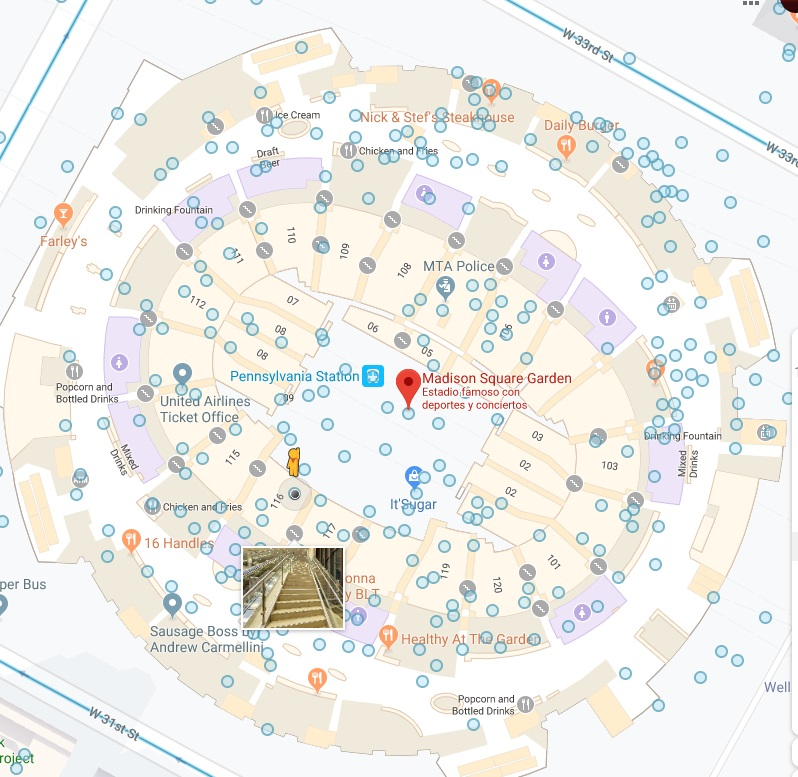
\includegraphics[width=0.6\textwidth]{Imagenes/Estadodelacuestion/MadSq2}
	\caption{Plano de un edificio proporcionado por Google Maps.}
	\label{fig:ejemplo}
\end{figure}

\begin{figure}[t]
	\centering
	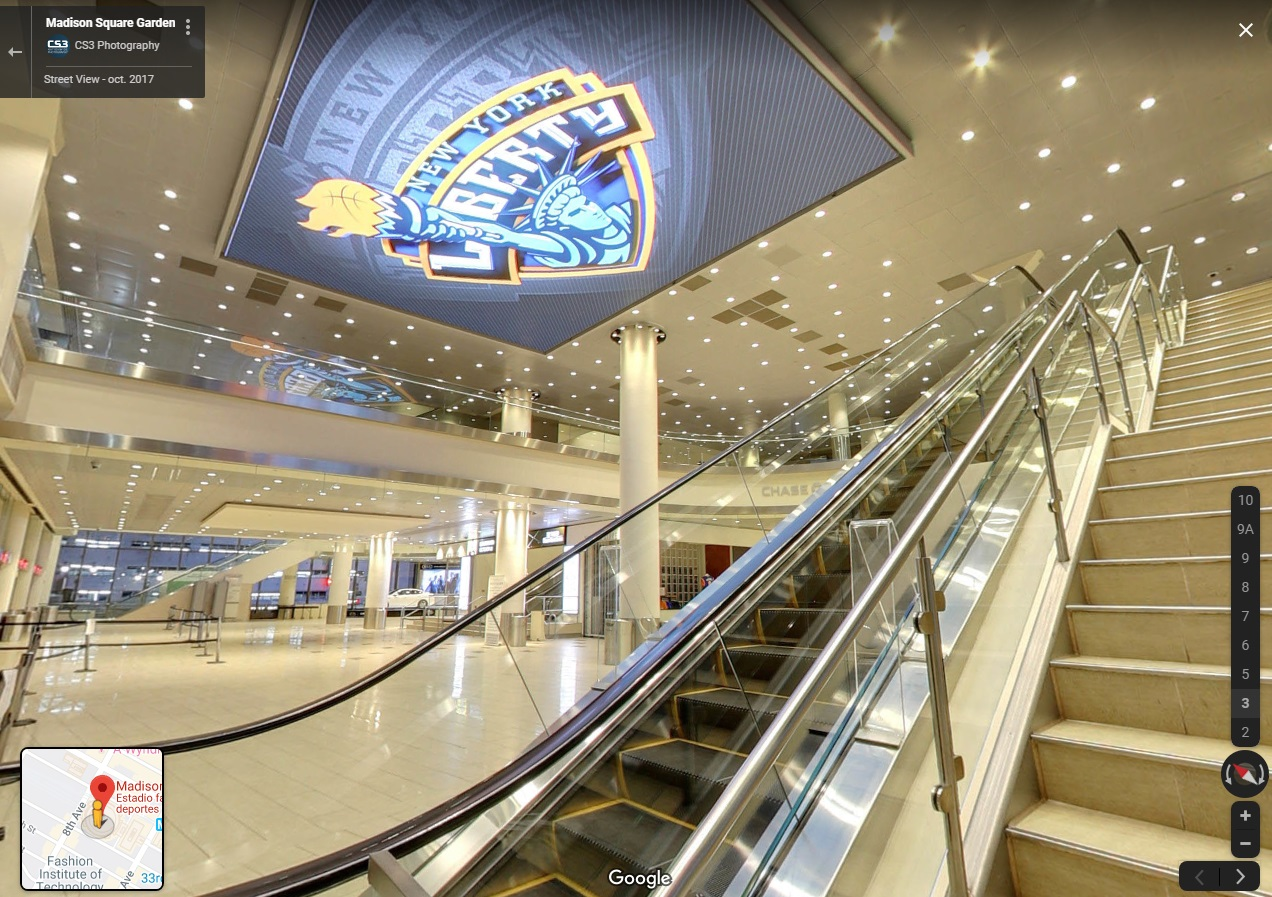
\includegraphics[width=0.6\textwidth]{Imagenes/Estadodelacuestion/MadSq3}
	\caption{Vista del interior del Madison Square Garden. }
	\label{fig:ejemplo2}
\end{figure}

En el plano podrás localizar dónde están los baños, escaleras, ascensores, entradas y salidas, etc. los cuales aparecen representados mediante los iconos globalmente aceptados (ver figura \ref{fig:ejemplo}). También aparecen detallados los distintos establecimientos que se localizan en el edificio e incluye la posibilidad de hacer ciertas búsquedas, tanto generales (de cafeterías, librerías, tiendas, restaurantes...) como concretas (Starbucks, McDonald...) (ver figura \ref{fig:ejemplo3}). Otra funcionalidad que no falta en la versión de interiores es la posibilidad de señalar un destino y recibir indicaciones sobre cómo llegar a el. Para ello, aparece el habitual punto azul que te acompaña e indica tu posición, actualizando el plano con cada movimiento que lleves a cabo (incluidos cambios de una planta a otra) (ver figura \ref{fig:ejemplo3}).

\begin{figure}[t]
	\centering
	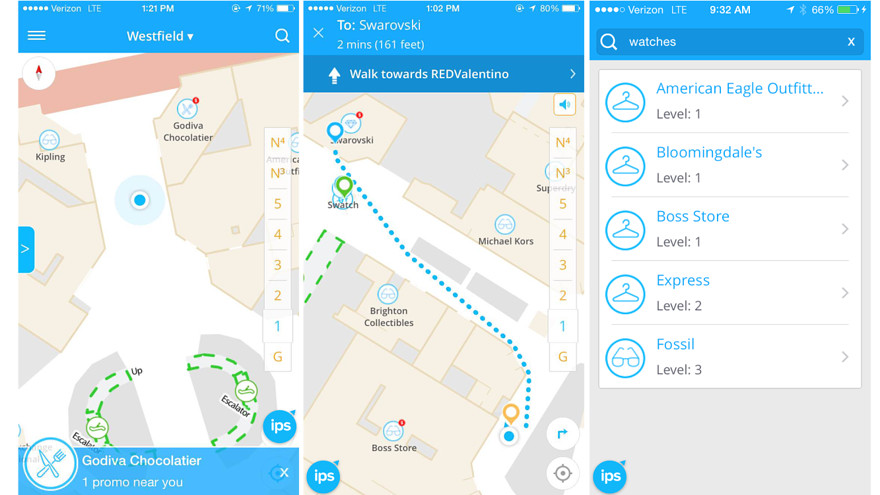
\includegraphics[width=0.6\textwidth]{Imagenes/Estadodelacuestion/GMapsInd}
	\caption{Ejemplo de navegación y búsqueda en Google Maps Indoors. }
	\label{fig:ejemplo3}
\end{figure}
Esta aplicación es un proyecto colaborativo y por ende, desde la web es posible actualizar y subir nuevos planos. Está disponible tanto para ordenador como plataformas Android e iOS.

Pese al gran avance que supone en la navegación por interiores, cuenta con ciertas desventajas. El posicionamiento, al contrario que en exteriores, no es muy preciso y las búsquedas que puedes realizar son limitadas, no pudiendo, por ejemplo, preguntar por la ubicación de los baños. Pero, sobre todo tiene el inconveniente de que no es una tecnología accesible. \textit{Google Maps Indoors}\footnote{\url{https://www.youtube.com/watch?v=cPsTWj_O3Qs}} es una aplicación completamente visual que no cuenta con soporte auditivo por lo que descarta completamente a usuarios invidentes.


%SEGUNDA APP
\subsection{BlindSquare}
Es una de las aplicaciones de navegación más populares, su uso se extiende en más de 130 países y está habilitada en 25 idiomas, entre los cuales se incluye el español. Esta aplicación, desarrollada para iOs y diseñada para personas con discapacidad visual, proporciona una guía completa, de origen a destino, tanto en exteriores como en interiores. Además, describe el entorno y anuncia posibles puntos de interés para el usuario (como pueden ser los lugares considerados populares o aquellos visitados frecuentemente). Su principal característica es que permite interactuar mediante voz gracias al controlador de música de Apple. 

\textit{BlindSquare}\footnote{\url{https://www.blindsquare.com}} determina tu posición mediante localización \textit{GPS} y, a partir de ahí, puede darte información sobre las proximidades utilizando \textit{Foursquare} y \textit{OpenStreetMap}, de este modo, es capaz tanto de guiarte a un cierto destino como de notificarte qué establecimientos hay en tu radio: restaurantes a 200m, parques más cercanos, farmacias...

Con el fin de agilizar el uso de la app y que por tanto, esta sea cómoda y rentable para los usuarios finales, incluye: accesos directos a funciones mediante gestos, como sacudir el móvil para que nos diga la ubicación actual y puntos cercanos; y, la posibilidad de establecer filtros para recibir únicamente información deseada. Filtrar por restaurantes para no tener notificaciones sobre estaciones de tren o librerías.

En cuanto a la localización por interiores, \textit{BlindSquare}\footnote{\url{https://www.youtube.com/watch?v=9jH-Bdjmgb4}} emplea \textit{beacons} y ¿¿VPS?? para solventar el problema del posicionamiento. Por lo demás, incluye las mismas posibilidades y funcionalidades que la navegación por exteriores, con la única limitación de que el edificio debe estar provisto de dichos sistemas de posicionamiento.

Entre los puntos fuertes de esta aplicación destacamos los siguientes:
\begin{itemize}
	\item Da información sobre los metros que quedan hasta llegar a un determinado objetivo. Resulta útil porque si van disminuyendo sabes que vas por el camino adecuado.
	\item Utiliza indicaciones reloj (a las 10, a las 3,...) muy usadas por las personas con discapacidad visual.
	\item Te avisa de las intersecciones. 
	\item Cuando te da una nueva indicación y la superas salta el sonido asociado a correto o check. Así, puedes seguir sin preocuparte. Si por el contrario te equivocas te salta un sonido en consecuencia.
	\item Se pueden añadir ubicaciones en una lista de lugares marcados.
	\item Puedes ir girando con el móvil y te va indicando lo que tienes enfrente. 
	\item También tiene opción de simulación, que permite prepararse un camino antes de ir.
	\item Te permite ser más autónomo y descubrir nuevos sitios.
	\item A la hora de desplazarte te indica las opciones por adelantado. Bus, metro, etc. para espacios exteriores o, escaleras, ascensor, escaleras mecánicas, etc. en el caso de interiores.
	\item Permite llevar las manos libres.
	\item Incluye un lector de códigos QR, es más cómodo porque puede dar más información que la línea braille.
\end{itemize}

Entre sus puntos negativos: su precio, cuesta 40 libras.

\subsection{Nearby Explorer}
\textit{Nearby Explorer}\footnote{\url{https://play.google.com/store/apps/details?id=org.aph.nearbyonline&hl=es}} es otra de las aplicaciones que encuadramos en el campo de la navegación accesible por interiores y exteriores. Está habilitada tanto para Android como para iOs y su descarga se encuentra disponible en el \textit{App Store} de manera gratuita. 

La guía por exteriores se basa en la misma idea que \textit{BlindSquare} y por ende, funciona de manera similar. Entre sus características destacan: la posibilidad de ejecutar ciertas acciones poniendo el móvil en distintas posiciones, como por ejemplo, inclinarlo verticalmente para que funcione como una brújula; y, la capacidad de filtrar la información de modo que ésta se adapte completamente a las necesidades del usuario. Entre la información que \textit{Nearby Explorer} puede prorporcionar a sus usuarios encontramos los lugares cercanos a la ubicación actual, los nombres de las calles por las que pasa, los números de los bloques de las calles por las que pasa, la distancia que hay al destino desde un punto de referencia (como casa, trabajo...), etc. Además de la posibilidad de filtrar la información deseada, las indicaciones por audio pueden ser pausadas en cualquier momento de modo que, no interfieran con otras señales auditivas (como las paradas en un autobús, por ejemplo). Otra gran funcionalidad con la que cuenta \textit{Nearby Explorer} es la de explorar una ruta por adelantado, sin tener que estar físicamente en el sitio, pudiendo incrementar o decrementar el radio de exploración.

Por otro lado, vemos que la navegación por interiores puede ser configurada de dos maneras: \textit{ad hoc} y \textit{mapeo completo}. Ambas utilizan los sistemas beacons para geolocalizar el dispositivo en interiores (zonas a las que no llega el \textit{GPS}) y así, poder proprocionar una guía por dicho espacio.

En el caso de la configuración \textit{ad hoc} aparecen los siguientes problemas:
\begin{itemize}
	\item No se puede determinar la ubicación de un beacon.
	\item No se puede obtener información del entorno a menos que te encuentres dentro del radio de detección de un beacon.
	\item Tienes que habilitar cierto soporte para detectar los beacons (no se detectan de manera automática).
\end{itemize}

Sin embargo, el \textit{mapeo completo} sí nos proporciona una localización precisa. Tiene un comportamiento similar al de otras aplicaciones.

\subsection{Lazarillo}
Es una aplicación que actualmente solo proporciona una guía para exteriores. Inicialmente, la idea era cubrir también la navegación por interiores pero su desarrollo no fue posible por problemas de financiación.

La navegación por exteriores cuenta con las funcionalidades básicas que ya hemos mencionado en las apps anteriores: \begin{itemize}
	\item Buscar lugares de interés, cercanos a la ubicación actual. Esta búsqueda se puede acotar filtrando por categorías que vienen predefinidas (transporte, bancos y cajeros, salud, comida, tiendas, etc.).
	\item Buscar una dirección específica a partir de la cual se desplegarán todas las posibles rutas (a pie, en transporte público, uber, etc.) y una vez seleccionada la ruta deseada, comenzarán las indicaciones mediante audio con la información pertinente (metros, giros a derecha e izquierda, etc. ). 
	\item Guardar por lugares favoritos.
	\item Posibilidad de rastrear una dirección, previamente marcada con la opcion ``Seguir este lugar'', de modo que con independencia de a dónde nos estemos dirigiendo se activará una alerta a medida que nos acerquemos a dicha ubicación.
	\item Ajustar la configuración de las indicaciones, velocidad, tipo de voz...
\end{itemize}

En resumidas cuentas, \textit{Lazarillo} es una aplicación que, como otras, busca mejorar la calidad de vida de las personas con discapacidad visual indicándoles para ello, qué les rodea y proporcionándoles una mayor independencia. Ésta, sin embargo, cubre únicamente los aspectos más básicos y elementales, sin reparar en otras posibles funcionalidades o indicaciones (véase de obstáculos, peligros...) que la convierten en una aplicación incompleta.

La app es completamente gratuita y cuenta con versión para Android y iOs.
\subsection{Wayfindr} %no he conseguido encontrar la app, por eso he puesto que no está disponible pero no estoy segura.
Es una aplicación cuyo objetivo es guiar a los invidentes por el metro de Londres (uno de los más complejos del mundo). Este proyecto, aún no disponible, pretende llegar a esos lugares que están repletos de señales escritas, por los que las personas que ven pasan sin pensar pero que son precisamente los que más temen y evitan aquellos que tienen discapacidad visual. Investigaciones llevadas a cabo en el Reino Unido revelan que la mayor parte de este colectivo querría salir de su hogar con más frecuencia. Por ello, la sociedad británica \textit{Royal Society for Blind Children (RSBC)} y \textit{UsTwoo}, plataforma de innovación y tecnología digital, se unieron para desarrollar una solución, naciendo así, Wayfindr\footnote{\url{https://www.wayfindr.net/}}.

El funcionamiento\footnote{\url{https://www.youtube.com/watch?v=mc3KmbfxuUQ}} de la aplicación es tan práctico como sencillo, se basa en una serie de sistemas Bluetooth, llamados beacons, que se colocan en las paredes de las distintas estaciones de metro emitiendo unas señales que son captadas por el móvil a su paso por un cierto radio de detección. Estas señales permiten ubicar al usuario y darle la siguiente indicación para el conseguimiento de su objetivo (coger un tren o salir de la estación).

Los desarrolladores recomiendan el uso de auriculares de conducción ósea, de manera que puedan escuchar otros sonidos del exterior.

\subsection{Conclusiones}
Tras este breve recorrido por algunas de las aplicaciones de guía adaptadas para personas ciegas o con visibilidad reducida podemos decir que cada vez son más las opciones, hemos visto desde aplicaciones de guía por exteriores, pasando por los interiores y llegando hasta algunas tan específicas como \textit{Wayfindr} para el metro de Londres. Todas ellas se rigen por un patrón común: el de la simpleza, que no va, de ninguna manera, reñida con una reducción de la funcionalidad. A pesar de simples, estas aplicaciones permiten filtrar la información que se quiere recibir, guardar lugares favoritos, su manejo mediante voz o sacudidas del teléfono, guían también mediante el uso sonidos específicos, etc.

Sin embargo, si nos centramos en guía por interiores, aún son muchas las situaciones que quedan por cubrir, ya que el \textit{mapeado} del interior de los edificios debe ser realizado de manera expresa, no es tan sencillo como ``pasear el coche de \textit{Google Maps} por los pasillos'', al menos no de momento. En la siguiente sección veremos qué tecnología podemos usar para solventar el problema del posicionamiento en interiores.


\section{Tecnología}
Nos centramos ahora en el estudio e investigación de la tecnología necesaria para realizar nuestra aplicación de guía por interiores:

\subsection{Balizas Bluetooth}

Los beacons o balizas bluetooth son pequeños dispositivos que emiten señales de radio. Estas señales los identifican de manera única y pueden ser captadas por otros dispositivos receptores, estableciendose así, un canal de comunicación que permanece vivo siempre que permanezcan en un radio de alcance entre 10 y 30 metros, como máximo. Además, estas balizas son de bajo consumo, es decir, sus baterías tienen una duración muy prolongada, aproximadamente 2 años con una simple pila de botón y su coste es reducido.

Esta tecnología se hizo muy popular en 2013, cuando Apple introdujo su iBeacon estándar y comenzó a utilizarlos para el posicionamiento por interiores. En 2015, Google, que no se quiso quedar atrás, sacó el protocolo Eddystone, un protocolo, que a diferencia del de Apple, es de código abierto y ofrece soporte oficial tanto para iOs como para Android. Los beacons provistos del protocolo Eddystone pueden ser de 4 tipos, estos tipos se distinguen por el paquete de datos que pueden emitir, véase:



\begin{itemize}
	\item \textbf{Eddystone-UID:} transmite un identificador de baliza único compuesto por 16 bytes, 10 de ellos referidos al espacio de nombres, que identifican a un grupo de beacons, y 6 que se refieren e identifican a la instancia particular dentro del grupo. Esta distinción entre espacio de nombres e instancia se pensó para optimizar el escaneo de beacons.
	\item \textbf{Eddystone-URL:} transmite una URL utilizando un formato de codificación.
	\item \textbf{Eddystone-TLM:} transmite información sobre la baliza. Esto puede incluir el nivel de la batería, los datos del sensor u otra información relevante para los administradores de balizas. Para poder usarse como baliza debe ir acompañado de otro tipo de marco (Eddystone-URL o Eddystone-UID).
	\item \textbf{Eddystone-EID:} emite un identificador encriptado que cambia periódicamente, de modo que su uso está restringido a aplicaciones y dispositivos autorizados.
\end{itemize}

Para el motivo de nuestro estudio, la navegación por interiores, esta tecnología bluetooth es muy útil, basta con colocar las balizas en puntos de interés (\textit{landmarks}) del edificio en cuestión y tener una aplicación que interprete las señales que recibe para saber donde se encuentra exactamente el usuario. No obstante, hay que tener en cuenta que la disposición exacta de los beacons y la cantidad necesaria para \textit{mapear} un área dependerá del edificio concreto.

El hecho por el cual se usa esta tecnología bluetooth y no otra, como el conocido GPS, es que las señales GPS funcionan muy mal en interiores, apenas son visibles. Además, con ellas no es posible determinar con exactitud en qué planta del edificio nos encontraríamos, por ejemplo. Para dar solución a estos problemas también se han usado las señales Wi-Fi. Esta técnica se basa en leer la señal de varios puntos de acceso Wi-Fi del edificio y, mediante triangulación, establecer el posicionamiento. Una de las ventajas del uso de la red Wi-Fi es que podemos aprovechar la infraestructura el edificio. Sin embargo, el posicionamiento basado en cliente-servidor no está soportado en dispositivos Apple (recordemos que estos fueron los primeros en sacar al mercado la tecnología beacon). Así que usando Wi-Fi estaríamos descartando de un plumazo a buena parte de los usuarios.

Entre las ventajas que nos ofrecen los beacons destaca su flexibilidad: podemos colocarlos donde queramos, son pequeños y ligeros y proporcionan una exactitud de 1 a 3 metros, frente a una de 5 a 15 con la señal Wi-Fi. 

La navegación por interiores no es el único uso que se le puede dar a los beacons. Con ellos podemos, por ejemplo, traquear de dispositivos en una oficina (como proyectores o portátiles), dar a conocer un establecimiento (la instalación de un beacon puede hacerlo más accesible, una persona ciega puede reconocer el establecimiento gracias a la señal que ha captado su móvil), el análisis de los flujos de personas en centros públicos como aeropuertos, entre otras. 




 
\chapter{Estudio de las necesidades de las personas con discapacidad visual}
\label{cap:once}

La idea de este trabajo de fin de grado surge de la necesidad de resolver problemas reales para gente real, concretamente para personas con discapacidad visual. De esta manera, empezamos nuestro camino por lo más importante: conocer las necesidades de los usuarios finales. Con este fin y gracias a la oportunidad que nos ha brindado la Universidad Complutense de Madrid con la profesora María Guijarro al frente, hemos podido reunirnos y entrevistar a personas especializadas en el campo de las tecnologías que sufren discapacidad visual.

En este Capítulo recogemos las notas que tomamos durante la reunión el pasado 11 de octubre de 2019 en el CTI (Centro de Tiflotecnología e Innovación) de la ONCE, donde nos dieron una pequeña charla sobre la ceguera y las tecnologías accesibles que han surgido para reducir la brecha, y en la que finalmente conectamos con potenciales usuarios que nos hablaron sobre sus gustos y necesidades. En la Sección \ref{sec:intro_reunion} se detalla el desarrollo de la misma, incluyendo las preguntas realizadas, las respuestas obtenidas durante la entrevista (Sección \ref{sub:entrevista}). Las conclusiones a las que se llegaron tras el posterior análisis de la misma se detallan en la Sección \ref{sec:conclu_ONCE}. 


\section{Reunión en el Centro de Tiflotecnología e Innovación de la ONCE}
\label{sec:intro_reunion}
La visita al CTI comenzó con una breve explicación, de la mano de José María Ortiz, director del Departamento de Consultoría e Innovación, sobre las principales tareas que se llevan a cabo en el centro, entre las cuales destacan:

\begin{itemize}
	\item Ayudar a una persona con discapacidad visual en su \textbf{adaptación} al trabajo y a la vida cotidiana, proporcionandole para ello el material necesario (teclados, líneas de braille, bastones, etc.).
	\item Responder a \textbf{consultas} sobre el funcionamiento de dispositivos.
\end{itemize}

Luego, nos comentó los departamentos en los que se estructura el centro para que pudiésemos hacernos una idea más global de todo lo que abarca. Éstos son:

\begin{itemize}
	\item \textbf{El departamento de Consultoría e Innovación}, donde actualmente están desarrollando el programa EDICO\footnote{\url{http://cidat.once.es/home.cfm?id=2351&nivel=2}} en colaboración con la UCM, que tiene como objetivo hacer las matemáticas accesibles mediante un editor de texto. De manera paralela se encargan del desarrollo de aplicaciones de muy diversa índole, véase apps para la biblioteca de la ONCE, de películas audio-descritas, etc.
	\item \textbf{Departamento de Evaluaciones y Auditoría}, donde se encargan de evaluar los productos que se van a sacar al mercado.
	\item \textbf{Departamento de Diseño y Producción}, donde se encargan de, tal y como indica su nombre, diseñar y producir elementos de adaptabilidad, como pueden ser unas plantillas con relieve de policarbonato para las vitrocerámicas. Recordemos que estas, aunque no presentan dificultad alguna para los usuarios videntes, son tediosas para aquellos que cuentan con discapacidad visual ya que la pantalla táctil no tienen ningún tipo de relieve que pueda servirles como referencia y guiarles en su uso.
	\item \textbf{Departamento de Asesoría en Tecnología}, especializado en tecnologías accesibles.
\end{itemize}

Una vez concluida esta sección en la que nos contextualizaron, abrieron paso a la ronda de preguntas en la que pudimos acercarnos a ellos, conociendo sus problemas y necesidades en el día a día.


\subsection{Entrevista}
\label{sub:entrevista}

Durante esta parte, nos dirigimos especialmente a Mónica y José Luis Llorente, ambos ingenieros del CTI, para que, con su experiencia y conocimientos, nos explicaran lo máximo posible sobre tecnologías accesibles y nos dieran su punto de vista en las ideas que proponíamos. Por otro lado, Mónica no solo era experta en la materia sino que además es invidente, por lo que nos pudo contar su perspectiva y necesidades como usuaria.

Las preguntas avanzaron desde temas generales para conocer cómo una persona invidente se desenvuelve con la tecnología, sus gustos y qué sensaciones le despierta, hasta temas concretos dirigidos a conocer los problemas que plantea la navegación por espacios interiores:

\begin{itemize}
	\item  \textbf{¿Cómo utiliza una persona con discapacidad visual un dispositivo móvil?}
	
	Para responder a esta pregunta, Mónica nos hace una demostración en directo. Para ello emplea un móvil Xiaomi con sistema operativo Android.
	
	Mónica nos cuenta que para la navegación por su dispositivo utiliza un lector de pantalla, es decir, un software que facilita el uso del sistema operativo. Éste sirve como guía para las personas que, como ella, tienen discapacidad visual, ya que ``lee y explica'' mediante voz lo que se ve en la pantalla. Los lectores de pantalla vienen siempre incluidos en el dispositivo y se pueden encontrar en la sección de Accesibilidad, en Ajustes. En el caso de Android, este software se llama \textit{Talkback} y es configurable. Por ejemplo, dice Mónica, se podría usar mediante la línea de braille en vez de la reproducción por voz.
	
	Luego vemos como se desplaza por las aplicaciones utilizando \textit{flicks}, movimientos secos en los que desliza el dedo hacia uno de los lados de la pantalla (izquierda o derecha, según interese). Del mismo modo, para la navegación por la web o dentro de alguna aplicación utiliza estos movimientos hacia arriba y hacia abajo. Por último, nos muestra cómo accede a un elemento mediante doble click. 
	
	También nos habla de la posibilidad de la navegación libre, eso sí, solo cuando ya te has familiarizado con el dispositivo lo suficiente como para saber dónde tienes determinadas aplicaciones. 
	
	Lo más cansado, según Mónica, es tener que hacer un barrido por toda la pantalla hasta encontrar lo que quieres, en vez de poder ir directamente. Para agilizar un poco este proceso, Mónica, por ejemplo, agrupa las aplicaciones por carpetas, de modo que el barrido es más sencillo que si la pantalla estuviese repleta.
	
	Para las personas con baja visión también existe la posibilidad de hacer más grandes los iconos y ajustar los colores.
	
	% Segunda pregunta:
	\item \textbf{Hemos leído que normalmente las aplicaciones se desarrollan para dispositivos iOS, ¿por qué es mejor?} 
	
	\textit{``Si que es cierto que solía ser así ya que iOS le llevaba la delantera a Android en cuanto a accesibilidad, pero cada vez se usa más Android pues las diferencias están completamente recortadas, están muy igualados y los precios son mucho más asequibles. Yo misma antes tenía un iPhone y ahora me he pasado a Android y no hay nada que eche en falta.''}, responde Mónica.
	
	% Tercera pregunta:
	\item \textbf{¿Cómo afronta una persona ciega su desplazamiento y orientación por interiores cuando pisa por primera vez dicho espacio u edificio?}
	
	Ante esta pregunta Mónica resopla y nos contesta: \textit{``Buufff..., ¿te vale?''}
	
	Nos puso como ejemplo la llegada a un hospital: \textit{``cuando entras necesitas saber, al menos, dónde está la recepción para pedir ayuda pero los carteles informativos están fuera de mi alcance, entonces entro por la puerta y pienso ¿y ahora qué?. ¿Dónde está el mostrador de recepción? No es tan fácil como echar un primer vistazo, necesitas ayuda mediante voz, algo que te describa el espacio y te vaya diciendo que hay a derecha e izquierda y a cuantos metros.''}
	
	Nos contó que en cuanto a la descripción/guía por espacios interiores ahora mismo no hay disponible ninguna aplicación. Por ello, una vez superada la primera barrera de ubicar y localizar un cierto destino, la única opción que les queda es la de memorizar el camino. Mónica destacó que era increíble la cantidad de rutas que tiene en la cabeza.
	
	Por todo esto, se comentó que una aplicación del tipo que se quiere implementar en este trabajo de fin de grado sería de gran ayuda para ellos. No solo para que les guiase hasta un punto concreto, sino para que también describiese el edificio, facilitándoles una primera idea del mismo que les ayudase a moverse con mas seguridad y les indicase qué posibilidades les ofrece. En este punto se mencionaron otras propuestas e ideas sobre cómo proporcionar esta información estática del edificio. Algunas de ellas fueron: 
	
	\begin{itemize}
		\item[$-$] Tener subido el plano de las distintas plantas del edificio e implementar un sistema de manera que cuando se deslice el dedo sobre las distintas salas que aparecen la app indique cuales son (aula X, cafetería, secretaría, pasillo, etc.).
		\item[$-$] La impresión de un mapa 3D que disponga de un código QR o algo similar que sea capturado por Bluetooth (mejor que por foto) y que tras leerlo cargue el plano del edificio y pueda proporcionar tanto información sobre el espacio en sí mismo (número de plantas, qué hay en cada una...) como información cambiante como la existencia de averías, horarios, disponibilidad de salas, etc.
	\end{itemize}
	
	Como es natural, de la mano de estas ideas surgieron problemas y opiniones a favor y en contra: ¿Dónde estaría dicho mapa?, ¿Cómo encontrarlo?, ¿Todos los edificios estarán de acuerdo en facilitar los planos o puede que por motivos de seguridad no sea una idea factible?, ¿Es posible llegar a un standard para que se pueda usar el mismo sistema en cualquier edificio?
	
	% Cuarta pregunta:
	\item \textbf{¿Hay algún tipo de señales que os sirvan como referencia a la hora de desplazaros por un edificio?}
	
	\textit{``Hay señales de encaminamiento, que te indican dónde están las escaleras, ascensores, zonas de cruce, etc.''}, contesta.
	
	% Quinta pregunta:
	\item \textbf{¿Cuántos edificios cuentan con estas señales?}
	
	\textit{``La verdad que cada vez son más frecuentes y hoy en día se encuentran en casi todos los edificios, especialmente en los nuevos.''}, responde.
	
	% Sexta pregunta:
	\item \textbf{¿Cómo de factible es ir con el dispositivo móvil en la mano, para realizar una foto o cualquier cosa similar?}
	
	\textit{``Puedo hacer una foto en un momento puntual, en eso no hay problema alguno pero no es cómodo ir con el móvil en la mano constantemente porque además de que es aparatoso porque ya llevo en la mano el bastón, perro guía, etc. No es práctico, no sería la primera vez que roban un móvil a una persona invidente, es una realidad.''}, contesta Mónica. \textit{``Particularmente, con respecto a la foto el problema principal sería saber a dónde enforcar''}, añade.
	
\end{itemize}

%Creo que es mejor subsection para las conclusiones del TIC
%TERCERA SECCIÓN
\section{Conclusiones}
\label{sec:conclu_ONCE}

Una vez finalizado el debate y, tras poner en común las notas recogidas durante la entrevista, se establecieron una serie de puntos clave sobre los que guiar nuestro proyecto. Estos ponen de manifiesto la necesidad de una aplicación como la nuestra y nos dan información sobre qué funcionalidades deben estar presentes y cuáles no, atendiendo a sus necesidades. El resumen de esos puntos se expone a continuación:

\begin{itemize}
	\item La implementación de una aplicación como la nuestra es muy útil y necesaria.
	\item Las modalidades más empleadas para interactuar con el móvil cuando tienes algún tipo de deficiencia visual son: flicks, sacudidas, mediante vibración, arrastrando o pulsando la pantalla con un dedo, dos, etc.
	\item No resulta cómodo ir barriendo el espacio con la cámara del móvil.
	\item El uso de dispositivos adicionales como una micro cámara, en principio, no sería un problema, siempre y cuando no la tengan que llevar de manera continuada en la mano.
	\item En caso de auriculares, se recomienda utilizar auriculares óseos de modo que dejen el canal auditivo libre para captar otros estímulos.
	\item El objetivo es que el grueso de las aplicaciones sean lo más inclusivas posibles, es decir, que su uso sea apto tanto para personas videntes como invidentes.
	\item El feedback de la aplicación no debe saturar pero sí se aconseja que sea constante para que no se malinterprete que la aplicación ha dejado de funcionar.
\end{itemize}

\chapter{Mapeo de interiores mediante balizas bluetooth}
\label{cap:descripcionTrabajo}

En este capítulo explicamos el estudio realizado sobre el funcionamiento de los \textit{beacons} y su efectividad en el posicionamiento de interiores, concretamente en la Facultad de Informática de la UCM. Este trabajo de investigación ha sido muy satisfactorio ya que nos ha facilitado la toma de numerosas decisiones con las que elaborar una propuesta en resolución al mapeo del edificio y a la disposición concreta de las balizas que optimice el posicionamiento. 
%También ha contribuido a resolver algunos aspectos de la implementación que narraremos en el capítulo \ref{cap:diseñoeimplementación}.

\section{Estudio de la precisión del posicionamiento mediante los \textit{beacons}}

Una vez que hemos concluido, por las razones expuestas en la Sección \ref{sec:conclusionesposicionamiento}, escoger los \textit{beacons} como sistema de posicionamiento, vamos a realizar un estudio profundizando en los aspectos tecnológicos de estas balizas. El objetivo es comprender por completo su funcionamiento y comportamiento a la hora de medir distancias, es decir, cuánto rango tiene la señal bluetooth, con ayuda de qué función podemos recibir esta señal e interpretarla para determinar la distancia, qué margen de error presenta, en qué lugares es más aconsejable establecer las balizas para recibir mejor la señal y, por tanto, reducir el error, cómo de precisa es la distancia medida cuando el dispositivo móvil que recibe la señal bluetooth está en movimiento, etc. 

Los \textit{beacons} utilizados para este proyecto cuentan con una SDK (Kit de Desarrollo Software) propia de su marca (\textit{Kontakt}) en la que incluyen funciones ya implementadas que nos permiten conocer qué \textit{beacons} están en nuestro rango en un momento determinado y a cuántos metros están. Esta información se va actualizando cada cierto tiempo. También incluye un sistema de categorías en función de cómo de cerca o lejos esté un cierto dispositivo. Las categorías son las siguientes:

\begin{itemize}
	\item \textit{IMMEDIATE:} Si el dispositivo se encuentra a menos de $0,5$ metros.
	\item \textit{NEAR:} Si el dispositivo se encuentra entre $0,5$ y $3$ metros.
	\item \textit{FAR:} Si el dispositivo se encuentra a más de $3$ metros.
	\item \textit{UNKNOWN:} Si se ha perdido la señal del dispositivo.
\end{itemize}

Una vez descubiertas estas funciones y comprendido el código decidimos desarrollar dos pequeñas aplicaciones que sirviesen para un doble propósito. Por un lado, para tener una primera toma de contacto con el entorno de programación escogido, Android Studio, y con la incorporación de las funciones ofrecidas por la librería de \textit{Kontakt}. Y por otro, para analizar la precisión de la señal bluetooth (con y sin movimiento), concretar la posición óptima de los \textit{beacons} y desarrollar una primera idea sobre la estructuración de la información relevante del edificio en el mapeo y la implementación del código relativo al posicionamiento en el edificio. En las siguientes secciones presentamos las dos aplicaciones desarrolladas para estos fines.


\subsection{Aplicación \textit{miniapp}}
Esta aplicación constituye la primera toma de contacto con los \textit{beacons} y con el código de la SDK. Presenta una interfaz sencilla en la que aparece una tabla con las distintas categorías de proximidad para 3 balizas y, debajo, el espacio donde se indica el identificador de la baliza correspondiente. En el cuadro inferior aparecen dos botones muy intuitivos con los que el usuario puede interactuar con la app: Stop Scanning y Start Scanning. De esta manera, una vez que empieza el escaneo y las balizas se encuentran en el radio de detección, se incluyen los identificadores en cuestión y se colorea en verde la categoría de proximidad estimada en cada caso según corresponda. La lectura de los \textit{beacons} se actualiza cada 2 segundos, tiempo establecido de antemano. En la Figura \ref{fig:miniapp} podemos ver la interfaz descrita.

La idea que subyace al desarrollo de esta aplicación es introducirnos en Android Studio y manejar las funciones ofrecidas por la SDK de \textit{Kontakt}, de ahí que hayamos creado una primera interfaz con botones, cambios de color, cuadros de texto, etc. Una vez hecho esto, comprobamos que las funciones preestablecidas por la SDK funcionaban y realizamos distintas pruebas en una posición fija para establecer el grado de confianza que podíamos tener en las categorías de proximidad definidas por \textit{Kontakt}. El resultado fue muy positivo puesto que, en su mayoría, la categoría asignada se ajustaba a la realidad. Sin embargo, nos faltaba saber la precisión estricta de los \textit{beacons} al recibir la distancia exacta en metros. Por ello creamos una segunda aplicación que, aunque fuese menos visual desde el punto de vista de la interfaz, nos diese más información sobre los \textit{beacons} detectados.

\subsection{Aplicación \textit{cuadrantes\_v1}}
 \textit{Cuadrantes\_v1} es una aplicación austera. En ella aparece un gran cuadro de texto que ocupa practicamente la totalidad de la pantalla y dos botones que se sitúan en el cuadro inferior,  Stop Scanning y Start Scanning, a través de los cuales el usuario puede interactuar con la app. Su funcionamiento es sencillo e intuitivo: cuando el usuario pulsa Start Scanning comienza el escaneo de balizas y cuando una o varias entran en el radio de detección, la app plasma su información (identificador, distancia en metros y categoría de proximidad) en el cuadro de texto. Esta información se actualiza cada 2 segundos (tiempo configurable) hasta que el botón Stop Scanning es pulsado, momento en el cual cesa el escaneo. La Figura \ref{fig:cuadrantesv1} muestra la interfaz de la aplicación descrita.

Como mencionamos anteriormente, hemos creado esta aplicación con el fin de obtener más información sobre el error cometido a la hora de determinar la distancia en metros a la que se encuentran los \textit{beacons} (tanto si el dispositivo se encuentra parado como en movimiento), así como para estudiar cuales son los factores que alteran su señal. De esta manera podremos determinar los puntos claves donde colocar las balizas y abordar, tras ello, el mapeo del edificio. De ahí que el nombre de la aplicación sea \textit{cuadrantes\_v1} ya que, como veremos, los cuadrantes serán una pieza fundamental en el mapeo. A continuación exponemos las pruebas realizadas con ayuda de esta aplicación y algunas de las consecuencias derivadas de los resultados.

\begin{figure}
	\centering
	\subfloat[Interfaz de miniapp]{
	\label{fig:miniapp}
	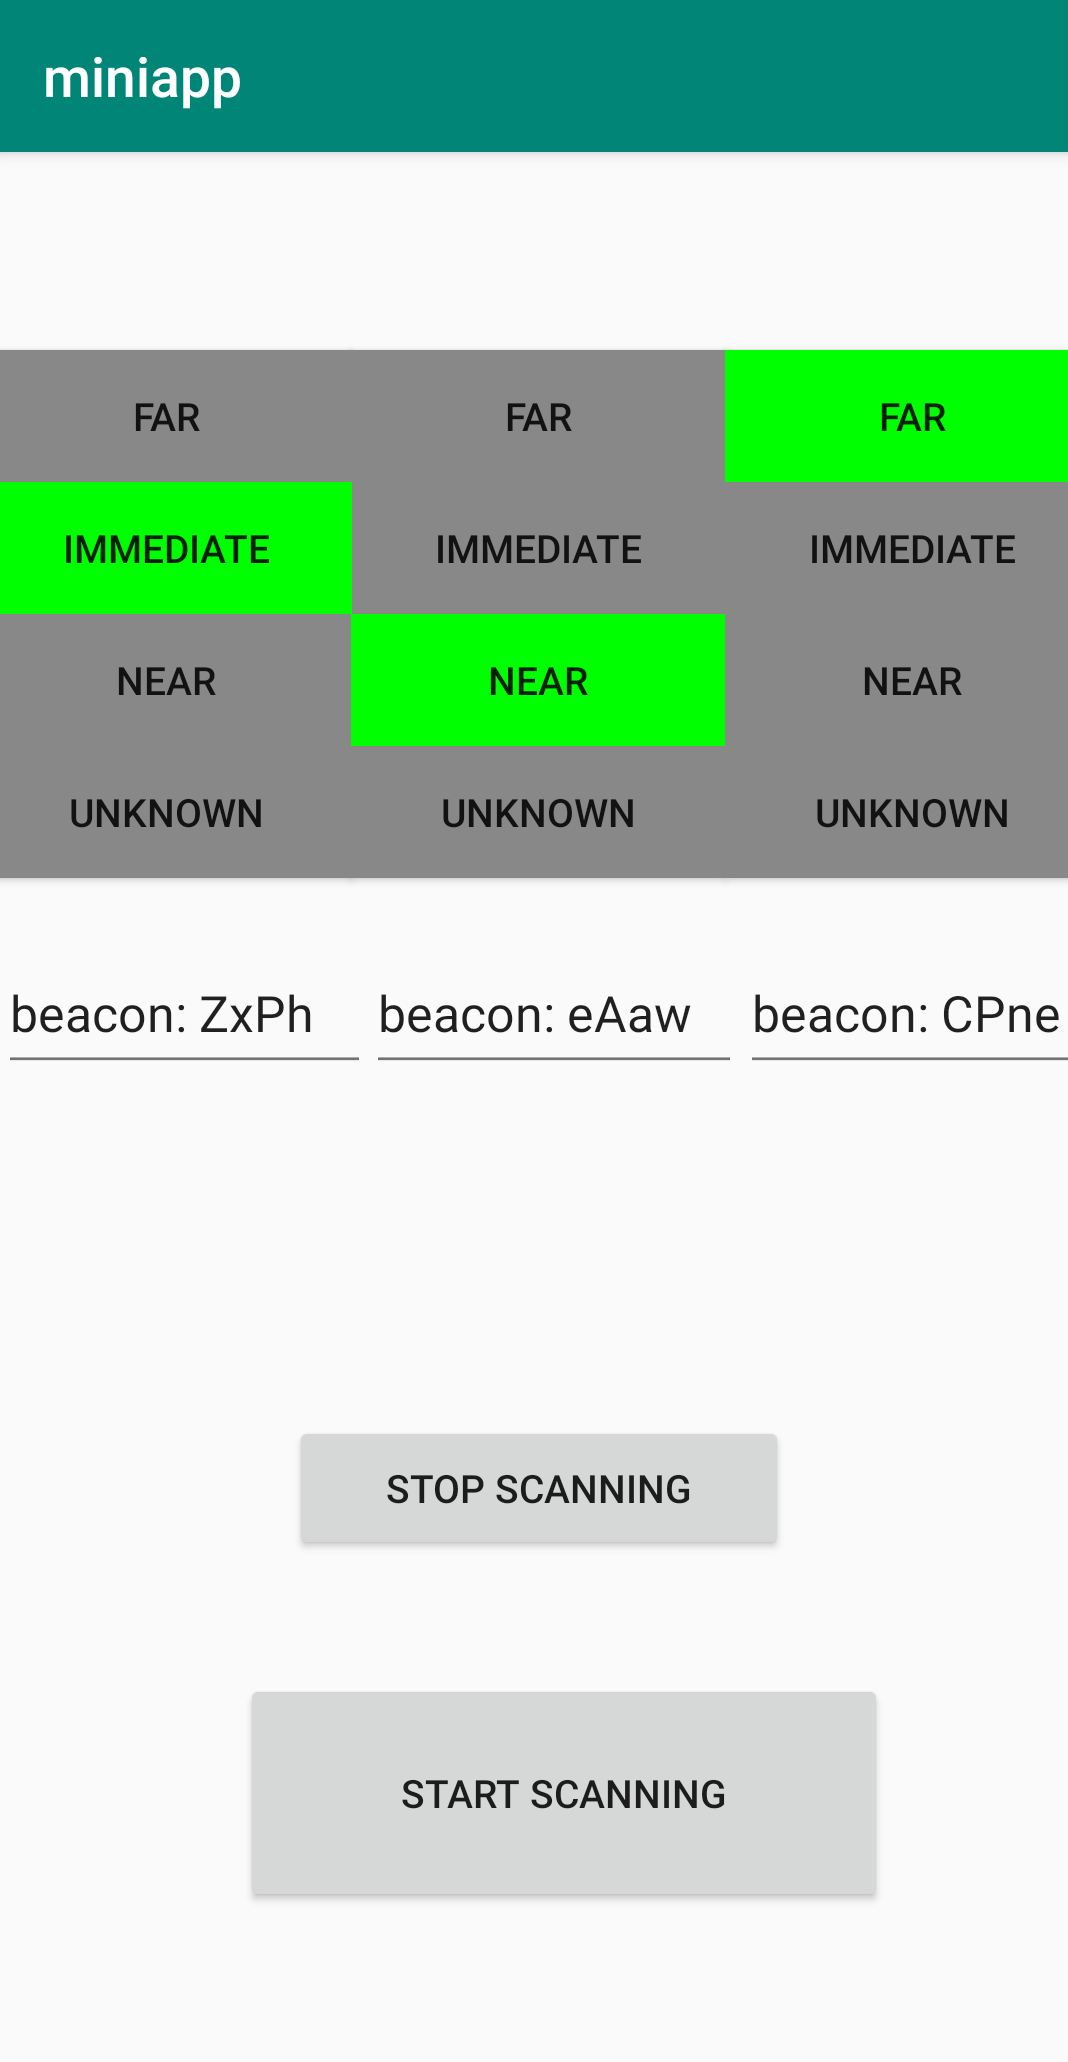
\includegraphics[width=0.3\textwidth]{Imagenes/Descripciondeltrabajo/miniapp}}
	\subfloat[Interfaz de cuadrantes\_v1]{
	\label{fig:cuadrantesv1}
	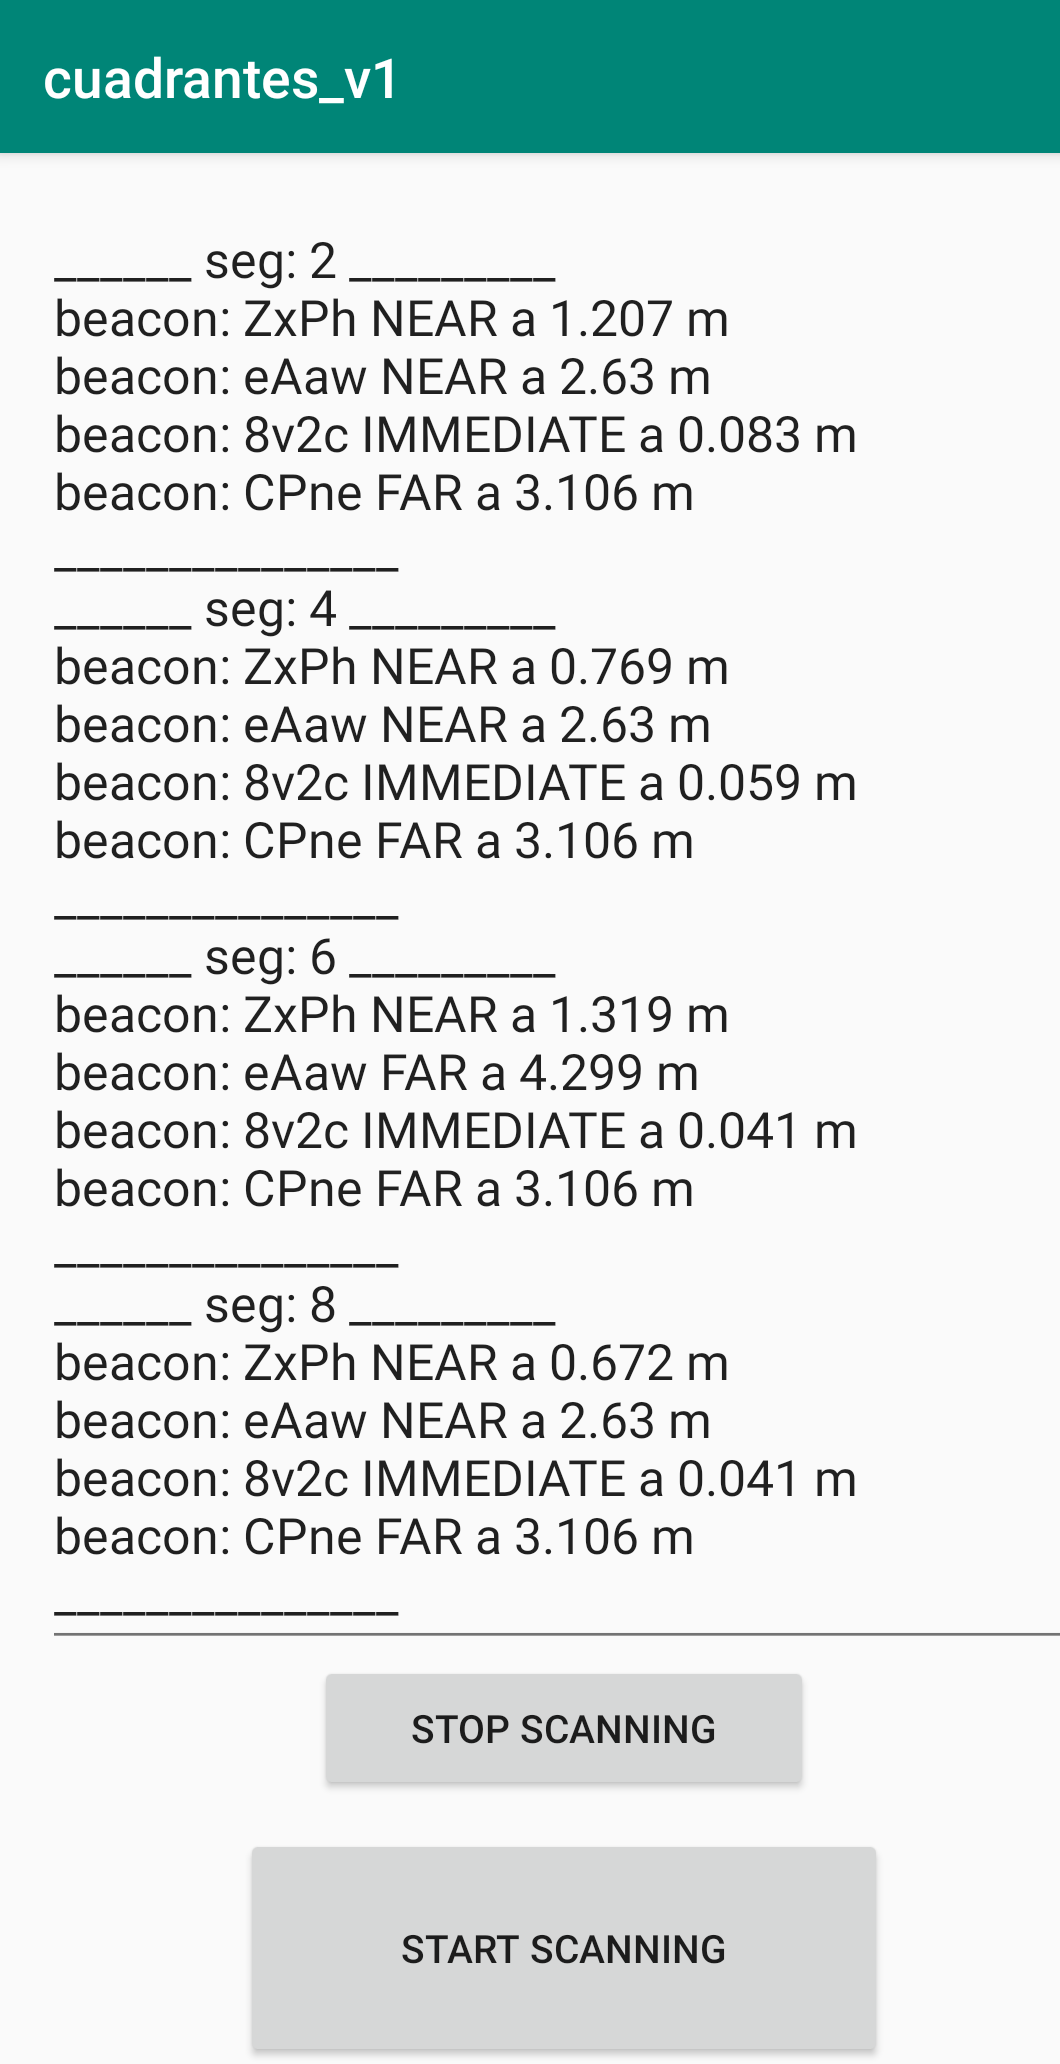
\includegraphics[width=0.3\textwidth]{Imagenes/Descripciondeltrabajo/cuadrantes_v1}}
	\caption{Aplicaciones auxiliares}
	\label{f:apps}
\end{figure}

\subsubsection{Pruebas con \textit{cuadrantes\_v1}}

Las primeras pruebas realizadas con la aplicación \textit{cuadrantes\_v1} han consistido en colocar tres \textit{beacons}, concretamente aquellos con identificadores CPne, 8v2c y eAaw, en distintos puntos de la Facultad de Informática y observar la distancia registrada desde un dispositivo móvil ubicado en un punto fijo. De esta manera, hemos podido medir el error cometido en cada caso y estimar las posibles interferencias. Para mostrar los resultados hemos creado tres gráficas que muestran la distancia a la que se detectan las balizas a lo largo del tiempo y la medida real a la que estaban situadas. 

En la Figura \ref{fig:dist_CPne} vemos las lecturas que nos ha proporcionado la aplicación \textit{cuadrantes v1} del \textit{beacon} con identificador CPne. En este caso, hemos realizado 4 estudios independientes marcados con distintos colores: azul -\textit{beacon} a 64cm, naranja -\textit{beacon} a 2m, gris -\textit{beacon} a 2,5m y amarillo -\textit{beacon} a 5 metros-. De esta gráfica concluimos que cuanto mayor es la distancia a la que se encuentra la baliza, véase la función amarilla (5m), más fluctúa la medida estimada convirtiéndose en un dato poco fiable. Correlativamente, a menor distancia menor error. Podemos ver que la función naranja (2m) es bastante fiel a la realidad, fluctúa en un intervalo de un metro a lo largo de toda la medición. Por último, el resultado de la gráfica azul (64cm) es bastante preciso, presenta un error despreciable durante toda la medición.

\begin{figure}[t]
	\centering
	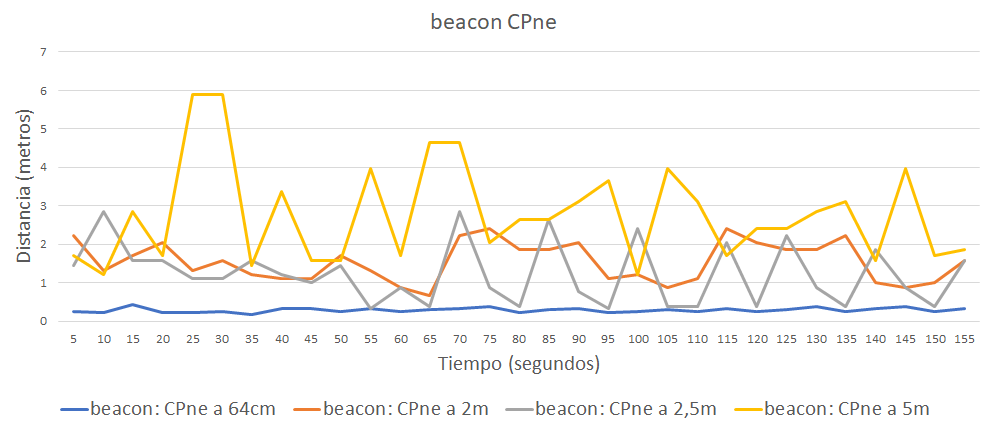
\includegraphics[width=0.8\textwidth]{Imagenes/Descripciondeltrabajo/dist_CPne}
	\caption{Gráfico con las distancias medidas al beacon CPne. }
	\label{fig:dist_CPne}
\end{figure}

En el caso de la Figura \ref{fig:dist_eAaw}, en la que se estima la distancia para el \textit{beacon} eAaw, pero usando distancias más pequeñas, el comportamiento es similar. En líneas generales, el valor medio estimado se corresponde con la distancia real a la que se encuentran las balizas. Sin embargo, en esta medición hemos contemplado una novedad que se ha repetido en numerosas ocasiones convirtiéndose en un patrón de comportamiento y es que durante los primeros segundos en los que arranca la aplicación, las estimaciones son menos precisas, dando lugar a picos importantes que más tarde se suavizan. 
\begin{figure}[t]
	\centering
	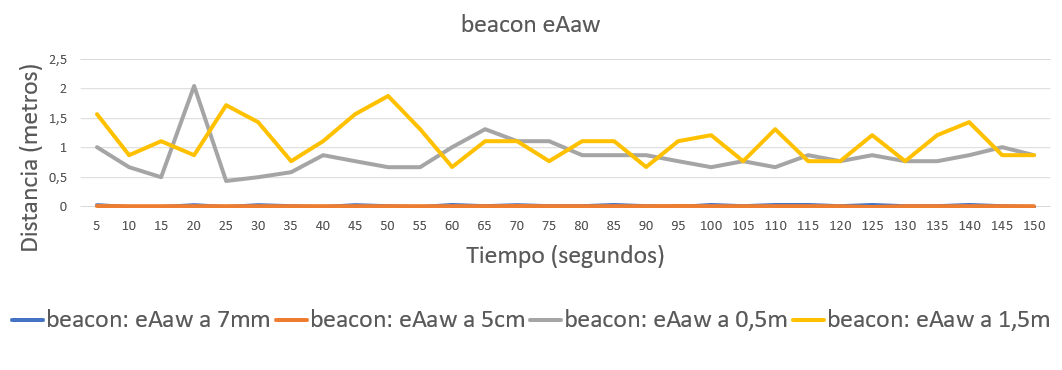
\includegraphics[width=0.8\textwidth]{Imagenes/Descripciondeltrabajo/dist_eAaw}
	\caption{Gráfico con las distancias medidas al beacon eAaw. }
	\label{fig:dist_eAaw}
\end{figure}

La Figura \ref{fig:dist_8v2c} recoge cuatro mediciones para el \textit{beacon} 8v2c, tres de ellas tomadas para una misma distancia (4m) y una a 64 cm. Observamos de nuevo que el error es despreciable cuando la baliza se encuentra muy próxima. Por el contrario, los valores que recogen las gráficas en las que el dispositivo se encuentra a 4m están muy por debajo de lo esperado, y solo una de ellas alcanza el valor real y en todas las direcciones. Este factor común nos reveló una alteración considerable de la intensidad de la señal por lo que empezamos a entrever que había factores en el entorno que la debilitan. Es por esto que la última gráfica, plasmada en la Figura \ref{fig:dist_conjunto}, hace referencia a una situación particular. Se trata de dos \textit{beacons} diferentes situados a la misma distancia uno encima del otro. El objetivo de este estudio era ver si uno de los factores que podía alterar la intensidad de señal era la presencia de otras balizas, y efectivamente como podemos observar, la intensidad de ambas señales es bastante más baja de lo esperado, prácticamente en ningún momento alcanzan el valor real. En este caso particular, el error es tolerable ya que los \textit{beacons} están situados a muy poca distancia pero sí nos advierte de que la señal bluetooth es sensible a interferencias provocadas por otros \textit{beacons} del entorno, lo cual hemos de tener muy presente a la hora de determinar la ubicación de los beacons a lo largo de la facultad para no colocarlos demasiado próximos. En la Sección \ref{sec:Interferencias} del Capítulo \ref{cap:estadoDeLaCuestion} se han expuesto algunas de las causas de las interferencias.
\begin{figure}[t]
	\centering
	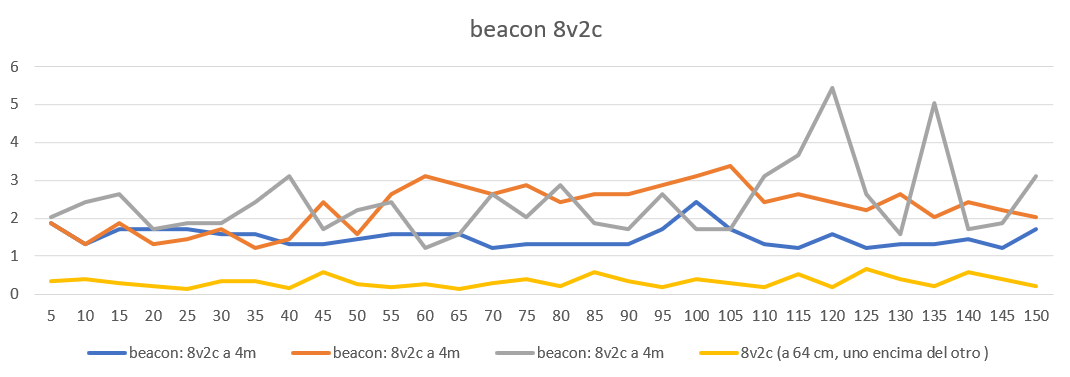
\includegraphics[width=0.8\textwidth]{Imagenes/Descripciondeltrabajo/dist_8v2c}
	\caption{Gráfico con las distancias medidas al beacon 8v2c. }
	\label{fig:dist_8v2c}
\end{figure}
\begin{figure}[t]
	\centering
	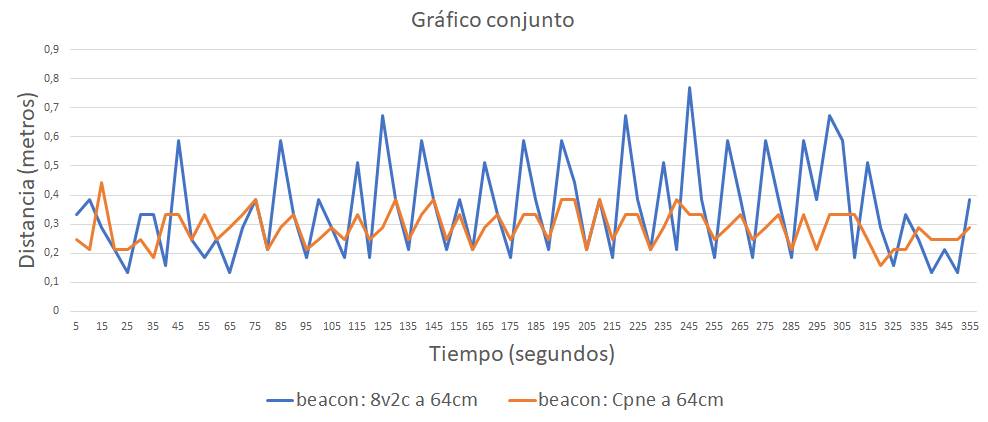
\includegraphics[width=0.8\textwidth]{Imagenes/Descripciondeltrabajo/dist_conjunto}
	\caption{Gráfico de los beacons 8v2c y CPne superpuestos. }
	\label{fig:dist_conjunto}
\end{figure}

\subsection{Conclusiones de la precisión de los \textit{beacons}}
\label{sub:conclusiones_posicionam}
Con todos estos resultados hemos decidido que para el posicionamiento utilizaremos el dato del \textit{beacon} más cercano ya que es la medida más fiable (por estar a menos metros del dispositivo) y consideraremos que el usuario se encuentra en las inmediaciones de dicho \textit{beacon}. En la Sección \ref{sec:mapeo} especificaremos la asociación realizada entre ``las inmediaciones de un \textit{beacon}'' y un punto concreto de la Facultad de Informática.

Con esta idea hemos desarrollado una primera aplicación de prueba que además de captar el \textit{beacon} más próximo al usuario emite un pitido a mayor o menor frecuencia según su categoría de proximidad. Esta app se llama \textit{pruebaSonido} y presenta la misma estética que \textit{cuadrantes\_v1}. Su funcionamiento es sencillo: al iniciar el escaneo capta el \textit{beacon} más cercano y lo fija. Tras ello, actualiza su información (concretamente, la distancia registrada y la categoría de proximidad) y pita a una frecuencia u otra según la distancia a la que se encuentre el \textit{beacon} (cuanto más cerca, el pitido es más rápido y se ralentiza a medida que la baliza está a mayor distancia). La actividad continúa hasta que el botón Stop Scanning es pulsado. Al igual que en \textit{cuadrantes v1} la información sobre las balizas detectadas queda plasmada en el cuadro de texto.

El objetivo de \textit{pruebaSonido} no es solo generar un primer código que seleccione el \textit{beacon} más cercano sino también llevar a cabo las primeras pruebas de estimación de la distancia a la que se encuentran las balizas en movimiento. Estos resultados han sido muy similares a los obtenidos estáticamente: la estimación sigue siendo más precisa cuanto más próxima está la baliza del dispositivo que la rastrea. Sin embargo, hay que ajustar el tiempo de actualización del escaneo si se quiere caminar a mayor velocidad (para que la aplicación reaccione en tiempo real y no sufra retrasos). Tras diversas pruebas hemos concluido que 2s es una medida óptima en lo que a nuestra aplicación concierne ya que nuestros usuarios, al presentar discapacidad visual, no caminan especialmente rápido. Por otro lado, esta aplicación nos ha servido también para incluir sonidos. Esto puede parecer insignificante, pero si nos paramos a pensarlo hay muchísimos sonidos que tenemos asociados con determinadas acciones, situaciones y/o aplicaciones que sin darnos cuenta nos guían en su uso y nos proporcionan la seguridad de que estamos utilizándola bien o la certeza de que tenemos que rectificar. Este recurso es indispensable en nuestra app ya que nuestros principales usuarios no podrán ver la aplicación.


\begin{figure}[t]
	\centering
	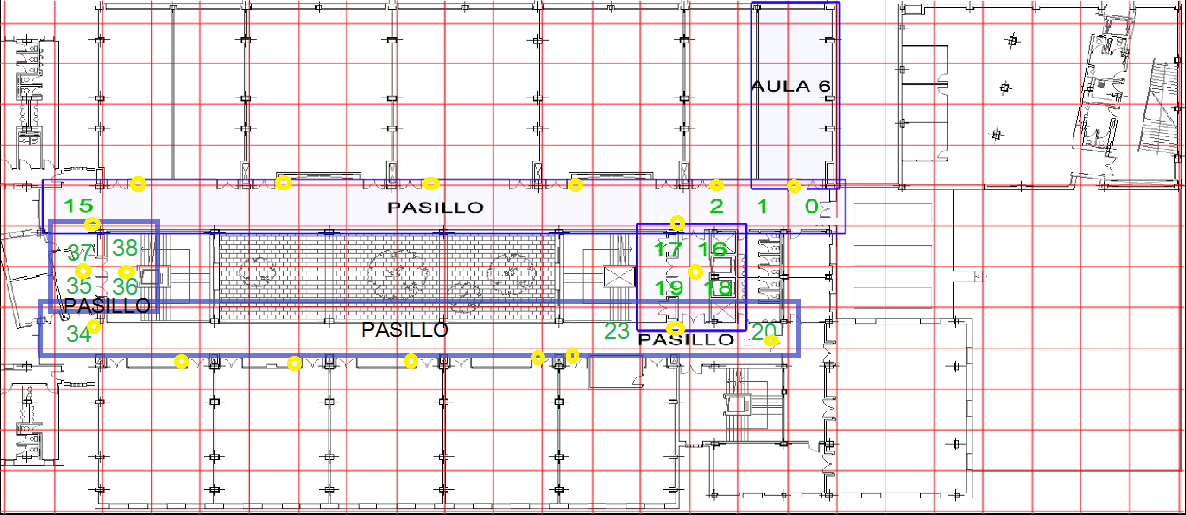
\includegraphics[width=1\textwidth]{Imagenes/Descripciondeltrabajo/mapaplanta1_cuadrantes}
	\caption{Primera versión del mapeo de la primera planta de la Facultad de Informática.}
	\label{fig:cuadrantesP1_v1}
\end{figure}



\section{Mapeo del edificio de la Facultad de Informática}
\label{sec:mapeo}

Para el mapeo de la Facultad de Informática nos hemos apoyado fundamentalmente en el proyecto de TFG \textit{Generador interactivo de instrucciones de guía sobre plataformas móviles} \citep{TFGguia}. De este, hemos reutilizado el sistema de estructuración basado en plantas que a su vez se dividen en cuadrantes con identificador único, lo que facilita determinar la planta en la que nos encontramos.
Originariamente, cada cuadrante se correspondía con nueve baldosas aproximadamente, tanto en el largo como en el ancho, y los cuadrantes se juntaban formando estancias (pasillos, aulas, etc.). De esta manera quedaban definidas cada una de las plantas del edificio y así empezamos definiendo también las nuestras. Sin embargo, sus cuadrantes contaban con dos números asociados que hacían referencia a las coordenadas sureste y noroeste que empleaban en el posicionamiento mediante triangulación Wi-Fi. Este es el primer cambio que hemos implementado ya que carecen de sentido en un posicionamiento como el nuestro, que se basa en puntos de decisión. En su lugar, debemos asociar los \textit{beacons} a los cuadrantes correspondientes. Para ello, empezamos determinando que no todos los cuadrantes tendrían una baliza asociada, sino que serían solo aquellos que tuviesen un punto de decisión. En la Figura \ref{fig:cuadrantesP1_v1} mostramos el primer acercamiento al mapeo de la planta 1 con los cuadrantes originales (en rojo), su identificador (en verde), algunas estancias (en azul) y la posición final de los \textit{beacons} (en amarillo). La disposición de los \textit{beacons} y su evolución hasta alcanzar la posición final se explicará y justificará adecuadamente en la Sección \ref{sec:medicionesbeacons}.


\begin{figure}[t]
	\centering
	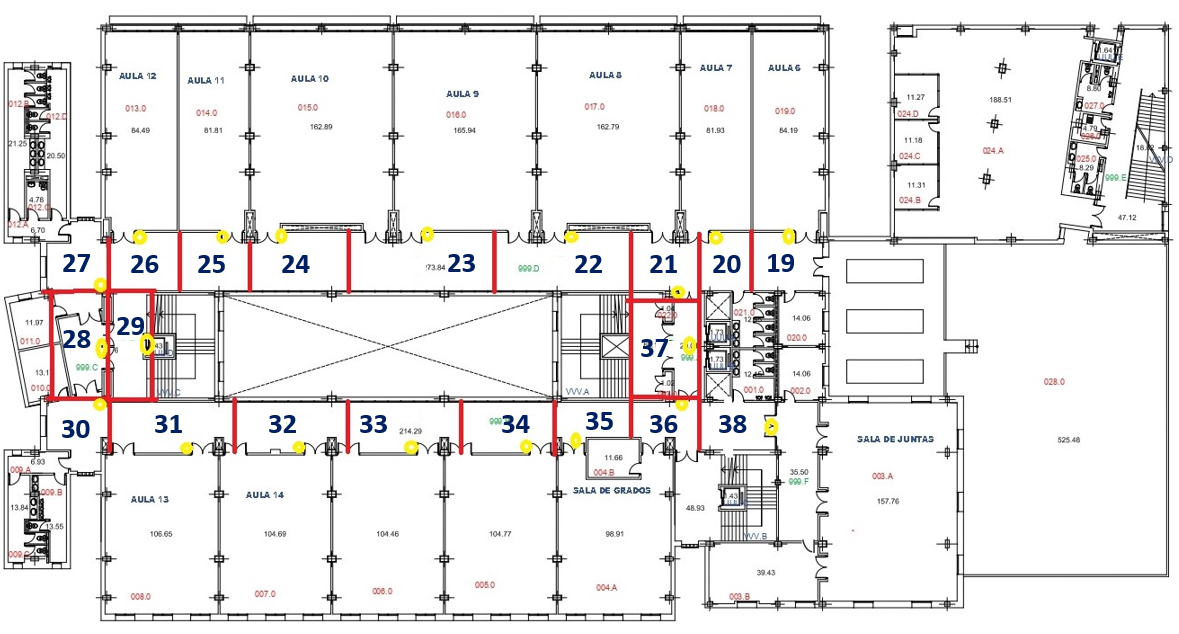
\includegraphics[width=1\textwidth]{Imagenes/Descripciondeltrabajo/mapeoPlanta1}
	\caption{Versión final del mapeo de la primera planta de la Facultad de Informática.}
	\label{fig:cuadrantesP1_v3}
\end{figure}


Como nuestro posicionamiento se fundamenta en el \textit{beacon} más cercano, hemos considerado que el usuario se encuentra en el cuadrante asociado a dicho \textit{beacon}, de esta manera es como hemos relacionado la frase ``encontrarse en las inmediaciones de un \textit{beacon}'' con un punto del mapa. Sin embargo, por este mismo motivo, aquellos cuadrantes que no tienen asociada ninguna baliza bluetooth carecen de interés ya que no hay manera de detectarlos y saber si el usuario se encuentra en ellos. Es por esto que el siguiente cambio ha sido juntar ciertos cuadrantes formando unos nuevos más grandes. En la Figura \ref{fig:cuadrantesP1_v3} encontramos la versión final del mapeo, en la que solo permanecen los cuadrantes con baliza. Además podemos observar que también hemos suprimido los cuadrantes de las aulas, sala de juntas, etc. esto se debe a que nuestra aplicación no ofrece una guía dentro de estas estancias sino que funciona como guía de puerta a puerta. Por ello, en lugar de tener cuadrantes que se unen formando estancias hemos realizado el cambio a cuadrantes que se agrupan en plantas.

\begin{figure}[t]
	\centering
	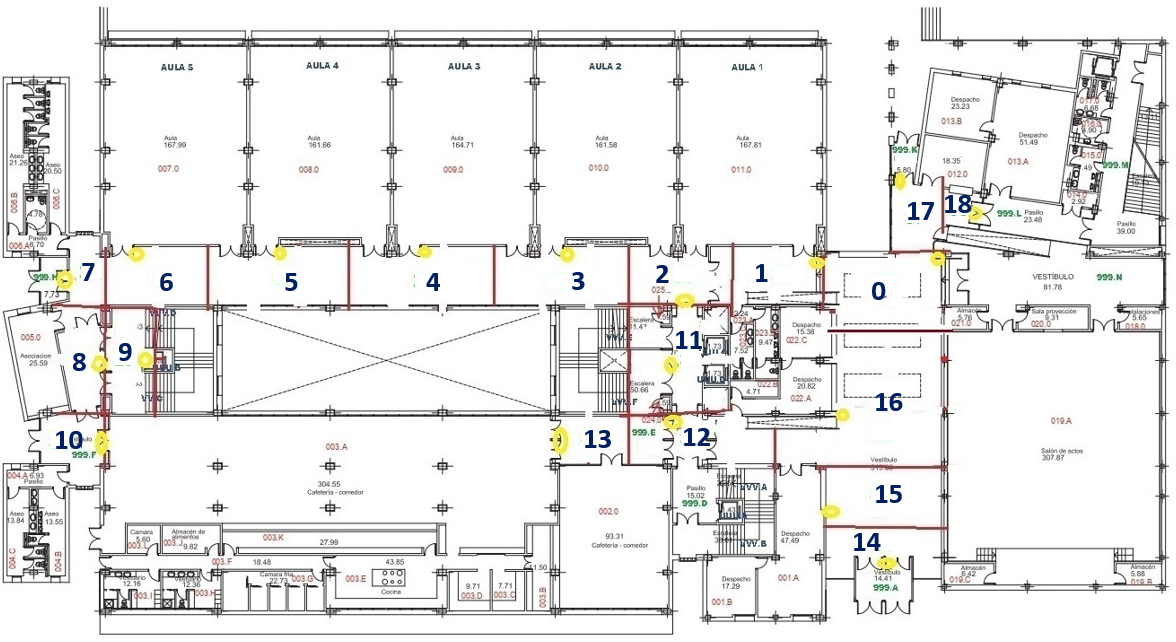
\includegraphics[width=1\textwidth]{Imagenes/Descripciondeltrabajo/mapeoPlantaBaja}
	\caption{Mapeo de la planta baja de la Facultad de Informática, incluyendo la numeración de los cuadrantes y las posiciones de los \textit{beacons}.}
	\label{fig:cuadrantesPbaja}
\end{figure}

La novedad más importante que incluye nuestro proyecto con respecto a los trabajos predecesores en este aspecto es el mapeo de la planta baja (ver Figura \ref{fig:cuadrantesPbaja}) y la conexión de unas plantas con otras a través de los cuadrantes en los que se encuentran los ascensores y escaleras de manera que sea viable incluir rutas de una a otra.



\section{Mediciones y distribución de los \textit{beacons} en la Facultad de Informática}
\label{sec:medicionesbeacons}

Ahora que hemos superado la primera barrera tecnológica y tenemos una idea más clara del mapeo, nos disponemos a dar el siguiente paso hacia la resolución del problema del posicionamiento. En este apartado proponemos una posible disposición de los \textit{beacons} en la Facultad de Informática de la UCM, para ello explicamos qué puntos hemos empezado considerando como puntos de decisión y su evolución hasta formar la disposición final que aparece en las Figuras \ref{fig:cuadrantesP1_v3} y \ref{fig:cuadrantesPbaja} como consecuencia de una serie de mediciones.

Antes de nada vamos a definir qué es un punto de decisión: Los puntos de decisión son aquellos lugares en los que el usuario requerirá la siguiente instrucción bien porque se ha creado incertidumbre (intersección de caminos), porque ha pasado mucho tiempo de la última instrucción (recta muy larga) o bien porque ha llegado al destino y requiere confirmación. Los puntos de decisión que hemos considerado en la Facultad de Informática son: los destinos (aulas, cafetería, biblioteca, conserjería, secretaría, salón de actos, sala de juntas, sala de grados, etc.), las intersecciones de caminos, los ascensores y escaleras, y las puertas de entrada o salida del edificio.

En la Figura \ref{fig:medidasPPrimera} mostramos visualmente los puntos de decisión que inicialmente hemos considerado (círculos rojos) en uno de los pasillos principales de la primera planta y los puntos desde los cuales hemos llevado a cabo las mediciones (cruces verdes). Esta estructura se repite tanto en la misma planta como en la planta baja por lo que las decisiones tomadas han sido las mismas y la evolución de la ubicación de los \textit{beacons} hasta ocupar su posición final ha sido copiada sin realizar pruebas distintas.

De manera análoga, en la Figura \ref{fig:medidasPBaja} mostramos la ubicación inicial de los \textit{beacons} en la zona del \textit{hall} de la planta baja y los puntos desde los cuales se han realizado las mediciones. El objetivo de todas estas mediciones es conocer la ubicación óptima de los \textit{beacons} para que a nuestro paso cerca de ellos, la distancia registrada sea lo más precisa posible y no sufra muchas interferencias. Este estudio debe ser especialmente exhaustivo en las zonas más delicadas, como las intersecciones o los lugares en los que se acumulan varios puntos de interés y que por ente, son más susceptibles a sufrir interferencias procedentes de otros \textit{beacons}. En la Sección X se pueden ver los resultados de estas mediciones. 
%RAQUEL DICE QUE PONGAMOS AQUI LOS RESULTADOS-BELENCHU!


\begin{figure}[t]
	\centering
	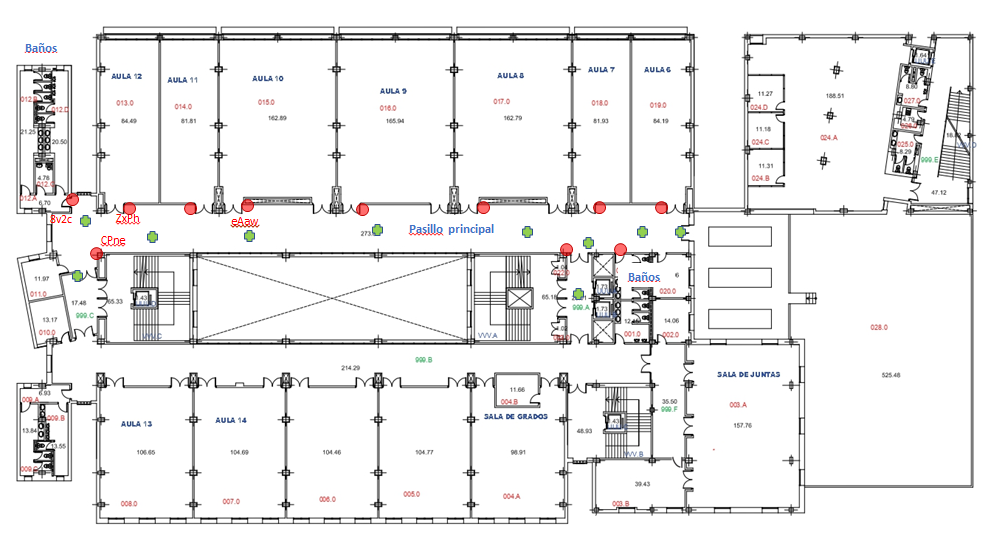
\includegraphics[width=1\textwidth]{Imagenes/Descripciondeltrabajo/mapa_mediciones_planta1}
	\caption{Mapa de la primera planta de la Facultad de Informática con la ubicación de los beacons (rojo) y los puntos de medición (verde). }
	\label{fig:medidasPPrimera}
\end{figure}

\begin{figure}[!h]
	\centering
	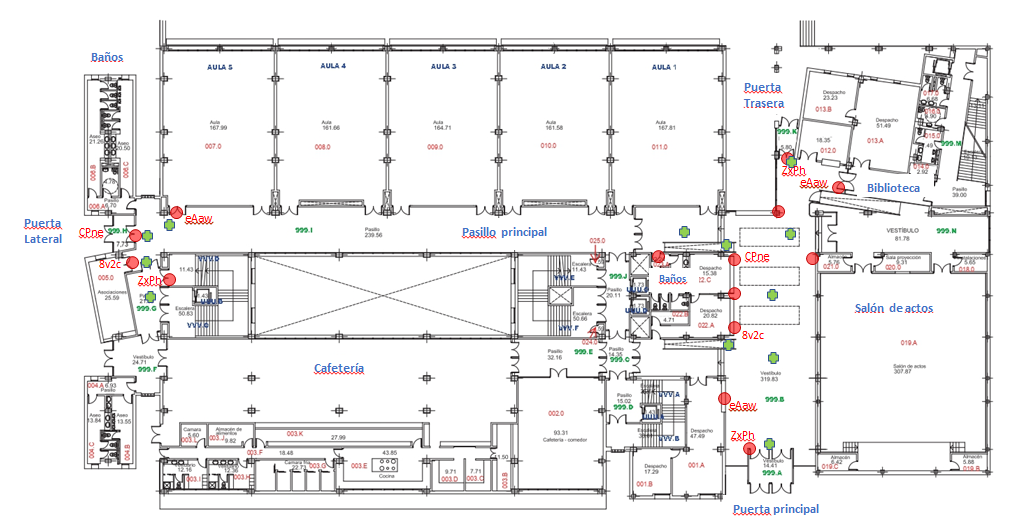
\includegraphics[width=1\textwidth]{Imagenes/Descripciondeltrabajo/mapa_mediciones_plantabaja}
	\caption{Mapa de la planta baja de la Facultad de Informática con la ubicación de los beacons (rojo) y los puntos de medición (verde). }
	\label{fig:medidasPBaja}
\end{figure}


A continuación exponemos las conclusiones obtenidas tras el estudio de los resultados:
\begin{itemize}
	\item Los \textit{beacons} no deben situarse demasiado cerca ya que las señales interfieren entre sí y alteran las distancias no pudiendo distinguir cuál es el \textit{beacon} más cercano. Por este motivo, hemos acordado no poner, por el momento, balizas en los baños ya que, tanto en la primera planta como en la planta baja, se encuentran en zonas repletas de puntos de interés. Para informar de la presencia de los baños y otras zonas de interés se desarrollará una funcionalidad que al pasar cerca de ellos te avisará de su presencia.
	
	\item En lugares diáfanos, como el \textit{hall}, la señal de los \textit{beacons} fluye con mayor libertad ya que no se encuentra con obstáculos. Es por esto, que deben situarse a mayor distancia entre sí. Uno de los problemas que se ha derivado de este hecho es cómo cubrir dicho espacio. Inicialmente colocamos una baliza en conserjería, otra en la intersección superior con el pasillo principal, otra en la intersección inferior con el pasillo que conduce a cafetería y otra enfrente para indicar la entrada al salón de actos (ver Figura \ref{fig:medidasPBaja}). Tras numerosas mediciones, la solución que proponemos es colocar las balizas de modo que una pueda servir para cubrir dos o más puntos de interés. Consecuentemente, hemos suprimido el \textit{beacon} de conserjería y hemos dejado exclusivamente el de las intersecciones ya que la inferior está muy próxima a la ventanilla de conserjería y puede reutilizarse para los dos puntos clave, y hemos desplazado un poco hacia arriba el \textit{beacon} del salón de actos para que sirva tanto para marcar dicho destino como para marcar la esquina superior que conduce hacia la biblioteca. En la Figura \ref{fig:beaconsPBaja} se puede ver el resultado final.
	
	\item Hemos hecho pruebas con los \textit{beacons} sobre distintas superficies y hemos comprobado que efectivamente el material puede alterar la señal. Particularmente, en el caso de las mediciones de la puerta lateral del edificio (lado izquierdo del mapa) hemos colocado el \textit{beacon} CPne justo encima de la puerta, en un bisel metálico que sobresale. El resultado ha sido que la señal de la baliza se proyecta con mayor intensidad, dando lugar a que la distancia estimada sea menor. Es decir, la aplicación sugiere que CPne está más cerca de lo que en realidad está. Tras esto, hemos concluido que lo óptimo es poner los \textit{beacons} sobre las mismas superficies, a ser posible no metálicas, y a la misma altura para que estén en igualdad de condiciones. 
	
	\item La última puntualización que hemos hecho tras las mediciones es que los \textit{beacons} de las intersecciones deben situarse en un punto lo más neutro posible ya que, al menos, se puede llegar desde dos puntos distintos y la señal se debe recibir de manera simétrica. 
\end{itemize}




\begin{figure}[t]
	\centering
	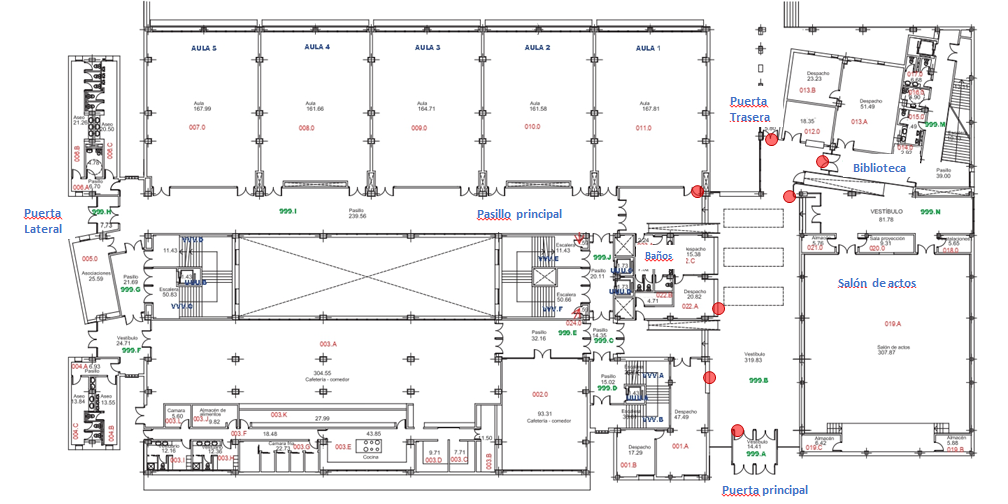
\includegraphics[width=1\textwidth]{Imagenes/Descripciondeltrabajo/beacons_plantabaja_final}
	\caption{Mapa de la planta baja de la Facultad de Informática con la ubicación definitiva de los beacons (rojo) en el hall. }
	\label{fig:beaconsPBaja}
\end{figure}

Este estudio no ha sido todo lo extenso que nos hubiese gustado debido al cierre de la Facultad de Informática a causa del COVID-19.

En el próximo apartado veremos cómo queda reflejado todo el mapeo visto en la Sección \ref{sec:mapeo}.

\section{Representación del mapeo en los XML}
\label{sub:mapeo_xml}
Todo nuestro mapeo se representa en ficheros XML que hemos sacado fuera de la aplicación (se encuentran en una carpeta llamada xml\_modif). En ellos hemos seguido el sistema de divisiones y estructuración del proyecto de TFG \textit{Generador interactivo de instrucciones de guía sobre plataformas móviles} \citep{TFGguia}, este permite que se puedan incluir
de manera sencilla las diferentes plantas del edificio y es un método genérico, lo que facilita que pueda ser empleado también por otros edificios. El sistema descrito se compone de ficheros de dos tipos:

\textbf{Edificio.xml:} En este archivo se guarda la información relativa a la estructura del edificio, es decir, se indican las distintas plantas y el archivo xml asociado a cada una de ellas. A continuación detallamos el significado de cada campo y vemos un ejemplo de la estructura del archivo.

\begin{itemize}
	\item \textit{nombre:} Nombre representativo de la planta que estemos implementando. En el ejemplo se ha utilizado el valor \textit{plantabaja} y \textit{planta1}.
	
	\item \textit{archivo:} Nombre del fichero xml de la planta en cuestión. No es necesario añadir la extensión .xml. En el ejemplo lo hemos llamado \textit{plantabajaarchivo} y \textit{planta1archivo}.
\end{itemize}

%\begin{figure}[t]
%	\centering
%	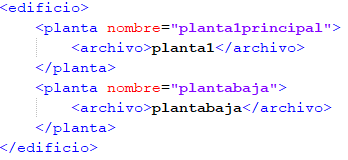
\includegraphics[width=0.7\textwidth]{Imagenes/Descripciondeltrabajo/edificioXML}
%	\caption{Ejemplo de un archivo con la misma estructura que edificio.xml.}
%	\label{fig:xmledificio}
%\end{figure}


\lstinputlisting[language=XML]{Imagenes/Descripciondeltrabajo/edificio.xml}

%\begin{figure}[t]
%	\centering
%	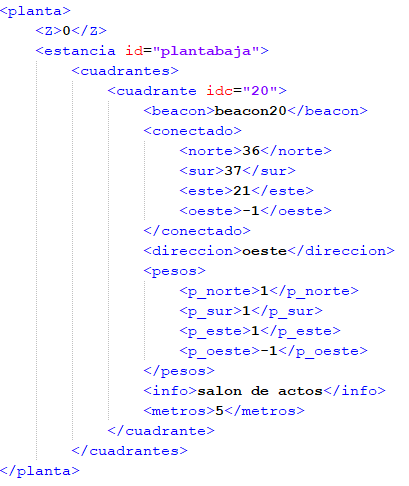
\includegraphics[width=0.7\textwidth]{Imagenes/Descripciondeltrabajo/plantaXML}
%	\caption{Ejemplo de un archivo que detalla la estructura de una planta.}
%	\label{fig:xmlplanta}
%\end{figure}

\textbf{NombreFichero.xml:} Se corresponde con el archivo propio de cada planta. Cada planta incluye un valor que indica el número de planta en el que nos encontramos y un identificador de estancia que da nombre a la planta y que agrupa al conjunto de cuadrantes que la forman. A su vez, cada cuadrante contiene un identificador único, el nombre del \textit{beacon} asociado, información sobre los cuadrantes colindantes, la posición en el cuadrante donde se encuentra el punto de interés (norte, sur, este u oeste), información sobre los pesos que tiene cada una de sus conexiones (cuya utilidad se presenta en la Sección \ref{sub:rutaOptima}), información relevante del cuadrante y la medida en metros del mismo. A continuación detallamos el significado de cada campo y vemos un ejemplo de la estructura del archivo.

\begin{itemize}
	\item \textit{Z:} Indica el número de planta. En el ejemplo le hemos dado el valor $0$.
	
	\item \textit{id:} Se corresponde con el nombre de la planta en la que nos encontramos. En el ejemplo la hemos llamado \textit{plantabaja}.
	
	\item \textit{idc:} Hace referencia al identificador único de cada cuadrante. En el ejemplo le hemos dado el valor $20$.
	
	\item \textit{beacon:} Hace referencia al identificador de la baliza asociada a dicho cuadrante. En el ejemplo le hemos dado el valor \textit{beacon0}.
	
	\item \textit{conectado:} Indica los identificadores de los cuadrantes colindantes por los cuatro puntos cardinales. El valor $-1$ representa la pared. Este campo ha sido reutilizado de trabajos anteriores ya que resulta clave para establecer una red de cuadrantes que nos permita generar una ruta válida pasando a través de ellos.
	
	\item \textit{posdestino:} Nos indica en qué posición del cuadrante está situado el punto de interés. En nuestro caso es el salón de actos, correspondiente al cuadrante $0$, como se puede ver en la Figura \ref{fig:cuadrantesPbaja} el salón de actos se sitúa al lado derecho del cuadrante (oeste)\footnote{La nomenclatura se establece con el sur en la parte de arriba, el oeste a la derecha, el norte abajo y el este a la izquierda del cuadrante.}.
	
	\item \textit{pesos:} Para cada una de las conexiones del cuadrante se establece el peso de dicha conexión. Esto será de gran utilidad pues el algoritmo utilizado para el cálculo de la ruta es el algoritmo de \textit{Dijkstra}. Los detalles pueden verse en la Sección \ref{sub:rutaOptima}. Los pesos negativos se asignan a conexiones inexistentes.
	
	\item \textit{info:} Este campo contiene la información relevante del cuadrante. La utilidad e importancia de este campo radica en informar al usuario, si lo desea, de qué hay a su paso por la ruta hasta el destino seleccionado. Esta idea nació tras la reunión en la ONCE en la que nos acercamos mucho a las necesidades de nuestros usuarios. En el ejemplo le hemos dado el valor \textit{salon de actos}.
	
	\item \textit{metros:} Este campo contiene la medida en metros del cuadrante lo que aporta mucha precisión a las instrucciones. En el ejemplo le hemos dado el valor $5$.
\end{itemize}


\lstinputlisting[language=XML]{Imagenes/Descripciondeltrabajo/planta.xml}


\chapter{Diseño e implementación}
\label{cap:diseñoeimplementación}


En este capítulo abordaremos los detalles técnicos de nuestra aplicación Blind Bit. Esta aplicación está diseñada como un modelo cliente-servidor, en la que el cliente (dispositivo móvil) se encarga de solicitar los datos necesarios (origen, destino, posición actual, etc.) al usuario para enviárselos al servidor, quien calcula la ruta y responde con la guía correspondiente. De esta manera, nuestra aplicación está mejor organizada, es más eficiente y evita que los dispositivos móviles se queden sin batería rápidamente a causa de una pesada carga computacional.

Al igual que la aplicación, este capítulo se divide en dos partes. La primera de ellas, Sección \ref{sec:servidor}, expone el funcionamiento general del servidor (Sección \ref{sub:func_servidor}) así como la implementación de sus dos funcionalidades principales: el cálculo de la ruta óptima (Sección \ref{sub:rutaOptima}) y la generación de instrucciones (Sección \ref{sub:genInstruc}). La segunda, Sección \ref{sec:cliente}, se centra en la implementación y el diseño de la aplicación móvil. En la Sección \ref{sub:diseño} revisamos la interfaz de la aplicación y la justificación de su diseño, mientras que en la Sección \ref{sub:func_cliente} nos adentramos en su funcionamiento desde el punto de vista técnico. Por último, en la Sección \ref{sec:adaptacion} se detallan los cambios pertinentes para desplegar la aplicación en un edificio distinto a la Facultad de Informática de la UCM.



\section{Servidor}
\label{sec:servidor}
El servidor constituye una parte indispensable del proyecto ya que se encarga de realizar los cálculos más pesados para no sobrecargar al dispositivo móvil. Sus principales funcionalidades son:
\begin{itemize}
	\item Almacenar la estructura e información referente al edificio mapeado.
	\item Permanecer a la escucha de cualquier cliente que solicite conexión.
	\item Solventar el posicionamiento del cliente conectado.
	\item Generar la ruta óptima desde la posición actual hasta el destino indicado por el cliente.
\end{itemize} 

La aplicación servidor está diferenciada en dos partes: el código escrito en lenguaje Java y los archivos correspondientes al edificio que se mapea, en nuestro caso la Facultad de Informática de la UCM. Estos archivos son los XML mencionados en la Sección \ref{sec:mapeo} y un archivo json que contiene la información referente a los distintos cuadrantes asociados a los destinos considerados por nuestra aplicación (por ejemplo, secretaría, conserjería, cafetería, las aulas,  etc.). 
Buena parte del código que conforma el servidor ha sido reutilizado de trabajos anteriores, concretamente de los proyectos de TFG \textit{Generador interactivo de instrucciones de guía sobre plataformas móviles} \citep{TFGguia} y del proyecto \textit{Sistema de guía por voz en interiores} \citep{TFGMariana}. La estructura de nuestro servidor se corresponde con la de \cite{TFGguia}. Sin embargo, hemos introducido cambios notorios para el desarrollo de esta aplicación que comentaremos a continuación.

\subsection{Funcionamiento del servidor}
\label{sub:func_servidor}

Para entender mejor la estructura del servidor, haremos un recorrido desde la carga de la información procedente de los archivos XML que representan el mapeo del edificio hasta la conexión con el cliente y el cálculo de la ruta: 


\begin{figure}[t]
	\centering
	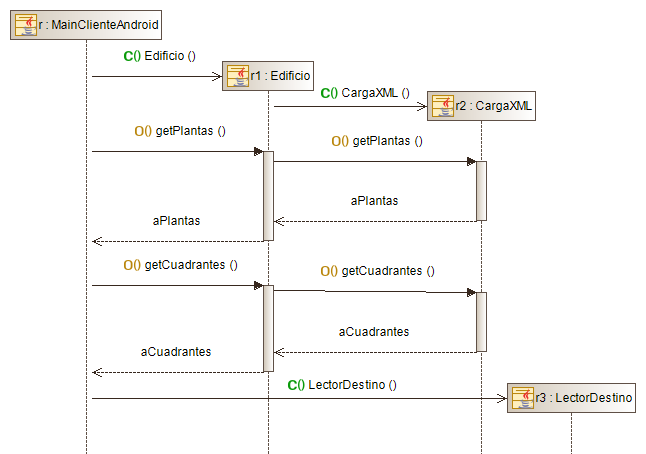
\includegraphics[width=0.8\textwidth]{Imagenes/Capitulo4/diagramasUML/arranqueServidor}
	\caption{Diagrama de secuencia para el arranque del servidor.}
	\label{fig:diag_sec_arranqueServ}
\end{figure}



\begin{itemize}
	\item \textit{Arranque del servidor:} Cuando el servidor arranca es necesario que guarde la información relativa al edifico para que pueda almacenar su estructura y generar una ruta válida para proporcionársela al cliente que la solicita. Al igual que los XML, el código relacionado con la carga de estos archivos, que conforma las clases \textit{CargaXML} y \textit{Edificio}, también se apoya en el del proyecto de \cite{TFGguia} ya mencionado en otras ocasiones. Estas clases permiten cargar los archivos y almacenar la información referente a los cuadrantes estructurada en plantas. En la Figura \ref{fig:diag_sec_arranqueServ} puede verse el diagrama de secuencia correspondiente a las explicaciones que siguen.
	
	Para nuestro trabajo se han añadido los atributos de clases necesarios para guardar la información nueva incluida en los XML (como los \textit{beacons}, los metros que ocupa el cuadrante, los pesos asociados a las conexiones, la ubicación del punto de interés o la información relevante de este) y se han eliminado aquellas que ya no se utilizan (como las coordenadas sureste y noroeste que no están presentes en nuestro proyecto). Una vez que está cargada esta información y ya tenemos la lista de cuadrantes existentes, pasamos a generar la matriz de adyacencia de la clase \textit{ListaCuadrantes} con la que representamos el mapa en forma de grafo y establecemos las conexiones entre cuadrantes. Esta tarea es relativamente sencilla, pues los XML nos proporcionan la información sobre los cuadrantes colindantes. El cambio más notorio que se ha introducido en este punto es dotar a las conexiones de la matriz de adyacencia de determinados pesos según la adaptabilidad de la ruta a nuestros usuarios objetivo. Estos cambios aparecen explicados con detalle en la Sección \ref{sub:rutaOptima}. 
	
	Es en este momento inicial cuando el servidor también carga el archivo \textit{destinos.json} con la lista de destinos y los cuadrantes asociados correspondientes. Una de sus entradas es, por ejemplo: \{``lugar'': ``aula 5'', ``cuadrante'': ``6''\}. En la clase \textit{LectorDestino} (reutilizada del proyecto de TFG \citep{TFGguia}) se almacenan cada una de las entradas en una tabla hash que cuenta con un campo clave de tipo String y un campo valor de tipo Integer que relaciona el lugar con su cuadrante asociado. 
	
	
	
	\item \textit{Conexión con el cliente:} Una vez que el servidor ha almacenado toda la información correspondiente al edificio, está preparado para recibir peticiones de los clientes. El servidor queda entonces a la espera de los clientes en la clase \textit{MainClienteAndroid}, escuchando a través de un \textit{webSocket} en un puerto determinado. Esta conexión cliente-servidor constituye otro de los cambios principales realizados con respecto a \cite{TFGguia}, pues se ha reestructurado por completo. En primer lugar, la conexión ya no se hace por medio de \textit{sockets} sino por medio de \textit{webSockets}. Esto implica una mayor seguridad en el intercambio de mensajes (se emplea el protocolo http) y permite que el código del servidor pueda ser utilizado como servidor externo. En nuestro caso hemos montado el servidor sobre una máquina virtual con una IP pública de la Facultad de Informática utilizando TomCat\footnote{\url{http://tomcat.apache.org/}}. Esto permite que los clientes puedan acceder al servidor desde cualquier red, lo cual es primordial para poder establecer conexión con el servidor desde la propia Facultad, en particular. En segundo lugar, el número de conexiones que tiene que establecer el cliente con el servidor para obtener la información necesaria de la ruta se ha optimizado al máximo. En un solo mensaje el servidor envía al cliente toda la información necesaria para seguir una ruta completa. En el proyecto que hemos tomado como modelo, el cliente, en cambio, debía solicitar al servidor una nueva instrucción cada vez que actualizaba su posición. Ahora el cliente hace una única petición indicando su \textit{beacon} más cercano (que se tomará como origen) y el destino al que quiere ir, en un mensaje del tipo \textit{IDdelBeaconOrigen$|$destino}, por ejemplo ``\textit{CPne$|$aula 8}''. Cuando el servidor recibe este mensaje, se encarga de generar la ruta desde el origen hasta el destino y enviársela al cliente. La información que se envía está compuesta por la lista de \textit{beacons} asociados a los cuadrantes que conforman la ruta desde el origen hasta el destino, las instrucciones necesarias, una lista de \textit{booleanos} que indican cuándo hay que hacer un giro en la ruta y su dirección (izquierda o derecha), y la información adicional de los cuadrantes que conforman la ruta. Por ejemplo, para la petición del cliente \textit{beacon14$|$aula 3}, donde suponemos que \textit{beacon14} se encuentra en el cuadrante $14$ y que el aula 3 es el cuadrante 4 (ver Figura \ref{fig:ruta_optima}, línea verde), obtendríamos el mensaje que vemos en la Figura \ref{fig:ejemplo_ruta}. La lista de \textit{beacons} se representa en verde con un centinela FINAL que indica que en el \textit{beacon4} se termina la ruta, y la lista de instrucciones a seguir en azul, separadas por el carácter @ atendiendo al cuadrante al que pertenecen. Debido a la imposibilidad de ir a la Facultad de Informática a causa de la COVID-19 se ha supuesto que todos los cuadrantes miden cinco metros, aunque esta información no se corresponde con la realidad. En morado se representa el cuadrante en el que hay que girar y la dirección. Como vemos, el ``iz'' corresponde al cuadrante $0$, que es en el que hay que hacer el giro a la izquierda (para el giro a la derecha el string asociado es ``der''). Por último, en gris se presenta la información adicional de cada cuadrante, donde un ``no'' indica que no hay información asociada a dicho cuadrante.
	
	\begin{figure}[t]
		\centering
		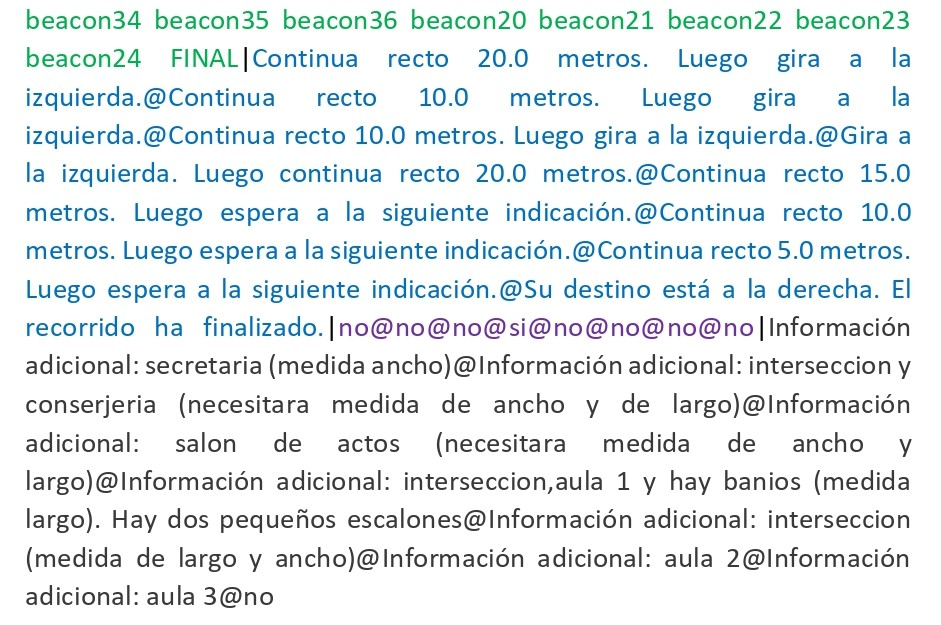
\includegraphics[width=0.9\textwidth]{Imagenes/Capitulo4/ejemploRuta}
		\caption{Ejemplo de la información generada por el servidor para una ruta desde el cuadrante $14$ al $4$.}
		\label{fig:ejemplo_ruta}
	\end{figure}
	
	  
	\item \textit{Generación de la ruta:} Esta funcionalidad es la más importante del servidor. El objetivo es obtener toda la información referente a la ruta desde el origen al destino seleccionado (ver Figura \ref{fig:ejemplo_ruta}). Lo primero que hay que hacer es obtener los cuadrantes origen y destino. Recordemos que lo que tenemos es el \textit{beacon} más cercano al cliente y el destino como cadena de caracteres (String), pero se desconoce a qué cuadrantes corresponden. Para ello, se busca el cuadrante asociado al \textit{beacon} y al destino recorriendo la lista de cuadrantes del edificio (\textit{aCuadrantes}) y solicitando el valor asociado al destino (clave) en la tabla hash (\textit{lectorDest}). Con esta asociación entre \textit{beacons}/destinos y cuadrantes se resuelve el problema del posicionamiento. 
	
	Una vez se tienen los puntos que determinan la ruta se genera la lista de cuadrantes y de \textit{beacons} correspondientes mediante la función \textit{calculaRuta}. Esta está basada en el algoritmo de \textit{Dijkstra} (que reemplaza a la búsqueda en anchura utilizada en el proyecto de \cite{TFGguia}) que tiene como entrada la matriz de adyacencia de los cuadrantes (en la Sección \ref{sub:rutaOptima} pueden verse algunos detalles). Una vez que tenemos la lista de cuadrantes por los que el usuario debe pasar hasta llegar al destino se generan las instrucciones necesarias para guiar al usuario. Este es el cometido principal de la función \textit{generar}. Esta función tiene como entradas el cuadrante actual (en el que se encuentra el usuario), que se va simulando mediante un bucle, y el destino, y en función de los cuadrantes de la ruta, más concretamente de los inmediatos al cuadrante actual, construye la siguiente instrucción (ver detalles en la Sección \ref{sub:genInstruc}). En la Figura \ref{fig:diag_sec_conexionYRutaServ} puede verse el diagrama de secuencia.	Cuando se ha llamado a \textit{generar} con todos los cuadrantes que conforman la ruta, ya se tiene la lista de instrucciones completa y se contesta al cliente. 
\end{itemize}




\begin{figure}[t]
	\centering
	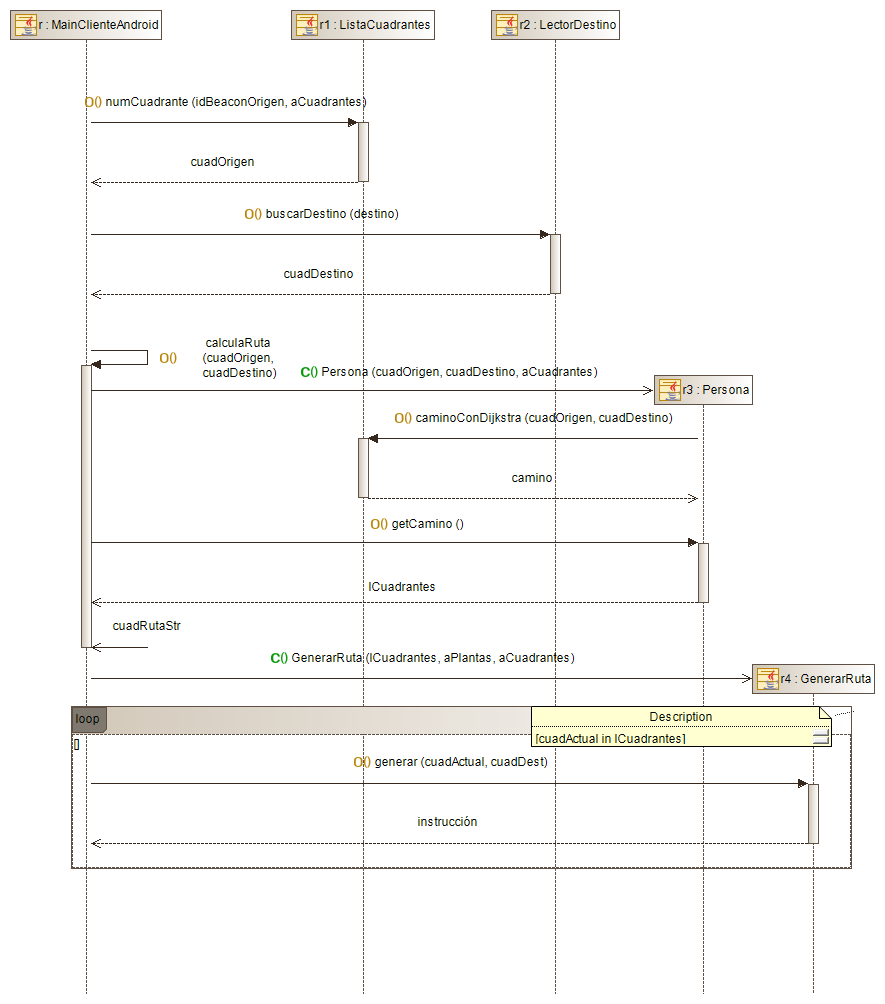
\includegraphics[width=0.8\textwidth]{Imagenes/Capitulo4/diagramasUML/generacionRuta}
	\caption{Diagrama de secuencia para la generación de la ruta.}
	\label{fig:diag_sec_conexionYRutaServ}
\end{figure}



\subsection{Cálculo de la ruta óptima}
\label{sub:rutaOptima}

En esta sección veremos las modificaciones que se han hecho para lograr guiar al usuario por la ruta más conveniente. Como ya hemos mencionado anteriormente, el mapeo nos proporciona un grafo en el que los cuadrantes son los nodos y las conexiones entre ellos, las aristas. Para su representación hemos empleado una matriz de adyacencia y de esta manera el cálculo de la ruta más corta entre dos cuadrantes se reduce al algoritmo de \textit{Dijkstra}.

Sin embargo, no debemos olvidar que nuestra aplicación tiene un usuario final muy concreto: personas con discapacidad visual. Es por ello que la ruta debe ser lo más sencilla posible, libre de obstáculos y otros elementos que puedan entorpecerlos, por lo que en ocasiones la ruta óptima no coincide con la más corta sino con la que esté mejor adaptada. Para representar esta adaptabilidad, a aquellas conexiones que presenten una mayor dificultad para las persona invidentes se les ha asignado un peso mayor en la matriz de adyacencia (ver Sección \ref{sub:mapeo_xml}), a fin de buscar este equilibrio entre la ruta más corta y la más adecuada. En la Figura \ref{fig:ruta_optima} aparece un ejemplo de esta situación: si quisiéramos ir desde la puerta principal (cuadrante $14$) al aula 3 (cuadrante $4$), el camino más corto implicaría pasar por delante de los ascensores (ruta roja). Sin embargo, la conexión entre los cuadrantes $12$ y $11$, y $11$ y $2$ puede resultar tediosa para una persona invidente. Las razones que hemos considerado son: 
\begin{itemize}
	\item El tramo compuesto por los cuadrantes $12$, $11$ y $2$ es más estrecho que su camino paralelo por el \textit{hall}.
	\item Presenta más giros e intersecciones de caminos.
	\item Normalmente acumula más gente ya que es zona de paso para coger los ascensores o subir/bajar por las escaleras o entrar/salir de la cafetería.
\end{itemize} 
 	Todo esto es potencialmente problemático en ausencia de la vista y considerando además que nuestros usuarios es probable que vayan acompañados de un perro guía o un bastón. Por ello, hemos concluido ajustar los pesos en la matriz de adyacencia y la ruta generada pasa a ser la señalada en verde. De esta manera limitamos el paso por el pasillo de los ascensores a aquellas rutas en las que es estrictamente necesario, es decir, cuando se requiere un cambio de planta. Este tipo de consideraciones se han tenido en cuenta en las distintas zonas del edificio que presentan este tipo de características.


\begin{figure}[t]
	\centering
	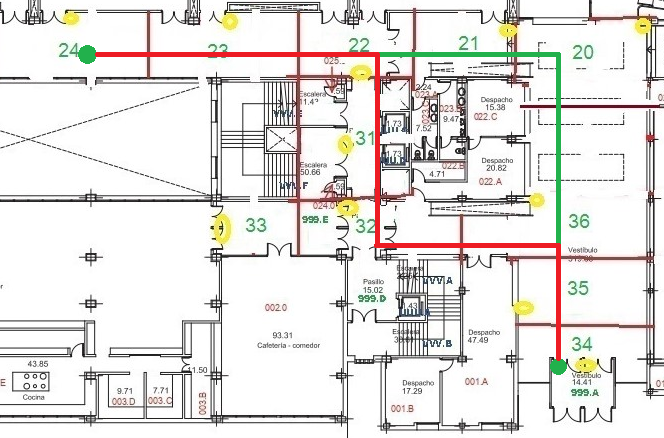
\includegraphics[width=0.8\textwidth]{Imagenes/Capitulo4/mapa_ruta_optima}
	\caption{Ejemplo de ruta óptima entre dos puntos.}
	\label{fig:ruta_optima}
\end{figure}

\subsection{Generación de instrucciones}
\label{sub:genInstruc}

La función que contiene toda la lógica relativa a la generación de las instrucciones es \textit{generar}. Esta función es una de las que más modificaciones ha sufrido con respecto a los trabajos predecesores, pues no solo la hemos adaptado para personas con discapacidad visual sino que también hemos incluido mucha complejidad procedente de los cambios de planta y demás casuística que no estaba previamente incluida. Algunas de las modificaciones son: 

\begin{itemize}
	\item Se ha añadido más precisión e información a las instrucciones. De esta manera, cuando el usuario llega al destino correspondiente la instrucción especifica dónde se encuentra este, por ejemplo ``Su destino está a la derecha (o a la izquierda o delante...)'' dependiendo de por dónde haya llegado el usuario (en la Sección \ref{sub:instr_giro} se detalla la implementación de esta funcionalidad). Otro caso en el que se ha añadido mayor precisión es al puntualizar los metros que el usuario debe continuar en una dirección dada. En la Figura \ref{fig:ejemplo_ruta} podemos ver un ejemplo de ruta en el que se especifica el número de metros que el usuario debe seguir recto hasta ejecutar el siguiente giro o la siguiente acción, y como a medida que el usuario va avanzando la distancia va disminuyendo. Esto favorece que el usuario reconozca que va en la dirección correcta y pueda calcular mejor cuando ha de girar o ejecutar cualquier otra acción. A diferencia de los trabajos predecesores, nuestra app proporciona una instrucción nueva en cada cuadrante, es decir, no se salta ninguno como sucedía en el caso de las rectas (pasillos) en el proyecto precedente. Esto se ha hecho así ya que por un lado hemos considerado cuadrantes más grandes y por tanto la distancia recorrida de un cuadrante a otro es mayor, y porque creemos muy conveniente que el usuario reciba de manera continuada \textit{feedback} por parte de la aplicación para cerciorarse de que va por el camino correcto y que la aplicación no ha dejado de funcionar. Finalmente, también se ha ajustado el orden de las instrucciones para proporcionarlas de manera correcta. Por ejemplo, si la instrucción siguiente es un giro se invierte el orden para indicar primero el giro y después los metros que debe continuar en la nueva dirección.
	
	
	\item Se han incluido cambios de planta, lo que supone una gran novedad respecto al proyecto de \cite{TFGguia}. Ahora los cuadrantes de distintas plantas correspondientes a los ascensores están unidos\footnote{El cuadrante $11$ (correspondiente a los ascensores situados detrás de conserjería) está conectado con el $37$ (ascensor correspondiente al anterior en la planta 1) y el $9$ (ascensor más cercano a la puerta trasera de la cafetería) con el $29$ (ascensor correspondiente al anterior en la planta 1).} permitiendo así que la lista de cuadrantes de la ruta esté formada por cuadrantes de distinta planta. La función \textit{generar} detecta cuando el siguiente cuadrante al que queremos ir no está en la misma planta que el de nuestra posición actual y genera la instrucción en consonancia ``Los ascensores están a tu izquierda. Sube a la primera planta'' o ``El ascensor está delante. Sube a la primera planta'', por ejemplo. También se tiene en cuenta en las instrucciones el caso particular de las zonas de ascensores, pues hay dos zonas por planta pero no son simétricas por lo que las instrucciones son distintas. Por ello, para salir de la zona de los ascensores correspondientes al cuadrante $11$ (los que se sitúan detrás de conserjería) debemos simplemente girar, mientras que para salir de los de la zona de la puerta trasera de la cafetería (cuadrante $13$) debemos caminar escasos metros hacia adelante y después girar. A pesar de que en la Facultad de Informática contamos con ascensores y escaleras, se ha supuesto que la ruta se seguirá por medio de los ascensores ya que de esta manera es más fácil el cambio de planta y, además, estos se encuentran adaptados con botones en \textit{braille}.
	
	\item Se ha añadido una funcionalidad que permite informar al usuario (si lo desea) sobre lo que se va encontrando a su paso por la ruta, véase los baños, la cafetería, el despacho de Delegación de Alumnos, unos escalones, etc. Esto es fundamental, pues además de proporcionar seguridad al usuario en su primera visita a un edificio, le da la opción de tener una mejor idea global del espacio en el que se encuentra. Para ello lo que se hace es incluir en la ruta la información contenida en el cuadrante siguiente al que se encuentra el usuario, y de esta manera conseguimos adelantarnos y avisar al usuario con antelación. Así mismo, la función \textit{generar} enviará información sobre cuándo el usuario deberá hacer un giro para permitir avisar a este de manera especial (con una vibración) desde la aplicación del cliente.
	
\end{itemize}

\begin{figure}[t]
	\centering
	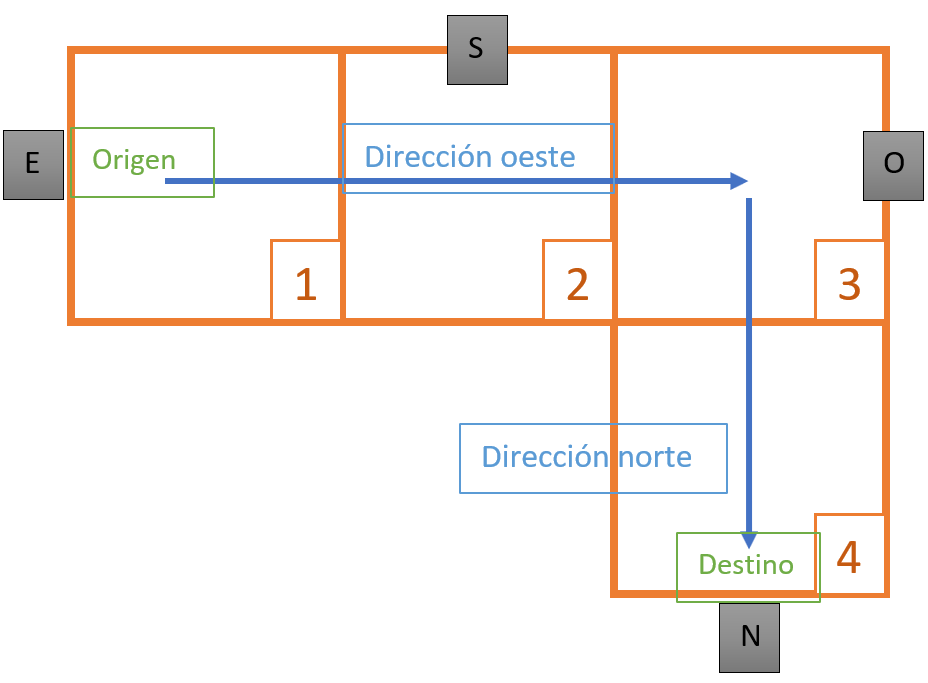
\includegraphics[width=0.8\textwidth]{Imagenes/Capitulo4/simulacion_giro}
	\caption{Ejemplo de giro en la ruta.}
	\label{fig:simulacion_giro}
\end{figure}


\subsubsection{Implementación de las instrucciones de giro}
\label{sub:instr_giro}

Como ya avanzábamos al comienzo de la sección anterior, la función que genera las instrucciones completas es \textit{generar}. Sin embargo, esta se apoya en la función \textit{indicaDirFinal}, cuya finalidad es indicar si se debe hacer un giro y, en ese caso, hacia qué lado. Esto resulta de gran utilidad tanto para saber hacia dónde debe dirigirse el usuario en caso de que tenga que hacer un cambio de dirección en su camino, como para poder indicarle dónde se encuentran ciertos puntos de interés durante la ruta (como los ascensores o el destino): si a su izquierda, a su derecha o delante.

La lógica de la función \textit{indicaDirFinal} es bastante sencilla. Esta toma como parámetro de entrada dos direcciones, la primera de ellas indica la dirección en la que vamos y la segunda la dirección a la que queremos llegar. En la Figura \ref{fig:simulacion_giro} se ilustra el ejemplo de una ruta con un giro. En este caso, la dirección en la que vamos sería el oeste (en gris se muestra la posición de los puntos cardinales de referencia). Al llegar al cuadrante $3$, la dirección que debemos tomar es norte, la cual no coincide con la dirección que llevábamos. Es entonces cuando la función \textit{generar} sabe que el usuario debe hacer un giro y llama a la función \textit{indicaDirFinal} con los parámetros oeste y norte, en ese orden. La lógica de \textit{indicaDirFinal} se basa en una serie de \textit{if-elses} que determinan las direcciones de giro correspondientes. En este caso en el cuadrante $3$ nos devolvería el giro a la derecha. Una vez que nos encontramos ya en el cuadrante $4$, \textit{generar} reconoce que es el cuadrante destino (pues este uno de sus parámetros de entrada) y, en función de dónde se sitúe el punto de interés de este cuadrante destino, indica al usuario dónde está con ayuda de la función \textit{indicaDirFinal}. En este caso sería \textit{su destino está delante}, pues no hay que realizar ningún cambio de dirección. 

\section{Cliente}
\label{sec:cliente}
En nuestro proyecto el cliente constituye la aplicación en sí misma. Esta la hemos bautizado como Blind Bit y ha sido desarrollada para Android. A través de ella el usuario solicita la ruta a un destino determinado, la aplicación conecta entonces con el servidor, que es quien la calcula, y se la reenvía al cliente. Finalmente, la aplicación se encarga de proporcionar, en el momento adecuado, las instrucciones necesarias para llegar al destino y utiliza sonidos y vibraciones para advertir de diferentes situaciones, como giros o aprobación de que seguimos en el camino correcto.

El cliente está desarrollado como un código genérico que es completamente independiente al edificio que se refiere. De esta manera, puede reutilizarse siempre que se incluya la información pertinente siguiendo el modelo que planteamos. La información a incluir es aquella relativa a la lista de destinos que la guía es capaz de reconocer y ha de ubicarse en el archivo XML \textit{listasStringsApp.xml}. En este archivo se encuentran los destinos con el mismo nombre que a su vez reconoce el servidor y que incluye respectivamente en el archivo \textit{destinos.json}, lo que permite que antes de conectar con el servidor podamos comprobar que el destino solicitado por el usuario es correcto. 

A continuación presentamos tanto los detalles de diseño de la aplicación como los detalles técnicos de su implementación.

\subsection{Diseño de la aplicación Blind Bit}
\label{sub:diseño}

A la hora de abordar el diseño de la aplicación hemos tenido muy presente el hecho de que nuestros potenciales usuarios finales son personas con discapacidad visual. Por ello hemos plateado interfaces sencillas y poco aglomeradas, en las que los botones sean lo más grandes posibles y estén bien organizados para que sea fácil de utilizar y memorizar. De esta manera, la mayor parte de los botones que hemos incluido tienen forma rectangular y ocupan todo el ancho de la pantalla, lo que favorece el uso de la app con ayuda del lector de pantalla. No solo hemos tenido en cuenta el lector de pantalla en la forma y el tamaño de los botones sino también a la hora de cambiar el nombre de cada pantalla especificando en cual se encuentra el usuario (por defecto aparecía el mismo nombre en todas) y en el hecho de evitar que este reproduzca todas las figuras que aparecen en la pantalla (modo por defecto) ya que sobrecarga al usuario proporcionándole información que en algunos casos carece de interés, como sucede con el logotipo de la app o ciertos cuadros de texto.

Por otro lado, hemos incluido algunas vibraciones y sonidos característicos con el fin de advertir al usuario de ciertas situaciones y acciones de manera no verbal. De esta manera, no saturamos al usuario con demasiada información extra pero le ayudamos en el uso de la app. Estos son: sonido de \textit{acierto} cuando el usuario completa correctamente la instrucción dada, una vibración larga en el momento en el que pasa por una intersección de caminos y ha de girar a la izquierda, dos vibraciones cortas cuando en cambio ha de girar a la derecha y tres cuando ha llegado a su destino.

A continuación describimos las pantallas de nuestra aplicación, que pueden verse en la Figura \ref{fig:interfaz}, y los detalles de su diseño:

\begin{figure}
	\def\tabularxcolumn#1{m{#1}}
	\centering
	\begin{tabularx}{\linewidth}{@{}cXX@{}}
		%
		\begin{tabular}{ccc}
			\subfloat[Pantalla principal]{\includegraphics[width=0.3\textwidth]{Imagenes/Capitulo4/PantallaPrincipal}} 
			& \subfloat[Pantalla de destinos]{\includegraphics[width=0.3\textwidth]{Imagenes/Capitulo4/PantallaListaDestinos}}
			& \subfloat[Pantalla de aulas]{\includegraphics[width=0.3\textwidth]{Imagenes/Capitulo4/PantallaListaAulas}}\\
			\subfloat[Pantalla de ruta]{\includegraphics[width=0.3\textwidth]{Imagenes/Capitulo4/PantallaRuta}} 
			& \subfloat[Pantalla instrucciones de uso]{\includegraphics[width=0.3\textwidth]{Imagenes/Capitulo4/PantallaInstrucciones1}}
			& \subfloat[Segunda pantalla instrucciones de uso]{\includegraphics[width=0.3\textwidth]{Imagenes/Capitulo4/PantallaInstrucciones2}}\\
			%\subfloat[E]{\includegraphics[width=0.3\textwidth]{Imagenes/Capitulo4/PantallaPrincipal}} 
			%& \subfloat[F]{\includegraphics[width=0.3\textwidth]{Imagenes/Capitulo4/PantallaPrincipal}}\\
		\end{tabular}
		%&
		%\subfloat[G]{\includegraphics[width=0.3\textwidth]{Imagenes/Capitulo4/PantallaPrincipal}}
		%&
		%\subfloat[H]{\includegraphics[width=0.3\textwidth]{Imagenes/Capitulo4/PantallaPrincipal}}
	\end{tabularx}
	
	\caption{Interfaz de la aplicación Blind Bit}\label{fig:interfaz}
\end{figure}

\begin{itemize}
	\item \textit{Pantalla principal:} En ella aparece el logo de la aplicación que ocupa el cuadro superior, y tres botones alargados que se sitúan en el cuadro inferior ocupando prácticamente todo el ancho de la pantalla. Los botones son, en orden descendente, \textit{Iniciar Ruta}, \textit{Ajustes} e \textit{Modo de uso} y están coloreados en lila, blanco y lila respectivamente para que aquellos usuarios que tienen visibilidad reducida puedan distinguir mejor cada botón. La finalidad de estos botones es muy intuitiva: el botón de \textit{Iniciar Ruta} nos conduce a una pantalla de destinos en la que podremos seleccionar uno para después comenzar la ruta hasta él; el botón de \textit{Ajustes} sirve para modificar algunos aspectos de la configuración como el volumen, el idioma de la aplicación, el tipo de voz que da las instrucciones, el modo de uso de la aplicación (que dé más información en las instrucciones o que sean más escuetas), etc; y por último, el botón de \textit{Modo de uso} conduce a una pantalla en la que se expone el modo de uso de la aplicación, con todas sus posibilidades.
	
	\item \textit{Pantalla de destinos:} Esta pantalla tiene como finalidad que el usuario seleccione el destino hasta el que quiere dirigirse para, tras ello, comenzar con la ruta. Debido al carácter especial de nuestros usuarios, hemos empleado un diseño que aporte distintas alternativas a esta búsqueda del destino, pues nuestro objetivo no es solo encontrar una vía que les resulte sencilla (como podría ser utilizar la app mediante voz) sino que también se amolde a distintas situaciones de la vida cotidiana (siguiendo con el mismo ejemplo, en determinadas circunstancias utilizar la app mediante voz puede ser molesto o causar vergüenza al usuario). Por ello, en el margen superior de la pantalla hemos situado una barra de escritura, que ocupa todo el ancho, en la que el usuario puede escribir directamente el nombre del destino al que desea ir. Si por el contrario prefiere utilizar la app mediante voz hemos incluido un micrófono en la parte central del margen inferior a través del cual el usuario puede indicar el destino en voz alta. El motivo por el cual hemos decidido colocar el micrófono en la parte inferior de la pantalla es que pese a que el lector de pantalla va barriendo de arriba a abajo y, por tanto, el micrófono queda el último, ocupa una posición cercana al dedo pulgar tanto de la mano derecha como de la izquierda (ya que se ha colocado en medio) y por ende, aunque al principio haya que esperar un poco más hasta que el lector lo encuentre, una vez que el usuario sepa donde está, el acceso será más sencillo y rápido. Además no hay ningún otro botón próximo, lo que facilita aún más el acceso. Finalmente, siguiendo el modelo de diseño de la aplicación \textit{Lazarillo}, vista en la Sección \ref{sec:appGuia} del Capítulo \ref{cap:estadoDeLaCuestion}, hemos incluido una cuadrícula con 9 botones (3 filas de 3 botones) en la zona centra, en la que aparecen todos los posibles destinos de la Facultad (\textit{Aulas}, \textit{Cafetería}, \textit{Biblioteca}, \textit{Salón de Actos}, \textit{Sala de Juntas}, \textit{Sala de Grados}, \textit{Consejería},\textit{ Puerta Principal}, \textit{Secretaría}). Esta tabla se genera dinámicamente organizándose en filas de 3 botones como máximo y teniendo tantas filas como sean necesarias para incluir todos los destinos leídos del archivo \textit{listasStringsApp.xml}. Los botones se colorean intercaladamente de lila y blanco para que aquellos usuarios que tienen visibilidad reducida puedan distinguir los límites de los botones por sus colores. 
	
	Si se selecciona el botón \textit{Aulas} aparece la misma pantalla con la única variante de que la cuadrícula generada hace referencia a las aulas leídas del mismo archivo (\textit{listasStringsApp.xml}). Como en el caso concreto de la Facultad de Informática hay 16 aulas, la tabla está formada por 5 filas con 3 botones en cada una y una última fila en la que solo hay un botón. El nombre de los botones que aparece en cada cuadrícula es configurable según el edificio. Si por el contrario se selecciona cualquier otro botón de destino (un aula concreta, la cafetería, la sala de juntas, etc.) o se indica el destino con alguna de las otras dos alternativas (barra de escritura o micrófono) aparece la pantalla de ruta.
	
	\item \textit{Pantalla de ruta:} Esta pantalla es la encargada de proporcionar las instrucciones de la ruta hasta el destino seleccionado. En ella aparece un cuadro de texto en la parte superior, en el que se van escribiendo las instrucciones a medida que se reproducen en voz alta y un botón con forma de altavoz situado encima del cuadro de texto en la parte derecha, que sirve para silenciar la reproducción de las instrucciones. Al pulsar sobre él cambia su aspecto físico y pasa a ser un altavoz con una cruz que nos indica su nuevo estado (\textit{mute}). De nuevo hemos tomado la decisión de no usar exclusivamente la vía oral con el fin de crear una aplicación que se adapte a diversas situaciones y usuarios (personas invidentes, personas con discapacidad pero que mantienen algún resto visual e incluso personas videntes que busquen una guía por la Facultad), y sea así, lo más inclusiva posible. Además del cuadro de texto, aparecen 4 botones alargados que ocupan el resto de la pantalla. Estos son \textit{Iniciar Ruta} que como su nombre indica sirve para comenzar una vez que se ha seleccionado el destino, \textit{Repetir Instrucción} cuya finalidad es volver a dar la última instrucción en caso de que no se haya escuchado bien, e \textit{Instrucciones Detalladas} que sirve para activar y desactivar, según el estado previo, la funcionalidad de incluir más información durante la ruta (indicar qué hay alrededor). Cuando se modifica el estado de este botón el lector de pantalla avisa del nuevo \textit{modo instrucciones detalladas activado} o \textit{modo instrucciones detalladas desactivado}. Y por último, \textit{Finalizar Ruta} que sirve para forzar la finalización de la ruta. Cuando se pulsa este botón o bien la flecha para ir hacia atrás aparece una ventana emergente que pide confirmación para finalizar. De esta manera nos aseguramos de que el usuario no ha pulsado sin querer. 
	
	Atendiendo de nuevo a esta diversidad de usuarios, hemos coloreado los botones \textit{Iniciar Ruta} e \textit{Instrucciones Detalladas} en lila para que aquellos que tienen visibilidad reducida puedan distinguir los botones por sus colores. Por otro lado, el motivo por el cual hay un botón de \textit{Iniciar Ruta} en lugar de empezar directamente con la reproducción de instrucciones una vez que el destino ha sido seleccionado, es que tras hacer varias pruebas con el lector de pantalla advertimos que las instrucciones y el \textit{talkback} se solapaban y se volvían ininteligibles.
	
	\item \textit{Pantalla de Modo de uso:} En esta pantalla aparece el logo de la aplicación centrado en el margen superior y a continuación cuatro botones formando una columna en los que se plantean algunas de las dudas más frecuentes sobre el uso de Blind Bit: \textit{Cómo iniciar una ruta}, \textit{Cómo buscar un destino}, \textit{En qué consiste Repetir Instrucción} y \textit{Qué son las Instrucciones Detalladas}. Al pulsar cualquiera de estos botones aparece una pantalla que nos recuerda al diseño de la pantalla de ruta, en ella hay un gran cuadro de texto que ocupa la mitad superior de la pantalla y tres botones colocados en forma de columna que ocupan la otra mitad. Estos botones son, en orden descendente, \textit{Reproducir}, \textit{Siguiente} y \textit{Anterior}. De esta manera, si pulsas el primer botón (\textit{Reproducir}) aparece la instrucción correspondiente al modo de uso seleccionado, escrita en el cuadro de texto y reproducida en voz alta. Para volver a escucharla basta con pulsar de nuevo este mismo botón. Por otro lado, si se quiere saber la instrucción siguiente o anterior siguiendo el orden indicado en la pantalla de Modo de uso, basta con pulsar el botón correspondiente (\textit{Siguiente} o \textit{Anterior}, respectivamente). Con respecto a las decisiones tomadas en el diseño de esta última pantalla, hemos colocado los botones en este orden ya que hemos considerado que \textit{Reproducir} será el más utilizado y por ello parece conveniente que esté arriba. Siguiendo con esta linea de pensamiento, parece que lo más lógico a continuación, es querer ir a la instrucción siguiente por lo que hemos colocado justo debajo dicho botón (\textit{Siguiente}) y por último, el botón \textit{Anterior} en caso de que querer volver a una instrucción previa. Por otro lado, al igual que en la pantalla de ruta las instrucciones no empiezan hasta que no se pulsa el botón \textit{Reproducir}. Esto se debe al mismo motivo que entonces, si se usa la app con ayuda del lector de pantalla y las instrucciones comienzan directamente, se producen solapamientos en las reproducciones y se vuelven ininteligibles.
\end{itemize}



\subsection{Funcionamiento del cliente}
\label{sub:func_cliente}
En esta sección veremos el funcionamiento de la aplicación desde la interacción con el usuario hasta la conexión con el servidor y gestión de la ruta. 

\begin{itemize}
	\item \textit{Interacción con el usuario}: Como ya hemos tratado en la Sección \ref{sub:diseño} la aplicación está diseñada para que el usuario pueda lograr el objetivo con la mínima cantidad de pasos. Tanto es así que la interacción con el usuario queda reducida al mínimo. Para iniciar una ruta tan solo se pide al usuario que introduzca el destino al que quiere ir (una vez ha pulsado \textit{Iniciar ruta} en la pantalla \textit{principal}). Esto se hace a través de la pantalla \textit{Lista de destinos}, que se pueden ver en la Figura \ref{fig:interfaz}. Cuando el usuario selecciona el destino, la aplicación abre la pantalla \textit{Ruta}, resuelve el problema de posicionamiento y espera a que el usuario pulse sobre \textit{Iniciar ruta}. En ese momento, la aplicación conecta con el servidor y comienza la ruta con instrucciones guiadas por voz.
	
	\item \textit{Posicionamiento}: En la Sección \ref{sub:conclusiones_posicionam} concluimos que el problema del posicionamiento se resolvería asignando al usuario el cuadrante correspondiente a su \textit{beacon} más cercano. La lógica que lleva a cabo este proceso está en la clase \textit{ScanningActivity}. Para ello comienza el escaneo de los \textit{beacons} con la función \textit{startScanning}. Una vez que se tiene la lista de \textit{beacons} que están en el rango de detección del dispositivo móvil del usuario, se toma el más cercano en función de la distancia estimada por la función \textit{getDistance} de la SDK de \textit{Kontakt} y, cuando el usuario pulsa sobre botón \textit{Iniciar ruta}, se conecta con el servidor para obtener los detalles de la ruta solicitada por el usuario. 
	
	
	\begin{figure}[t]
		\centering
		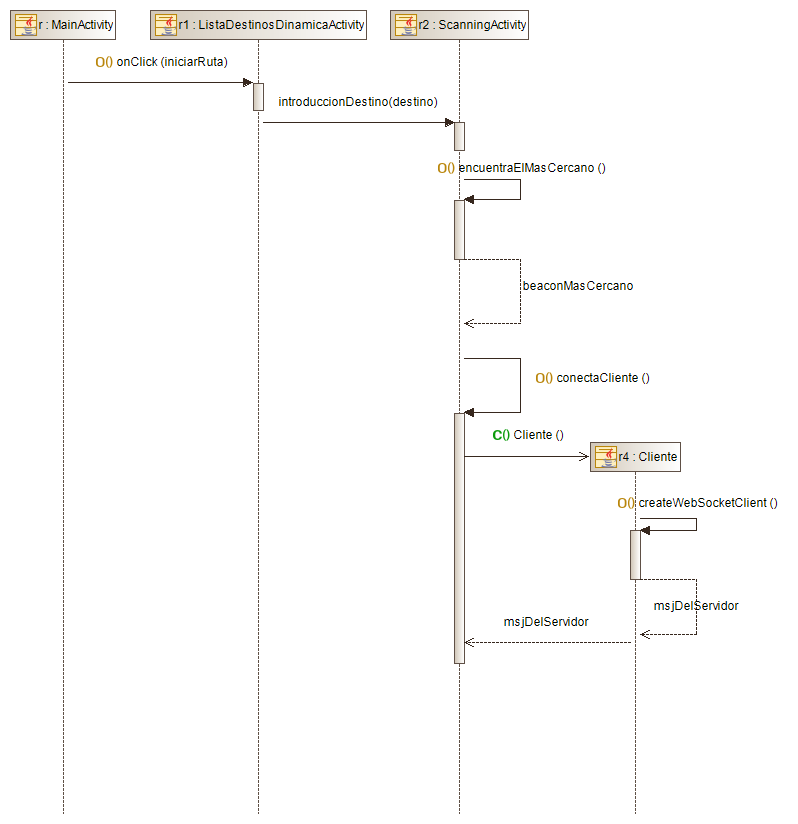
\includegraphics[width=0.8\textwidth]{Imagenes/Capitulo4/diagramasUML/clienteHastaSeguimientoRuta}
		\caption{Diagrama de secuencia que comprende la interacción con el usuario, la resolución del posicionamiento y la conexión con el servidor en el cliente.}
		\label{fig:diag_clientePrimeraParte}
	\end{figure}
		
	\item \textit{Conexión con el servidor}: El código correspondiente a esta funcionalidad se recoge en la clase \textit{Cliente}. Cuando se llama a esta clase se pasan como parámetros el \textit{beacon} más cercano y el destino al que quiere ir el usuario. Con esta información se genera un mensaje del tipo \textit{IDdelBeaconOrigen$|$destino} que se manda al servidor por medio de un \textit{webSocket}. Cuando el servidor genera la ruta manda al cliente un mensaje con toda la información referente a la ruta (ver Sección \ref{sub:func_servidor}). Este mensaje se recibe y desglosa en la lista de \textit{beacons} de la ruta, las instrucciones, la información sobre los giros y la información adicional de los cuadrantes de la ruta. Cuando tiene toda la información avisa a la aplicación (que ha quedado esperando la llegada de este mensaje) y la ejecución continua de nuevo en \textit{ScanningActivity}, donde se guarda la información de la ruta en vectores que se irán recorriendo según avance el usuario. Si no se consigue conectar con el servidor la aplicación genera un mensaje especial que se gestiona en \textit{ScanningActivity} para que la aplicación no quede en espera infinita y acabe bloqueando el dispositivo. En la Figura \ref{fig:diag_clientePrimeraParte} puede verse el diagrama de secuencia que describe las funcionalidades detalladas hasta este momento (interacción con el usuario, posicionamiento y conexión con el servidor).


	\begin{figure}[t]
		\centering
		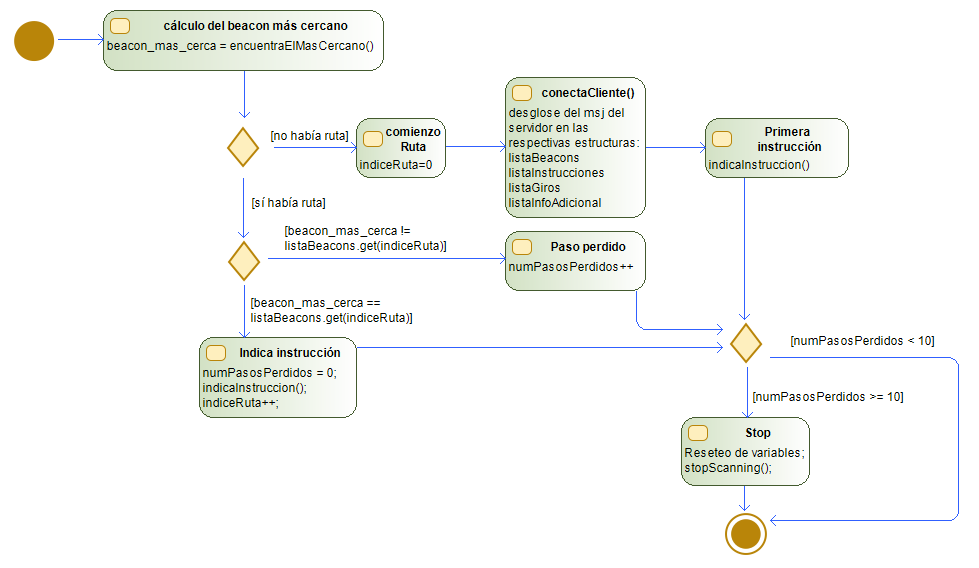
\includegraphics[width=1\textwidth]{Imagenes/Capitulo4/diagramasUML/onEddystonesUpdated}
		\caption{Diagrama de actividad simplificado para la función \textit{onEddystonesUpdated}.}
		\label{fig:diag_clienteSeguimientoRuta}
	\end{figure}

	\item \textit{Seguimiento de la ruta}: Una vez que la conexión con el servidor ha tenido éxito y tenemos toda la información de la ruta almacenada en los vectores correspondientes se comienza guiar al usuario. Para ello se inicia el índice \textit{indiceRuta} a cero y se da al usuario la primera instrucción. Este índice indica en qué punto de la ruta estamos, y cada vez que cambiamos de cuadrante se va incrementando en uno, siempre que estemos siguiendo la ruta. Una vez que el usuario ha recibido la primera instrucción, se va llamando a la función \textit{onEddystonesUpdated} cada dos segundos (parámetro configurable) a fin de saber en qué momento el usuario tiene como \textit{beacon} más cercano el siguiente \textit{beacon} de la ruta. Imaginemos, por ejemplo, que los dos primeros cuadrantes de la ruta fueran el $0$ y el $1$. Cuando se inicia la ruta y el usuario recibe la primera instrucción, la función \textit{onEddystonesUpdated} se dará cuenta de en qué momento el usuario tiene el \textit{beacon1} como más cercano y le dará la siguiente instrucción. Esto mismo ocurre con el resto de \textit{beacons} de la ruta, hasta llegar al final. Si la funcionalidad \textit{Instrucciones detalladas} está activada, se va proporcionando al usuario la información adicional correspondiente a su posición inmediatamente después de la instrucción que debe ejecutar.
	
	Durante la ruta el usuario percibe no solo información oral sobre las instrucciones o la información adicional de los cuadrantes (si tiene la funcionalidad \textit{Instrucciones detalladas} activada), sino también percibe en el dispositivo sonidos y vibraciones. En el caso de que el usuario complete una instrucción, es decir, llegue al siguiente \textit{beacon} de la ruta, la aplicación emite un sonido \textit{check} para hacerle saber que ha completado esa parte. Además, si la instrucción siguiente es un giro, el dispositivo vibra, durante un segundo, si es un giro a la izquierda, y dos vibraciones de medio segundo, si es un giro a la derecha, para notificar el cambio de dirección. Así mismo, cuando el usuario ha llegado al final de la ruta, el dispositivo emite tres vibraciones cortas avisando de que se ha llegado al destino. Esto provoca en el usuario una sensación de control y seguridad, pues puede comprobar en tiempo real que va en el camino correcto y permite que el usuario tenga menos probabilidades de perderse, pues las notificaciones del cambio de sentido están reforzadas.
	
	Se espera que el usuario pueda llegar al destino con la guía que proporciona la aplicación. Sin embargo, también se ha contemplado el hecho de que el usuario se pierda y salga de la ruta. Este caso se detecta cuando se pasa por la función \textit{onEddystonesUpdated} un número determinado de veces\footnote{Este es un parámetro configurable desde el archivo \textit{listasStringApp.xml}. Es el primer elemento del string-array \textit{variables\_ruta}, el segundo corresponde a la variable umbral para \textit{numPasosPerdidos} en caso de que el usuario no detecte ningún \textit{beacon}. Debido a que no se han podido realizar pruebas físicas en la Facultad por la situación sanitaria debida al COVID-19, ajustarlo a lo que podría haber sido una situación real no ha sido posible.}(ver \textit{numPasosPerdidos} en la Figura \ref{fig:diag_clienteSeguimientoRuta}) pero en ninguna de ellas obtenemos que el \textit{beacon} más cercano es el siguiente \textit{beacon} (o un \textit{beacon} más avanzado\footnote{Podría ocurrir que, en un pasillo, por ejemplo, el usuario haya pasado por el siguiente \textit{beacon} pero la aplicación no lo haya detectado. En ese caso el usuario habría avanzado un cuadrante sin notificar a la aplicación, pero como no se ha salido de la ruta se continúa sin notificar al usuario.}) de la ruta. Si esto ocurre, se considera que el usuario se ha salido de la misma. En este caso, cesa el escaneo de los \textit{beacons} y se notifica al usuario que no se encuentra en el camino correcto y que tras pulsar \textit{Iniciar ruta} de nuevo, la aplicación lo redirigirá al destino al que quería ir. En términos de implementación, se vuelve a resolver el problema del posicionamiento, conectar con el servidor e iniciar de nuevo la ruta correspondiente. También se ha contemplado el caso de que el dispositivo no detecte ningún \textit{beacon}. El procedimiento que se sigue es similar al detallado anteriormente, cuando la variable \textit{numPasosPerdidos} llega aun umbral configurable se avisa al usuario de que se encuentra fuera del rango de la aplicación.
	
\end{itemize}


\section{Adaptación para la reutilización de la aplicación sobre otro edificio}
\label{sec:adaptacion}

A lo largo de este capítulo se ha visto la implementación orientada a la Facultad de Informática de la UCM. Sin embargo, no se ha podido realizar un estudio exhaustivo del funcionamiento de la aplicación en esta ubicación debido al estado sanitario de emergencia declarado en marzo de este año 2020 y su posterior prolongación hasta final de curso. Es por ello que se ha tratado de hacer la aplicación lo más genérica posible. De esta manera, si se quisiera utilizar la tecnología \textit{Bluetooth} para mapear otro espacio, nuestro trabajo puede ser reutilizado haciendo una cantidad mínima de cambios. Tanto el código del servidor como el del cliente se han implementado de tal manera que la información relativa al edificio sobre el que se despliega quede reducida a la información contenida en archivos adicionales externos que no forman parte del código. Sin embargo, son algunas las consideraciones que hay que tener en cuenta antes de comenzar con el mapeo de un nuevo espacio. 



\subsection{Cambios en el servidor}
\label{sub:cambiosServidor}

Como se puso de manifiesto en la Sección \ref{sec:servidor}, la información sobre la estructura del edificio que emplea el servidor para el cálculo de la ruta está contenida en los archivos XML y json correspondientes (ver Sección \ref{sec:mapeo}). Gracias a los archivos XML, el servidor conoce los cuadrantes que hay en un piso y, por tanto, sabe identificar cuándo hay que hacer un cambio de planta. Además, conoce la dirección en la que se mueve el usuario ya que sabe la dirección de conexión de los cuadrantes. Así mismo, permite indicar al usuario hacia qué dirección se encuentra su destino en función del camino que haya seguido para llegar a él. De esta manera, el código que genera la ruta es totalmente independiente del edificio. Tan solo se espera que el cambio de planta se haga por medio de un ascensor, lo que parece de esperar cuando se mapean lugares como una facultad o un museo, puesto que las escaleras resultan, en general, complicadas para personas con discapacidad visual y los ascensores suelen estar adaptados mediante botones en braille. De esta manera, para adaptar el servidor a un nuevo espacio tan solo es necesaria la sustitución de estos archivos por los correspondientes al nuevo edificio que se desea mapear. A continuación veremos los aspectos imprescindibles para la realización del nuevo mapeo:


\begin{enumerate}
	\item \textit{Conocer las características del edificio y las necesidades del cliente:} Es importante que antes de plantear el diseño del mapeo del edificio y comenzar a esbozar una estructura de cuadrantes, conozcamos de antemano cómo es el espacio a mapear y qué es lo que se quiere mapear. Ambas cuestiones determinarán la realización del mapeo, pues de ello dependen la forma de los cuadrantes y la ubicación de los \textit{beacons}. 
	
	\item \textit{Trazado de los cuadrantes:} La forma del edificio (intersecciones, puertas, pasillos, ascensores,...) darán forma a los cuadrantes en los que se divide cada una de las plantas del edificio. Hay que tener en cuenta que los cuadrantes deben tener un identificador de tipo entero único (ver \textit{idc} en la Sección \ref{sub:mapeo_xml}) y que estos identificadores deben comenzar en $0$ y continuar la numeración de uno en uno, comenzando por la planta baja del edificio\footnote{De esta manera permitimos que el cuadrante $X$ ocupe la posición $X$ del array de cuadrantes, reduciendo el coste computacional considerablemente. Además, la planta $0$ corresponde con la posición $0$ del array de plantas, la $1$ con la $1$, etc. Si se quisiera incluir un sótano, por ejemplo, este debería tener como identificador de planta $Z = 0$ y el resto de plantas continuar la numeración de uno en uno.}. A la hora de dibujar la estructura de cuadrantes se debe remarcar que cada cuadrante ha de contener exactamente un \textit{beacon} que facilite el posicionamiento del usuario en un punto clave o de decisión, y que todos aquellos cuadrantes carentes de puntos de decisión y, por lo tanto, carentes de \textit{beacons} son cuadrantes inservibles que deben juntarse con otros que sí contengan un punto de decisión.
	
	Una de las características más importantes que han de tener los cuadrantes en los que dividamos nuestro espacio, además de lo ya mencionado sobre los puntos de decisión y las balizas, es que han de confluir con un cuadrante como máximo por cada punto cardinal (norte, sur, este y oeste) ya que más tarde en el archivo XML se almacenará la información de los cuadrantes con los que cada uno está conectado por el norte, sur, este y oeste, y en cada uno de ellos no puede guardarse más de un identificador.
	
	\item \textit{Información de los cuadrantes:} Además de contener las conexiones de los cuadrantes, los archivos XML guardan información relevante para el desarrollo de la ruta como son los metros que ocupa cada cuadrante (que proporcionan al usuario conocimiento de la distancia que tiene que recorrer hasta realizar otra acción), la información asociada a cada uno de ellos o los pesos de la matriz de adyacencia (que son claves para el algoritmo de generación de la ruta (ver Sección \ref{sub:rutaOptima})). Esto último es fundamental, pues se puede ajustar el recorrido de una ruta en caso de que sea necesario por diversas razones: cuestiones de adaptabilidad, reformas de una parte del edificio o aglomeración de gente en una determinada zona del mismo, por ejemplo. Cabe destacar que los cambios no tienen por qué ser estáticos, basta con reiniciar el servidor con los nuevos XML para que los usuarios dispongan de la información actualizada. 
	
	Así mismo, se debe establecer correctamente el lado del cuadrante en el que se encuentra el punto de interés del mismo (norte, sur, este u oeste), pues de ello dependen las instrucciones que indican al usuario dónde se encuentra el destino o las instrucciones que se dan al usuario tras el cambio de planta, en la zona de los ascensores.
	
	\item \textit{Estructuración de los archivos:} Una vez mapeado el edificio, el siguiente paso ha de ser estructurar la información en tres archivos XML que contengan los mismos campos descritos en la Sección \ref{sub:mapeo_xml}: uno de ellos que haga referencia al esqueleto del edificio y los otros dos que plasmen la información de cada una de las plantas.
	
\end{enumerate}

De esta manera, si se quisiera utilizar el código del servidor para otro edificio con los mismos requisitos que la Facultad de Informática de la UCM bastaría con sustituir los archivos correspondientes al edificio, permitiendo así que no se requieran conocimientos específicos de programación para adaptar el código y facilitando su reutilización.


\subsection{Cambios en el cliente}
\label{sub:cambiosCliente}

El cliente es la parte menos dependiente del edificio, puesto que apenas contiene información del mismo. En las Secciones \ref{sub:diseño} y \ref{sub:func_cliente}, revisamos el diseño de la interfaz de la aplicación Blind Bit y su funcionamiento, respectivamente. En cuanto a la interfaz se refiere, es sencillo darse cuenta de que la parte dependiente del edificio corresponde a la pantalla de destinos. Sin embargo, esta está implementada de manera dinámica. Es decir, los nombres de los botones, así como la lista de destinos con la etiqueta correspondiente a los destinos tal y como aparecen en el archivo \textit{destinos.json} del servidor\footnote{Los destinos en la interfaz pueden aparecer con tildes, mayúsculas y otros caracteres especiales que puede no ser posible añadir en el archivo \textit{destinos.json}. Es por ello que se guardan los destinos en dos estructuras, una para la interfaz y otra para la conexión con el servidor.} se guardan en un archivo XML. El archivo donde se guardan estos y otros strings correspondientes a la aplicación, tales como el texto de las instrucciones\footnote{En las instrucciones se incluye también una lista de destinos simplificada, que deberá ser modificada en consonancia con la lista de destinos de la interfaz.} o la uri del servidor, es \textit{listasStringsApp.xml}. Las estructuras referentes a la lista de destinos son \textit{destinos\_array} y \textit{destinosdinamicos\_array}. Mientras que en la primera basta con introducir cada destino en un \textit{<item>}, en la segunda hay que indicar si ese destino tiene un segundo nivel. Por ejemplo, en el caso de la Facultad de Informática tenemos un botón aulas, que no corresponde con un destino sino con el acceso a un segundo nivel donde se muestran las aulas destino disponibles. La estructura que debe seguirse es la siguiente: 

\lstinputlisting[language=XML]{Imagenes/Capitulo4/destinos_array.xml} 

\lstinputlisting[language=XML]{Imagenes/Capitulo4/destinosdinamicos_array.xml}

Donde un ``no'' tras la barra indica que no hay un segundo nivel y cualquier otra cadena de strings se entiende como los destinos correspondientes a ese nivel, separados por comas. Este constituye el único cambio necesario para adaptar el cliente a un nuevo espacio, ya que el código no presenta ninguna dependencia al mismo.



%\section{Adaptación para la reutilización de la aplicación sobre otro edificio}
%
%A lo largo de este capítulo se ha visto la implementación orientada a la Facultad de Informática de la UCM. Sin embargo, no se ha podido realizar un estudio exhaustivo del funcionamiento de la aplicación en esta ubicación debido al estado sanitario de emergencia declarado en febrero de este año 2020 y, su posterior prolongación, hasta final de curso. Así las cosas, se ha tratado de hacer la aplicación lo más genérica posible, de tal manera que, si se quisiera utilizar la tecnología \textit{Bluetooth} para mapear otro espacio, nuestro trabajo pueda ser reutilizado haciendo una cantidad mínima de cambios. A continuación veremos los aspectos que deberían ser modificados.
%
%\subsection{Cambios en el servidor}
%
%El código del servidor se basa, principalmente, en la información del edificio que proporcionan los archivos xml que se vieron en la Sección \ref{sub:mapeo_xml} y el archivo \textit{destinos.json} que se trató en la Sección \ref{sub:func_servidor}. Todos estos archivos deberían ser sustituidos por los correspondientes al nuevo edificio que se desea mapear. Prestando especial atención a los pesos que se colocan en las distintas conexiones de los cuadrantes, pues son claves para el algoritmo de generación de la ruta (ver Sección \ref{sub:rutaOptima}). Así mismo, se debe establecer correctamente el lado del cuadrante en el que se encuentra el punto de interés del mismo (norte, sur, este u oeste), pues de ello dependen las instrucciones que indican al usuario dónde se encuentra el destino o las instrucciones que se dan al usuario tras el cambio de planta, en la zona de los ascensores. De esta manera, si se quisiera utilizar el código del servidor para otro edificio con los mismos requisitos que la Facultad bastaría con sustituir los archivos xml correspondientes al edificio, permitiendo así que no se requieran conocimientos específicos de programación para adaptar el código y facilitando su reutilización.
%
%A pesar de que el código está pensado e implementado para dar servicio a un edificio de características similares a la Facultad de Informática de la UCM también se ha pensado en posibles variantes que podrían surgir a la hora de adaptar el código a otro espacio. A continuación se plantean algunos casos y la solución propuesta: 
%
%\begin{itemize}
%	\item En el caso de la Facultad de Informática hemos establecido que cada cuadrante tiene un único punto de interés. Por ejemplo, los cuadrantes de los pasillos tienen un aula como punto de interés, pero podría ocurrir que en otra facultad hubiera aulas a ambos lados del pasillo y fuera, por tanto, necesario que un cuadrante tuviera más de un punto de interés. Esto se resolvería de manera sencilla adaptando la estructura del cuadrante en los archivos xml: incluyendo una etiqueta que estableciera la ubicación de cada punto de interés y adecuando en el código la lectura del mismo. En el archivo \textit{destinos.json} se incluiría una nueva entrada para el destino, de tal manera que tendríamos dos entradas con el mismo cuadrante (esto no supone un problema pues la clave de la tabla hash donde se almacena la información es el nombre del destino y no el cuadrante). Una vez modificados estos archivos bastaría con indicar a la función \textit{genera} cuál es la ubicación del destino dentro de su cuadrante para que indique al usuario la posición del destino correctamente al finalizar la ruta.
%	
%	\item Otra situación que nos podemos encontrar es aquella en la que la estructura del edificio y los puntos que se quieran mapear se encuentren a una distancia próxima, obligando a que el tamaño de los cuadrantes se vea reducido. En este caso, dar instrucciones al usuario cada cuadrante puede resultar molesto, puesto que se darían instrucciones con demasiada frecuencia. Es por ello que se incluye una variable contador en la función \textit{generar} que permite establecer el número de cuadrantes que queremos ``saltar'' antes de dar una nueva instrucción\footnote{En el propio código se han incluido en comentarios los cambios necesarios para la implementación de esta funcionaliadad.}, siempre que la dirección del usuario se mantenga estable. Es decir, no haya que hacer un giro, pues en ese caso debemos advertir al usuario.
%\end{itemize}


%Todos los cambios mencionados, a excepción de los archivos que no forman parte del código, constituyen cambios necesarios para adaptar el edificio a personas con discapacidad visual, puesto que, si la aplicación no estuviera diseñada para ellos no habría necesidad de dar indicaciones tan detalladas.


%\subsection{Cambios en el cliente}

%El cliente es la parte menos dependiente del edificio, puesto que en ningún momento contiene información del mismo, a excepción de la lista de destinos que se incluye tanto en la interfaz como en el archivo \textit{listasStringsApp.xml}. En este archivo se encuentran los destinos con el mismo nombre que el servidor los representa en el archivo \textit{destinos.json}, lo que permite que antes de conectar con el servidor podamos comprobar que el destino es correcto. También habría que modificar esta lista de destinos en las instrucciones de uso de la aplicación para que el usuario pueda acceder a ella sin necesidad de tener que simular el inicio de una ruta.




\chapter{Evaluación}
\label{cap:evaluacion}

En este capítulo se describe el proceso de evaluación de la aplicación que se ha llevado a cabo. Como ya se puso de manifiesto en el Plan de trabajo (ver Sección \ref{sec:planTrabajo}), la idea inicial era la de realizar una evaluación con usuarios finales y, preferiblemente, en la Facultad de Informática de la UCM, pues ese espacio es nuestro caso de estudio inicial. Debido a la crisis sanitaria y el estado de emergencia declarado en marzo de 2020 a causa de la COVID-19, no ha sido posible la ejecución de dicha evaluación. Sin embargo, conseguimos sobreponernos a este contratiempo y poner de manifiesto la flexibilidad de la aplicación mapeando otro edificio y realizando diversas pruebas sobre este. Este edificio no pudo ser otro que una vivienda. Cabe destacar que este no es el escenario ideal sobre el que se desplegaría una aplicación como Blind Bit, pues el espacio queda considerablemente reducido en comparación con el de una facultad o museo, por ejemplo. A pesar de ello, permite probar el comportamiento de la aplicación en situaciones donde cierta aglomeración de \textit{beacons} es necesaria y poner a prueba el mapeo de un edifico con características distintas al ya planteado en la Sección \ref{sec:mapeo}. En las secciones que siguen se detalla cómo se ha llevado a cabo la adaptación tanto del plan de evaluación como el despliegue de la aplicación en otro edificio.

En la Sección \ref{sec:adaptacionApp} se describen los pasos a seguir, tanto en el servidor (Sección \ref{sub:cambiosServidor_vivienda}) como en el cliente (Sección \ref{sub:cambiosCliente_vivienda}) para poder adaptar la aplicación al nuevo espacio. Por su parte, la Sección \ref{sec:objetivosEval} detalla los objetivos de la evaluación. Las pruebas que se llevaron a cabo a fin de valorar el cumplimiento de estos objetivos se exponen en la Sección \ref{sec:realizYresult} y las conclusiones finales de la evaluación pueden verse en la última sección (Sección \ref{sec:conclusionesEval}).


\section{Adaptación de la aplicación al nuevo edificio}
\label{sec:adaptacionApp}

En esta sección detallaremos los cambios que se han realizado para poder desplegar Blind Bit sobre la vivienda. Veremos tanto los cambios referentes al servidor (Sección \ref{sub:cambiosServidor_vivienda}) como al cliente (Sección \ref{sub:cambiosCliente_vivienda}). Hay que tener en cuenta que ninguno de estos cambios implica la modificación del código de la aplicación, pues esta se ha implementado de manera genérica para permitir su reutilización en nuevos espacios como el que se expone a continuación.

\subsection{Cambios en el servidor}
\label{sub:cambiosServidor_vivienda}

En la Sección \ref{sub:cambiosServidor} se exponen las claves para realizar el mapeo de un nuevo edificio. A continuación veremos cómo se han aplicado estas para el mapeo de la vivienda.


A la hora de enfrentarnos al mapeo de este nuevo edificio hemos seguido la estructura definida en la Sección \ref{sec:mapeo} del Capítulo \ref{cap:descripcionTrabajo} y la hemos representado como archivos XML siguiendo el mismo formato descrito en la Sección \ref{sub:mapeo_xml} del mismo capítulo.

Para ello, lo primero ha sido dividir el edificio en cada una de sus plantas y finalmente dividir estas en cuadrantes únicos. Para realizar esta tarea hay que tener en consideración que tal y como ya habíamos concluido, cada cuadrante ha de contener exactamente un \textit{beacon} que facilite el posicionamiento del usuario en un punto clave o de decisión y que todos aquellos cuadrantes carentes de puntos de decisión y por lo tanto carentes de \textit{beacons} son cuadrantes inservibles que deben juntarse con otros que si contengan un punto de decisión. De esta manera en la Figura \ref{fig:mapeoCasa} podemos ver en rojo la división hecha de cada una de las plantas en sus cuadrantes, cuyos identificadores son los números que aparecen sobre ellos y en los que la ubicación de los \textit{beacons} está representada con un círculo amarillo. Una de las características más importantes que han de tener los cuadrantes en los que dividamos nuestro espacio, además de lo ya mencionado sobre los puntos de decisión y las balizas, es que han de confluir con un cuadrante como máximo por cada punto cardinal (norte, sur, este y oeste) ya que más tarde en el XML se almacenará la información de los cuadrantes con los que cada uno está conectado por el norte, sur, este y oeste, y en cada uno de ellos no puede guardarse más de un identificador.

A diferencia del trabajo realizado en la Facultad de Informática, en este caso sí hemos mapeado las distintas estancias, esto se debe a la naturaleza tan distinta de este edificio que al ser una vivienda particular presenta dimensiones mucho inferiores y por lo tanto, hemos de decidido mapear todo el espacio para añadir complejidad a la guía y que esta no se limite a ir de puerta a puerta.

En la Figura \ref{fig:mapeoCasaPBaja} vemos como hemos dividido la planta baja de la vivienda en 11 cuadrantes, siendo este último el que se corresponde con las escaleras que unen esta planta con el cuadrante 12 de la planta superior. El mapeo de la primera planta se encuentra en la Figura \ref{fig:mapeoCasaPAlta} que como vemos tiene la misma estructura que la planta inferior a excepción de la superficie que se corresponde con los cuadrantes $0$, $1$ y $10$ que desaparecen. Solo hemos incluido dos cuadrantes ya que la división es completamente análoga.

Una vez mapeado el edificio el siguiente paso ha de ser estructurar la información en tres archivos XML que contengan los mismos campos descritos en la Sección \ref{sub:mapeo_xml}. Uno de ellos que haga referencia al esqueleto del edificio y los otros dos que plasmen la información de cada una de las plantas. %En el Apéndice X podemos ver estos archivos XML.



\subsection{Cambios en el cliente}
\label{sub:cambiosCliente_vivienda}

En las Secciones \ref{sub:diseño} y \ref{sub:func_cliente}, revisamos el diseño de la interfaz de la aplicación Blind Bit y su funcionamiento, respectivamente. En cuanto a la interfaz se refiere, es sencillo darse cuenta de que la parte dependiente del edificio corresponde a la pantalla de destinos. Sin embargo, esta está implementada de manera dinámica. Es decir, los nombres de los botones, así como la lista de destinos con la etiqueta correspondiente a los destinos tal y como aparecen en el archivo \textit{destinos.json} del servidor\footnote{Los destinos en la interfaz pueden aparecer con tildes, mayúsculas y otros caracteres especiales que puede no ser posible añadir en el archivo \textit{destinos.json}. Es por ello que se guardan los destinos en dos estructuras, una para la interfaz y otra para la conexión con el servidor.} se guardan en un archivo xml. El archivo donde se guardan estos y otros strings correspondientes a la aplicación, tales como el texto de las instrucciones o la uri del servidor es \textit{listasStringsApp.xml}. Las estructuras referentes a la lista de destinos son \textit{destinos\_array} y \textit{destinosdinamicos\_array}. Mientras que en la primera basta con introducir cada destino en un \textit{<item>}, en la segunda hay que indicar si ese destino tiene un segundo nivel. Por ejemplo, en el caso de la Facultad de Informática tenemos un botón aulas, que no corresponde con un destino sino con el acceso a un segundo nivel donde se muestran las aulas destino disponibles. La estructura que debe seguirse es la siguiente: 


%\lstinputlisting[language=XML]{Imagenes/Evaluacion/destinos_array.xml} 

%\lstinputlisting[language=XML]{Imagenes/Evaluacion/destinosdinamicos_array.xml}

Donde un ``no'' tras la barra indica que no hay un segundo nivel y cualquier otra cadena de strings se entiende como los destinos correspondientes a ese nivel, separados por comas. Este constituye el único cambio necesario para adaptar el cliente a un nuevo espacio.

\section{Objetivos de la evaluación}
\label{sec:objetivosEval}

Debido a la imposibilidad de realizar una evaluación con usuarios. Nos vimos obligadas a reestructurar el \textit{modus operandi} de la evaluación de la aplicación. Concretamente, los objetivos cambiaron, centrándose en el funcionamiento de la misma y dando menos peso a la usabilidad, en la que los usuarios finales tienen un papel decisivo. De esta manera, se decidió establecer cuatro objetivos claros que presentamos a continuación:

\begin{enumerate}
	
	\item \textit{Resolución del problema del posicionamiento:} Una de las funcionalidades principales de la aplicación es, sin duda, la correcta ubicación del usuario. Para ello es necesario que el \textit{beacon} más cercano al usuario sea detectado como el más cercano por la aplicación (ver Sección \ref{sub:func_cliente}). De esta tarea depende no solo el inicio de la ruta sino el seguimiento de toda ella, pues en todo momento debemos conocer el cuadrante donde se encuentra el usuario para que la aplicación pueda responder en consecuencia. Una mala ubicación del usuario podría provocar que el usuario se pierda debido a indicaciones que no corresponden con su posición o, en casos más graves, el tropiezo o golpeo del usuario con un obstáculo del que no ha sido advertido.
	
	Cabe destacar que en el posicionamiento influye no solo la correcta implementación del código, sino también la ubicación de los \textit{beacons}, que debe adaptarse a las necesidades específicas de cada edificio. 
	
	\item \textit{Generación de instrucciones correctas:} Teniendo en cuenta la ubicación del usuario y el camino que ha seguido, es primordial que la aplicación sea capaz de generar instrucciones correctas. Tanto los giros como la señalización de puntos de interés como los ascensores o el destino debe corresponderse con la ubicación real de estos, tal y como se establece en los archivos xml (ver Sección \ref{sub:mapeo_xml}).
	
	\item \textit{Precisión de las instrucciones:} Además de que las instrucciones sean correctas, hay que evaluar que el usuario las recibe en el momento adecuado. Esto está claramente relacionado con el posicionamiento, pues el momento de indicación de la ruta se basa en cuándo el usuario llega a un determinado cuadrante. Sin embargo, se debe prestar especial atención a las posibles variaciones que pueden darse (una instrucción puede darse con cierta antelación o, por el contrario, una vez pasado el punto óptimo) y evaluar si esa flexibilidad es asumible para el usuario.
	
	\item \textit{Ejecución correcta en caso de usuario perdido:} Este es un punto importante, pues no debemos asumir que el usuario va a seguir siempre la ruta, puede ocurrir que por diversos motivos (una distracción, un obstáculo o el propio fallo de la aplicación) el usuario se desvíe de la ruta. En ese caso no solo se debe identificar el problema sino también saber reconducir al usuario al destino deseado. 
		
\end{enumerate}


\section{Realización y resultados de la evaluación}
\label{sec:realizYresult}

La realización de la evaluación no pudo darse en el edificio objetivo de nuestro estudio (la Facultad de Informática de la UCM) debido a la imposibilidad de acceder a él. Sin embargo, conseguimos sobreponernos a este contratiempo y poner de manifiesto la flexibilidad de la aplicación mapeando otro edificio y realizando diversas pruebas sobre este. Este edificio no pudo ser otro que una vivienda. Cabe destacar que este no es el escenario ideal sobre el que se desplegaría una aplicación como Blind Bit, pues el espacio queda considerablemente reducido en comparación con el de una facultad o museo, por ejemplo. A pesar de ello, permite probar el comportamiento de la aplicación en situaciones donde cierta aglomeración de \textit{beacons} es necesaria y poner a prueba el mapeo de un edifico con características distintas al ya planteado en la Sección \ref{sec:mapeo}.

\subsection{Mapeo del nuevo espacio}

Como ya se avanzaba en la introducción, el edificio sobre el que se basa la evaluación es una vivienda. En la Figura \ref{fig:mapeoCasa} vemos el resultado del mapeo, donde el número de cuadrante está recuadrado en negro, la posición de los beacons en amarillo y los cuadrantes vienen delimitados por las líneas rojas y las paredes de la vivienda. Como muestra la Figura \ref{fig:mapeoCasaPAlta}, el mapeo de la planta alta se ha reducido a dos cuadrantes, pues son suficientes para \textit{testear} las rutas que incluyen un cambio de planta ya que la estructura es análoga a la de la planta baja.


\begin{figure}[t!]
	\centering
	
	\subfloat[Mapeo de la planta baja de la vivienda]{
		\label{fig:mapeoCasaPBaja}
		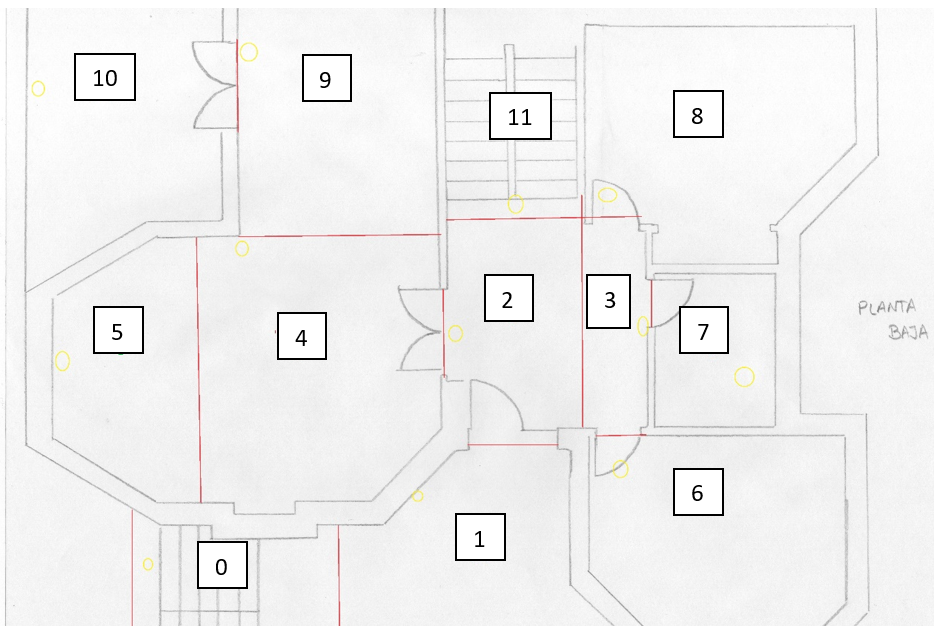
\includegraphics[width=0.8\textwidth]{Imagenes/Evaluacion/planoCasaPBaja}}
	
	\subfloat[Mapeo de la planta alta de la vivienda]{
		\label{fig:mapeoCasaPAlta}
		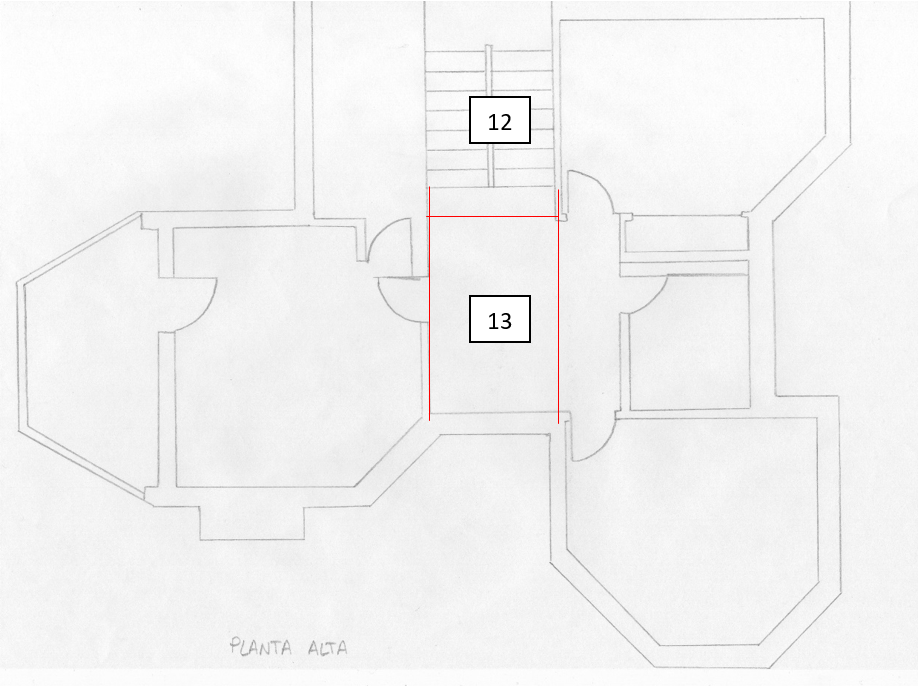
\includegraphics[width=0.8\textwidth]{Imagenes/Evaluacion/planoCasaPAlta}}\\
	
	\caption{Mapeo de la vivienda}
	\label{fig:mapeoCasa}
\end{figure}

A continuación se describen las pruebas realizadas y se analizan los resultados obtenidos.

\subsection{Seguimiento de la ruta}
En esta sección se detallan las pruebas realizadas asumiendo que el usuario no va a salir de la ruta. Sin embargo, algunas de ellas están diseñadas para reproducir situaciones extremas como la pérdida de un \textit{beacon} o rutas potencialmente complicadas.


\subsubsection{Ruta del cuadrante $0$ al cuadrante $10$}
\label{subsub:0al10}
La primera ruta de la evaluación consiste en realizar la ruta desde el cuadrante $0$ hasta el cuadrante $10$ sin salir de la ruta. En esta se debe prestar especialmente atención a las instrucciones de giro, pues son constantes durante toda la ruta. Además, no debemos olvidar que la aplicación emite distintas vibraciones en función de la dirección de giro. Estas vibraciones deben quedar lo suficientemente claras para el usuario. 

Este recorrido se realizó varias veces a fin de encontrar irregularidades en la ruta. A continuación se detallan las conclusiones obtenidas:

\begin{itemize}
	\item Las instrucciones generadas por la aplicación son correctas y, en la mayor parte de los casos, se indican al usuario en el momento adecuado.
	
	\item Las vibraciones asociadas a los giros y a la llegada del destino son lo suficientemente distintas para que el usuario pueda distinguirlas.
	
	\item En dos ocasiones las instrucciones correspondientes a los cuadrantes $1$ y $2$ se dieron demasiado pronto. Esto puede deberse a que el \textit{beacon} del cuadrante $1$ está situado en el exterior y que, una vez que se avanza hacia la puerta que separa los cuadrantes $1$ y $2$, la distancia que hay entre ellos es reducida.
	
	\item En una de las ocasiones el \textit{beacon} asociado al cuadrante $4$ no fue detectado por la aplicación, provocando la pérdida de esa instrucción (en las pruebas siguientes se detalla el comportamiento de la aplicación en este caso. Ver Secciones \ref{subsub:0al10sin4} y \ref{sub:usuarioPerdido}).
	
	\item Una vez se ha llegado al destino, la posición del mismo se indica correctamente en función de la dirección desde la que proviene del usuario.
	
\end{itemize}

\subsubsection{Ruta del cuadrante $1$ al cuadrante $10$}

Este caso es prácticamente idéntico al anterior (Sección \ref{subsub:0al10}), con la única diferencia que se pone a prueba el posicionamiento inicial del usuario. Tras comprobar que las instrucciones en el cuadrante $1$ se daban antes de lo previsto en algunas ocasiones, se decidió empezar la ruta en este cuadrante. De esta manera la aplicación debía detectar el \textit{beacon$1$} como \textit{beacon} más cercano. Se hicieron cinco pruebas y se pudo comprobar que en dos ocasiones este posicionamiento no se realizó de manera correcta. En uno de ellas el \textit{beacon} más cercano detectado por la aplicación fue el $4$ (lo que puede ser provocado porque la separación entre el $4$ y el $1$ es una ventana) y en otra el $2$ (cuya posible explicación  ya fue mencionada en la Sección \ref{subsub:0al10}).

\subsubsection{Ruta del cuadrante $0$ al cuadrante $10$, eliminando el \textit{beacon} del cuadrante $4$}
\label{subsub:0al10sin4}

En este caso se ha vuelto a repetir la ruta del cuadrante $0$ al $10$ con la particularidad de que el \textit{beacon$4$}\footnote{Asumiremos que \textit{beaconX} es el \textit{beacon} asociado al cuadrante X.} fue eliminado de la ruta. Sin embargo, no provocamos la situación de que el usuario se saliera de la ruta (como sería lógico en esta situación, pues la instrucción de giro del cuadrante $4$ se pierde), continuamos por el cuadrante $9$. De esta manera la aplicación no notifica que el usuario se ha perdido, pues sigue en la ruta. A pesar de que la instrucción indicada en el cuadrante $9$ fue la correcta (giro a la izquierda), la aplicación tardó demasiado. Esto se debe a que el umbral de la variable \textit{numPasosPerdidos}, que identifica el momento en el que el usuario puede haberse perdido (ver Sección \ref{sub:func_cliente}), es demasiado elevado para este edificio, donde las distancias entre \textit{beacons} son pequeñas.


\subsubsection{Ruta del cuadrante $1$ al cuadrante $5$, eliminando el \textit{beacon} del cuadrante $2$}
\label{subsub:1al5sin2}

Este caso es interesante, pues, a pesar de que se ha eliminado uno de los \textit{beacons} correspondientes a una intersección, la información de giro del cuadrante $2$ no se pierde. Esto se debe a que, como la aplicación es capaz de avisar de los cambios de dirección con antelación, en el cuadrante $1$ ya se indica al usuario que, tras avanzar unos metros, debe girar a la izquierda. Bien es cierto que se pierde precisión, pues el usuario no percibe la instrucción de giro en el momento en el que debe realizarse, ni la confirmación sonora y vibración asociada a esta. Sin embargo, el hecho de que se den instrucciones por adelantado favorece que el usuario permanezca en la ruta aún cuando alguna instrucción se pierda. 

Particularmente para esta ruta, el giro del cuadrante $2$ es el único que hay que realizar y, debido a esto, es más fácil que el usuario no se pierda. Si, por el contrario, el destino hubiera sido el cuadrante $10$, es probable que el usuario no hubiera llegado a recibir la instrucción de giro a la derecha del cuadrante $4$ tampoco. Esto se debe a que la aplicación necesita un tiempo (llegar a un número de pasos perdidos) para decidir si el usuario se ha perdido. De esta manera, cuando el usuario llega al cuadrante $4$ la aplicación sigue a la espera del cuadrante $2$ (el umbral de \textit{numPasosPerdidos} es demasiado alto. Ver funcionamiento en la Figura \ref{fig:diag_clienteSeguimientoRuta}). Esto implica que el usuario se salga de la ruta. Caso que abordamos en la Sección \ref{sub:usuarioPerdido}.


\subsubsection{Ruta del cuadrante $1$ al cuadrante $13$}

En este caso, lo que se quería evaluar eran las instrucciones referentes al cambio de planta. Como ya se comentó en la Sección \ref{sub:cambiosServidor}, el código asume que los cambios de planta se realizan por medio de ascensores. Esta información se ha ignorado en esta ocasión, pues solo se disponía de escaleras. 

De la ruta desde el cuadrante $1$ al $13$ destacamos un punto importante, que es la anticipación de los ascensores en el cuadrante $2$ gracias a la información adicional generada. Esto avisa al usuario del cambio de planta. Una vez en el cuadrante $11$, la aplicación indica al usuario a qué planta se debe dirigir y en qué dirección se encuentran los ascensores (en este caso, delante del usuario). Una vez en la planta superior, la instrucción del cuadrante 12 continua teniendo en cuenta la nueva orientación del usuario (continúa recto). 

\subsubsection{Ruta del cuadrante $13$ al cuadrante $8$}
\label{subsub:13al8}

La finalidad de esta ruta es, principalmente, comprobar el comportamiento de la aplicación en el \textit{hall} de la planta baja, así como el cambio de planta inverso. 

El problema que surge aquí es que los giros que hay que realizar en la planta baja son bastante tediosos. Por un lado, la ubicación del \textit{beacon$2$} favorece que la instrucción de giro hacia el \textit{beacon$3$} tarde demasiado en llegar. Una vez que se proporciona esta instrucción, el cuadrante $3$ vuelve a hacer girar al usuario hacia el $8$, lo que provoca cierta confusión. De igual manera se probó la ruta inversa, desde el cuadrante $8$ al $13$, y el resultado fue análogo.


\subsubsection{Ruta del cuadrante $9$ al cuadrante $13$}
\label{subsub:9al13}

Como la ruta por el \textit{hall} de la planta baja había resultado tediosa en el caso anterior, se hizo una prueba desde el otro extremo. Esta vez la ubicación del \textit{beacon$2$} favorece el giro del usuario para encontrar el ascensor (escaleras en este caso). De esta manera la ruta resulta mucho más natural y organizada que en el caso anterior.

\subsection{Usuario perdido}
\label{sub:usuarioPerdido}

En esta sección se expone el comportamiento de la aplicación cuando el usuario sale de la ruta, basado en ejemplos de ejecución reales. 

En la Sección \ref{subsub:0al10sin4} vimos un caso en el cual era probable que un usuario se desviara de la ruta, debido a la pérdida de la instrucción de giro asociada al cuadrante $4$. De esta manera el usuario continuaría hasta llegar al cuadrante $5$. Es entonces cuando la aplicación detecta que el usuario se ha salido de la ruta e indica al usuario que debe volver por la dirección en la que venía y le permite iniciar de nuevo la ruta al destino desde su posición actual. Como ya se ha comentado, esta indicación se da con cierto retraso debido a que el valor que debe alcanzar la variable \textit{numPasosPerdidos} es demasiado elevada para este edificio. 

Además, la aplicación está preparada para el caso en el que no se detecte ningún \textit{beacon}. Si no se produjera ninguna detección transcurrido un tiempo (determinado por una variable umbral), la aplicación advierte al usuario de la situación indicándole que debe posicionarse dentro del edificio\footnote{Se asume que si ningún \textit{beacon} es detectado es porque el usuario no se encuentra dentro del edificio o la zona mapeada}. Esta situación se reprodujo avanzando hacia la izquierda del cuadrante $0$ y eliminando los \textit{beacons} más próximos a esa zona para provocar que ninguno de ellos fuera detectado.

A pesar de que no ha sido detallado expresamente durante la realización de las pruebas, hay que mencionar que el resto de funcionalidades como el modo silencio, la repetición de la última instrucción, el modo instrucciones detalladas y la finalización anticipada de la ruta también fueron comprobados, sin destacar ningún comportamiento extraño o inesperado.

\section{Conclusiones de la evaluación}
\label{sec:conclusionesEval}

En las pruebas realizadas y descritas en la Sección \ref{sec:realizYresult} se ha puesto de manifiesto el comportamiento de la aplicación en situaciones normales y extremas. Abordando también aquellos casos en los que el usuario se pierde. En esta sección se exponen los puntos más relevantes obtenidos tras el análisis de las situaciones vistas.


\begin{itemize}
	\item \textit{El código de la aplicación funciona de la manera esperada:} A lo largo de las numerosas rutas de prueba se ha podido comprobar que las instrucciones, vibraciones y sonidos se reproducen e indican al usuario de la manera esperada. No se ha apreciado ningún comportamiento inesperado o erróneo. 
	
	\item \textit{El mapeo del edificio juega un papel primordial:} Como se puede observar en las Secciones \ref{subsub:13al8} y \ref{subsub:9al13} la disposición de los cuadrantes y \textit{beacons} puede facilitar la ruta al usuario en gran medida. Por ello, cuantos menos cuadrantes más sencilla será la ruta. La ubicación de los \textit{beacons} debe ser lo más neutra posible. Es decir, que no favorezca más una ruta que otra.
	
	\item  \textit{Se debe ajustar el umbral de la variable numPasosPerdidos al espacio comprendido entre los beacons:} Han sido varias las ocasiones donde se ha puesto en evidencia que las indicaciones sobre el cambio de ruta debían haberse proporcionado con anterioridad. Para solucionarlo basta con reducir este umbral, teniendo en cuenta que el tiempo que tarda en recorrer un espacio una persona con discapacidad visual suele ser ligeramente mayor.
	
	\item \textit{La generalidad de la aplicación:} Debido a las circunstancias, la evaluación de la aplicación ha sido realizada en un edificio distinto a la Facultad de Informática de la UCM. Gracias a una implementación general, apenas dependiente del espacio donde se despliega, el esfuerzo para poder adaptarla queda reducido a la realización de los archivos xml y json de la Sección \ref{sec:mapeo}.
	
	\item \textit{Ventajas de las instrucciones e información adicional anticipadas:} Como pudimos ver en la Sección \ref{subsub:1al5sin2}, el hecho de que las instrucciones de giro se avisen con un cuadrante de antelación prepara al usuario para el cambio de dirección, favoreciendo que este no se salga de la ruta, y, en caso de que el \textit{beacon} de la intersección no se detecte, facilita que la información de la ruta persista. Lo mismo ocurre con la información adicional, sobre todo en el caso de los ascensores, pues permite al usuario identificar que debe cambiar de planta para llegar a su destino por adelantado.

\end{itemize}



\chapter{Trabajo individual}
\label{cap:trabajoIndiv}

En este capítulo se detalla el trabajo realizado por cada integrante del grupo de trabajo de este proyecto. En la Sección \ref{sec:trabajoBelen} se expone el trabajo realizado por Belén Serrano Antón, mientras que la Sección \ref{sec:trabajoClara} expone el de Clara de Suso Seijas.

\section{Belén}
\label{sec:trabajoBelen}

Antes de decidir el tema sobre el que iba a realizar mi Trabajo de Fin de grado, abordé con Raquel Hervás diferentes posibilidades a finales del curso anterior. Todas ellas tenían un punto en común: la mejora del día a día del usuario final. El resultado de esas investigaciones previas acabaron derivando en el proyecto expuesto a lo largo de este documento, que tiene como finalidad la adaptación del interior de un edificio a personas con discapacidad visual. Ya en septiembre de este curso el equipo de trabajo se cerró con la llegada de Clara.

Ambas comenzamos a estudiar distintos trabajos que se habían hecho en el área de la navegación por interiores y que conforma el Capítulo \ref{cap:estadoDeLaCuestion}. Nos repartimos el trabajo entre las dos, mientras que yo me encargué de la investigación de las aplicaciones \textit{Google Maps} y \textit{BlindSquare}, Clara ultimó el resto. Además, tuvimos la oportunidad de entrevistarnos en el Centro de Tiflotecnología e Innovación de la ONCE gracias a la profesora María Guijarro. Entre Clara y yo recogimos las notas que, posteriormente, darían lugar al Capítulo \ref{cap:once}.

Una vez se habían sentado las bases del trabajo y establecido que la tecnología utilizada iban a ser las balizas Bluetooth, me encargué de salvar la primera barrera tecnológica: poner en funcionamiento los \textit{beacons}. Para ello fue necesaria la revisión de la SDK de \textit{Kontakt}, así como la realización de diversos tutoriales a partir de los cuales ganar soltura con el nuevo entorno de desarrollo, Android Studio. El tiempo invertido en ello me permitió implementar dos aplicaciones sencillas pero funcionales, \textit{miniapp} y \textit{cuadrantes\_v1} (ver Sección \ref{sec:estudioPrecisionBeacons}). Más tarde implementaría \textit{pruebaSonido}, que recoge la lógica necesaria para detectar el \textit{beacon} más cercano. Gracias a ellas se pudo comenzar el estudio de la precisión y el comportamiento de las balizas. Las mediciones expuestas en el Capítulo \ref{cap:descripcionTrabajo} (ver Sección \ref{sub:pruebasCuadrantesv1}) y en el Anexo \ref{Appendix:ResMediciones}, son el resultado de varios días de trabajo en los que se trataron distintas ubicaciones de los \textit{beacons} y se tomaron decisiones sobre la posición en la que se colocarían. Algunas de esas jornadas Clara y yo trabajamos de manera conjunta en la Facultad de Informática de la UCM y, en otras ocasiones, hice yo mediciones en solitario, cuyos resultados compartiría con Clara para su posterior discusión. Tras el estudio de los datos obtenidos se elaboraron de manera conjunta gráficas que permitieran observar el comportamiento de los \textit{beacons} de manera simplificada.

\subsection{Servidor}

Antes de comenzar con el mapeo de la Facultad ambas revisamos el trabajo de \cite{TFGguia}, con la intención de encontrar un modelo de mapeo en el que sustentar el nuestro. Además, revisamos el código del servidor de este mismo trabajo, a partir del cual me encargué de la total adaptación del mismo a nuestro proyecto\footnote{A excepción de los archivos de lectura de XML, que serían modificados por ambas a partir de la nueva información añadida.}. Para ello, en primer lugar tuve que implementar una clase Cliente en Java a través de la cual mandar mensajes al servidor para observar el funcionamiento del código. El resultado de este estudio fue la rápida sustitución del algoritmo que generaba los cuadrantes de la ruta por el algoritmo de \textit{Dijkstra}, debido a que la otra versión no generaba una lista ordenada de cuadrantes, que era lo que se buscaba. Tras ese cambio fueron diversas las pruebas que realicé utilizando los archivos XML de \cite{TFGguia}. Una vez comprobado que el código del servidor funcionaba (al menos técnicamente), Clara se encargó de realizar el mapeo de la Facultad. Mientras tanto, seguí haciendo modificaciones sobre el código del servidor. Entre ellas, numerosos cambios en la función \textit{generar}. Esta función se adaptó a lo que nosotras buscábamos: instrucciones en cada cuadrante, indicación sobre la posición final del destino, adición de información adicional sobre la ruta, etc (ver Sección \ref{sub:genInstruc}). De estos cambios destaca el hecho de que el código encargado de señalizar los giros (ver Sección \ref{sub:instr_giro}) quedó simplificado en gran medida y de que de la función \textit{generar} se eliminaron todas las dependencias del edificio\footnote{Cabe destacar que este proceso fue iterativo y fueron muchas las pruebas realizadas durante el mismo a fin de obtener un código libre de errores (o lo más libre posible).}. Esto último implicó fijar el orden en el que los archivos XML son leídos. Puesto que el código debe ser independiente del número de plantas del edificio, se presupone que el argumento de \textit{Z} (ver Sección \ref{sub:mapeo_xml}) en el XML, que corresponde con el número de planta, es la posición del array en el que se guardan los cuadrantes que pertenecen a una planta. De esta manera, los cuadrantes con $Z = 0$ se guardan en la posición $0$, los de $Z = 1$ en la posición $1$ y así sucesivamente. Esto no ocurría en la primera versión, puesto que comenzamos a mapear la Facultad por la primera planta. Tras darme cuenta de este problema, decidí renombrar todos los cuadrantes mapeados, tanto en los XML como en las referencias de la memoria, comenzando por la planta baja\footnote{Hay que tener en cuenta que el cuadrante \textit{i-ésimo} del array de cuadrantes debe corresponder con el cuadrante con identificador $i$.}, permitiendo así el mapeo de cuantas plantas se quieran. Otra consecuencia de la generalidad de la función \textit{generar} fue la adición de información a los archivos XML. Concretamente añadí los pesos de la matriz de adyacencia, que hasta entonces se modificaban desde el código, y la posición del punto de interés de un cuadrante, que anteriormente se asumía dependiendo del número de este. 

Otro de los grandes cambios del servidor que realicé fue la sustitución de la conexión cliente-servidor, cambiando los \textit{sockets} por \textit{webSockets}. Lo que se buscaba con ello es que el código del servidor pudiera quedar en un servidor externo, de manera que conociendo su \textit{uri}, se pudiera acceder desde cualquier red. Esto suponía un punto fundamental, pues sin ello no se podía probar la aplicación desde la Facultad\footnote{Hasta entonces las pruebas las había realizado sobre la red interna de mi casa.}. Raquel y Gonzalo gestionaron el acceso a un repositorio \textit{Holstein}, desde el cual traté, en numerosas ocasiones, instalar Tomcat y poner en funcionamiento una conexión mediante \textit{webSockets}. Finalmente, tras varias semanas sin encontrar el error y debido a la imposibilidad de acudir a la Facultad\footnote{Debido a la crisis sanitaria por la COVID-19.} por si fuera necesario un reinicio del servidor por la modificación de alguno de sus parámetros de configuración, Gonzalo nos dio acceso a una máquina virtual de la Universidad. Esta vez la instalación de Tomcat\footnote{Los \textit{webSockets} están disponibles a partir de la versión $9$ de Tomcat.} y el posterior despliegue del código del servidor sí tuvo éxito. Una vez se resolvió la parte técnica de esta conexión implementé un nuevo Main para el servidor, el cual recibía la información del cliente por medio de un \textit{webSocket}. A fin de poder realizar pruebas en el servidor sin tener que utilizar mi dispositivo móvil ni los \textit{beacons}, elaboré un archivo \textit{WebSocketClient.html} muy sencillo a través del cual poder mandar mensajes al servidor y leer su respuesta. Esto fue de gran ayuda pues me permitió probar numerosas rutas sin necesidad de simularlas mediante \textit{beacons}. De esta manera cuando realizaba pruebas desde la aplicación sabía de antemano que el código del servidor funcionaba, ayudándome a descartar posibles fallos de este. 

En cuanto a la memoria, me encargué de la redacción de la Sección \ref{sec:servidor}.

\subsection{Cliente}

Respecto al cliente, mi trabajo comenzó con los primeros bocetos de la interfaz, que fueron discutidos y modificados entre Clara y yo, y, posteriormente, con los directores. Yo me encargué de la implementación de la pantalla \textit{Principal} y de una versión anterior de la pantalla \textit{Destinos}, en la cual los botones destino no eran dinámicos, incluyendo la funcionalidad de la barra de búsqueda y el micrófono. Así mismo, el código que permite la conexión con el servidor fue implementado por mí y posteriormente modificado, tras el cambio de \textit{sockets} a \textit{webSockets}. Buena parte del código de la pantalla \textit{Ruta} está reciclado del código de \textit{cuadrantes\_v1} y \textit{pruebaSonido}, pues estas ya se encargaban del escaneo de \textit{beacons} y, la última, tenía la lógica que permitía reconocer el \textit{beacon} más cercano. Sin embargo, sobre ella tuvo que implementarse la lógica correspondiente a la guía, que fue realizado entre Clara y yo (concretamente, realicé la funcionalidad del botón \textit{Instrucciones detalldas} y parte de la lógica correspondiente al seguimiento de la ruta). Esto constituyó la primera versión de la aplicación, sobre la cual realicé diversas pruebas, tanto del código de la propia aplicación como de la correcta conexión con el servidor. Gracias a que Raquel y Gonzalo me prestaron algunos \textit{beacons} antes del confinamiento, tuve la oportunidad de recrear algunos espacios de la facultad con ellos y así poder \textit{debuggear} nuestro código. Más tarde modifiqué el código del seguimiento de la ruta, haciendo que este solo llamara una vez al servidor por cada ruta solicitada\footnote{Antes se llamaba al servidor cada vez que se quería dar una nueva instrucción.}. Este cambio implicó también la manera en la que el servidor generaba el mensaje, pues, tras el cambio, debía contener toda la información relativa a la ruta en él. También añadí vibraciones distintas para el giro a la derecha y a la izquierda, haciendo que el servidor enviara información que indicara la dirección del giro y no un simple \textit{booleano} que indicaba si había que girar o no. Mi colaboración en la pantalla \textit{Ruta} finaliza con la implementación de la funcionalidad el modo silencio o \textit{mute}, correspondiente al botón del altavoz en la parte superior, que también se encuentra en la pantalla \textit{Instrucciones} (ver Figura \ref{fig:interfaz}). La última parte del código que se implementó fue la correspondiente a las pantallas \textit{Modo de uso}, para las cuales codifiqué la lógica necesaria para la pantalla \textit{Instrucciones}, que permite reutilizar la misma pantalla y navegar por la guía de uso con los botones \textit{siguiente} y \textit{anterior}. Por último, Clara implementó los botones de la pantalla \textit{Destinos} de manera dinámica, para lo cual simplemente aporté la lógica necesaria para que los botones se mostraran en el mismo orden en el que habían sido introducidos en el XML\footnote{Esto fue necesario puesto que el nombre de los destinos se almacena en una tabla hash, la cual no respeta el orden.} mediante la utilización de una lista.

Una vez se terminó con la codificación y prueba de las distintas funcionalidades de la aplicación, diseñé el logotipo de Blind Bit, cuyo color y aspecto fue modificado en colaboración con Clara. Esto me dio paso a dotar de un aspecto más corporativo a la aplicación, incluyendo los colores establecidos (morado y lila) en la interfaz. Tras algunas reuniones se decidieron los colores finales y la disposición de los mismos en los botones (de manera salteada).

En cuanto a la memoria, me encargué de la redacción de las Secciones \ref{sub:func_cliente}. La Sección \ref{sec:adaptacion} fue redactada de manera conjunta.

\subsection{Evaluación}

Debido a la situación de confinamiento que vivimos a partir del mes de marzo, nuestros planes de realizar una evaluación con usuarios y poder probar nuestra aplicación en la Facultad se vieron truncados. A pesar de ello, alumnas y directores comentamos posibles soluciones. Al final decidimos que realizar la evaluación de la aplicación era un punto importante del trabajo, para lo cual me ofrecí a desempeñarla en mi propia casa. Clara se encargó del mapeo de la vivienda, sobre los planos que proporcioné, mientras que yo me centré en el diseño y ejecución de las pruebas. Estas pruebas debían ser suficientes para demostrar tanto los puntos fuertes como las carencias de la aplicación. La ejecución de las mismas se adaptó tanto a los medios de los que disponía (solo contaba con $10$ \textit{beacons}, por lo que fue necesaria la redistribución de los mismos para diferentes pruebas) como al espacio (hubo que lidiar con la distribución de mi casa, incluyendo la parte estructural del edificio así como el mobiliario).

Durante la evaluación fueron algunos aspectos de implementación los que necesitaron algún ajuste o corrección pero todos ellos fueron solventados. Por último, redacté y detallé los resultados de la evaluación en la memoria (ver Capítulo \ref{cap:evaluacion}).


\section{Clara}
\label{sec:trabajoClara}

A la hora de decidir qué TFG abordar para concluir mis estudios de Ingeniería Informática buscaba uno cuya realización tuviese una repercusión positiva en la vida de las personas. De esta manera, cuando vi todos los que la universidad ofrecía en colaboración con la ONCE, me interesé por el campo de las tecnologías accesibles, indagué acerca de las diversas posibilidades existentes y finalmente me decanté por el tema de la navegación por interiores que había propuesto Belén.

A partir de ese momento, ambas comenzamos a estudiar distintos Trabajos de Fin de Grado realizados por antiguos alumnos de la UCM que, al igual que nosotras, se centraban en el área de la navegación por interiores. Al mismo tiempo, investigamos qué aplicaciones basadas en la navegación y preferiblemente adaptadas a personas con discapacidad visual había ya en el mercado para estudiar cómo funcionaban, qué tecnologías empleaban, qué funcionalidades tenían, etc. Todas estas lecturas previas están contempladas en el Capítulo \ref{cap:estadoDeLaCuestion}. Durante ese periodo tuvimos la oportunidad de ir al Centro de Tiflotecnología e Innovación de la ONCE, donde pudimos entrevistar tanto a usuarios finales como a expertos en el campo de las tecnologías accesibles. Para ello, Belén y yo preparamos un cuestionario y una vez allí recogimos las notas que, posteriormente, dieron lugar al Capítulo \ref{cap:once}. Esta visita fue posible gracias a la profesora María Guijarro y nos proporcionó información clave a la hora de decidir la dirección del TFG.

Una vez que establecimos ciertas bases del proyecto y que concluimos utilizar las balizas Bluetooth como tecnología principal, yo me encargué de estudiar los aspectos teóricos de estas (ver cómo se habían empleado en otras aplicaciones, qué posibilidades nos ofrecían en cuanto al sistema de posicionamiento, etc.) y comencé a plasmar en la memoria el trabajo de investigación realizado hasta entonces. Mientras tanto, Belén se encargó del aspecto tecnológico de los \textit{beacons}. Para ello desarrolló dos pequeñas aplicaciones en solitario \textit{miniapp} y \textit{cuadrantes\_v1} (ver Sección \ref{sec:estudioPrecisionBeacons}), que fueron imprescindibles a la hora de determinar qué posibilidades nos ofrecía la SDK de las balizas y cómo utilizarlas. Por último, un día nos reunimos en la Facultad de Informática y entre las dos desarrollamos \textit{pruebaSonido}, la cual inicialmente fue creada para pitar a mayor o menor frecuencia según la distancia a la que detectase una baliza. Sin embargo, en ese momento yo ya había investigado acerca de los posibles sistemas de posicionamiento mediante \textit{beacons}: triangulación de señales Bluetooth o posicionamiento mediante puntos de decisión basados en el \textit{beacon} más cercano. Por ello, tras una larga discusión y puesta en común de los pros y contras de cada una de ellas, Belén y yo acordamos emplear un posicionamiento basado en puntos de decisión. Entonces modificamos ligeramente la aplicación \textit{pruebaSonido} e introdujimos la lógica necesaria para detectar el \textit{beacon} más cercano y que una vez entonces pitase dependiendo de la distancia a la que se encontrase este. Todas estas aplicaciones fueron empleadas posteriormente en el estudio de la precisión y el comportamiento de las balizas, y ayudaron a medir el error y la fluctuación de la señal Bluetooth en distintos lugares de la Facultad para que posteriormente Belén y yo pudiésemos proponer la ubicación óptima de las balizas para el posicionamiento. Este estudio fue realizado en común tanto por Belén como por mí y se compone de diversas mediciones realizadas en la Facultad de Informática (ver Sección \ref{sub:pruebasCuadrantesv1} del Capítulo \ref{cap:descripcionTrabajo} y Anexo \ref{Appendix:ResMediciones}). 

\subsection{Servidor}
Antes de comenzar con el mapeo de la Facultad ambas nos informamos sobre qué modelos seguían otras aplicaciones y revisamos el trabajo de \cite{TFGguia} con la intención de encontrar un modelo de mapeo en el que sustentar nuestro proyecto. Con el mismo fin, revisamos también el código del servidor de este mismo trabajo para ver qué partes podían ser reutilizadas. Una vez que realizamos esto en común, dividimos tareas y Belén se encargó de la adaptación del servidor a nuestro proyecto, mientras que yo me encargué de todo lo relativo al mapeo. Para ello, comencé siguiendo la idea propuesta en el trabajo de \cite{TFGguia} que no había sido implementada por completo. Entonces la desarrollé y la adapté a nuestro proyecto, es decir, eliminé la información relativa a las coordenadas de los cuadrantes y añadí el identificador del \textit{beacon} asociado a él. En un primer momento decidí que los cuadrantes tendrían una baliza asociada como mucho pero que también podrían existir cuadrantes sin \textit{beacon}. A la vez se me ocurrió incluir un campo \textit{metros} que indicase la longitud del cuadrante y pudiese ser utilizado para aportar más precisión a las instrucciones y otro de \textit{info} que sirviese para una futura funcionalidad que describiese el entorno del usuario (idea que nació a raíz de la visita a la ONCE). Mientras que yo realizaba esta primera versión del mapeo de la primera planta, Belén continuaba adaptando el servidor, especialmente la función encargada de generar la ruta y las instrucciones (ver Sección \ref{sub:genInstruc}). Este proceso fue muy sincronizado ya que el servidor y los archivos XML tenían que acoplarse perfectamente. Para ello, concretábamos muchas reuniones online en las que Belén y yo nos poníamos de acuerdo con los detalles de implementación y las decisiones que tomábamos (de esta manera las dos estábamos al tanto de todo el proyecto). Cuando yo terminé la primera versión del mapeo, Belén realizó numerosas pruebas y continuamos con el proceso de mejora. Una de las cosas que determinamos respecto al mapeo es que los cuadrantes sin baliza carecían de sentido por lo que en la segunda versión redefiní todos los cuadrantes de la planta 1, dibujando unos totalmente nuevos. Por último, desarrollé una propuesta de mapeo de la planta baja (planta que hasta entonces nunca se había abarcado) que, tras comentar con Belén, implementé. De esta manera, Belén desarrolló la lógica necesaria en la función \textit{generar()} e incluimos rutas que iban de una planta a otra. Cabe destacar que este proceso fue iterativo y fueron muchas las pruebas realizadas y los cambios en consecuencia hasta dar con la versión final.

Otro de los grandes cambios del servidor fue la sustitución de la conexión cliente-servidor, cambiando los \textit{sockets} por \textit{webSockets}. Lo que se buscaba con ello es que el código del servidor pudiera quedar en un servidor externo, de manera que, se pudiera acceder desde cualquier red. Esto suponía un punto fundamental, pues sin ello no se podía probar la aplicación desde la Facultad. Para ello, Belén y yo nos reunimos en numerosas ocasiones en la Facultad pero cuando comenzó el confinamiento a causa de la COVID-19 fue Belén quien continuó en solitario con la tarea. Una vez implantados los \textit{webSockets}, Belén implementó un nuevo Main para el servidor y yo para el Cliente, que utilizaban este mecanismo para el traspaso de información.

\subsection{Cliente}

Respecto al cliente, Belén elaboró unos bocetos sobre la interfaz que discutimos entre las dos y modificamos. Una vez que decidimos sobre el papel el funcionamiento del Cliente, yo me encargué de la implementación del layout y la lógica que hay detrás de la pantalla \textit{Modo de uso}. También elaboré el layout de la pantalla \textit{Instrucciones} y posteriormente entre Belén y yo implementamos la lógica de dicha pantalla. Con respeto a la pantalla de destinos hicimos dos versiones, una estática y otra dinámica. La estática consistía en dos pantallas (\textit{Lista de destinos} y \textit{Lista de aulas}) en las que los botones estaban ``cableados'', y por tanto sujetos a que el edificio fuese exclusivamente la Facultad de Informática (de esta primera versión Belén hizo la pantalla \textit{Lista de destinos} y yo \textit{Lista de aulas}). Por ello, cuando buscamos generalizar la aplicación, decidimos elaborar esta pantalla de manera dinámica para que así el Cliente leyese la lista de destinos de un archivo XML y pudiese generar la tabla de botones acorde al número de destinos existentes, añadir los nombres correspondientes al edificio en cuestión y añadir los niveles de esta pantalla que hiciesen falta (por ejemplo, en nuestro caso el botón Aulas te lleva a un segundo nivel donde se genera otra cuadrícula dinámica con el conjunto de posibles aulas que hay en la Facultad de Informática). De la implementación de la pantalla dinámica me encargué yo. Por otro lado, Belén se encargó de la lógica relativa a la barra de búsqueda y al micrófono. 

Con respecto a la lógica de la pantalla \textit{Ruta}, buena parte del código está reciclado del código de \textit{cuadrantes\_v1} y \textit{pruebaSonido}, pues estas ya se encargaban del escaneo de \textit{beacons} y, la última, tenía la lógica que permitía reconocer el \textit{beacon} más cercano. Sin embargo, sobre ella tuvo que implementarse la lógica correspondiente a la guía, que fue realizado entre Belén y yo. Concretamente, yo realicé la funcionalidad del botón \textit{Finalizar ruta} que conecta con la funcionalidad del botón \textit{Atrás} (siempre que haya una ruta en curso) y la funcionalidad de reproducir las instrucciones en voz alta (para lo cual añadí la clase TTSManager) que se emplea en el seguimiento de la ruta y en la funcionalidad del botón \textit{Repetir instrucción}. Más tarde, para complementar esta pantalla propuse a Belén utilizar vibraciones y sonidos que de manera intuitiva ayudasen al usuario a saber si iba en la dirección adecuada, si había una intersección, si había llegado a su destino, etc. Tras comentarlo, entre las dos implementamos esta funcionalidad.

\subsection{Evaluación}

Debido a la situación de confinamiento que vivimos a partir del mes de marzo, nuestros planes de realizar una evaluación con usuarios finales y poder probar nuestra aplicación en la Facultad se vieron truncados. Por este motivo, tuvimos varias reuniones y finalmente decidimos reutilizar la aplicación para realizar una guía por la casa de Belén (ya que por cuestiones de dimensiones era la más apropiada de las dos), de manera que pudiésemos poner a prueba el carácter genérico de nuestra aplicación y pudiésemos llevar a cabo una evaluación sobre esta. Por motivos plenamente logísticos yo me encargué del mapeo de la vivienda, gracias a los planos que Belén me proporcionó, y ella se centró en el diseño y ejecución de las pruebas. 

\chapter{Conclusiones y Trabajo Futuro}
\label{cap:conclusiones}

\section{Descripción de los resultados obtenidos}
%USUARIO PERDIDO
El primer objetivo de nuestra lista era conseguir localizar a un individuo dentro del edificio de la Facultad de Informática empleando para ello una tecnología nueva con respecto a trabajos anteriores, los \textit{beacons}. Este objetivo constituía una gran diferencia con respecto a los trabajos predecesores y por tanto, ha
supuesto un reto ya que era una tarea que debíamos comenzar de cero, desde el estudio de la tecnología y su funcionamiento hasta su puesta en marcha. Sin embargo, finalmente este objetivo ha sido completado con éxito y se ha desarrollado un sistema de posicionamiento que ubica a un usuario dentro del edificio mencionado.

De la mano de este objetivo surgió la necesidad de adaptar el mapeo de la facultad propuesto en trabajos anteriores al nuevo sistema de posicionamiento, precisamente porque ya no usaba Wi-Fi sino balizas Bluetooth. Esto ha supuesto una reestructuración completa de los cuadrantes implicando dibujar unos nuevos y modificar la información de los campos incluidos en los archivos XML. Esta adaptación se ha realizado con éxito ya que no solo se ha ajustado perfectamente a la tecnología empleada sino que también se ha mejorado la información aportada y añadido nueva que nos ha permitido proporcionar instrucciones más detalladas y precisas que han supuesto una gran mejoría en la aplicación. Por otro lado, se ha llevado a cabo el mapeo de la planta baja, planta que difiere en estructura al resto de las del edificio, proponiendo de esta manera un mapeo completo de toda la facultad.

Consecuentemente, distinguimos otro de los resultados alcanzados y es que gracias al mapeo propuesto y a la lógica incluida en el servidor, más concretamente en la función encargada de generar la ruta y las instrucciones, se ha dotado a la aplicación de una gran complejidad que permite realizar rutas entre plantas, proporcionar instrucciones más intuitivas y adecuadas, y localizar cuando un usuario se ha perdido y recalcular la ruta.

Otro de los objetivos primarios fue el de conseguir adaptar la aplicación de manera que sea inclusiva y permita su uso a personas con discapacidad visual. Para ello se han propuesto diseños en consecuencia tanto en el cliente (en la interfaz, modo de uso y nuevas funcionalidades) como en el servidor (a la hora de generar una ruta más adecuada) y el mapeo (información relevante sobre el cuadrante y la conexión entre cuadrantes). Todo esto ha sido añadido al proyecto satisfactoriamente y el resultado ha sido una aplicación completamente inclusiva y accesible a personas con discapacidad visual independientemente del grado de dicha discapacidad. Esta aplicación además de aportar una guía de punto a punto incluye si se quisiera una descripción del interior a medida que se avanza.

Por último, se propuso un objetivo como consecuencia de la crisis provocada por la COVID-19 que consistía en lograr que la aplicación fuese completamente independiente de la Facultad de Informática. Este pretencioso objetivo ha supuesto modificar el código, tanto del Cliente como del Servidor, para obtener todos los datos necesarios de archivos externos (estructurados de una manera concreta) y conseguir así un código genérico que pueda ser reutilizado sobre cualquier edificio que siga las pautas indicadas: instalación de los \textit{beacons} en el edificio en cuestión y recopilación de la información necesaria relativa al mismo en archivos que sigan el modelo propuesto.


\section{Conclusiones}

La idea de este proyecto surge de la necesidad de empoderar a las personas con discapacidad visual en el campo de las tecnologías. Pese a que hoy en día son cada vez más los que optan por desarrollar aplicaciones accesibles e inclusivas para este colectivo, aún es considerable la brecha existente en cuanto al mercado de aplicaciones que se encuentran adaptadas para su uso. Por ello, hemos decidido estudiar e indagar en el campo de las tecnologías accesibles y aportar nuestro granito de arena para ayudar a reducir las distancias a las que se enfrentan en el día a día. Con este fin, nuestra aplicación constituye una solución satisfactoria al problema de la navegación por interiores siendo una guía completa por la Facultad de Informática perfectamente adaptada e inclusiva.

El balance general de la aplicación es muy positivo ya que cumple los principales objetivos buscados. Entre sus puntos fuertes encontramos:
\begin{itemize}
	\item Da información sobre los metros que quedan hasta llegar a un punto determinado y a medida que se avanza en la dirección correcta se van actualizando disminuyendo.
	\item Utiliza indicaciones sencillas: ``continua recto'', ``gira a la derecha (o a la izquierda)'', etc.
	\item Avisa de las intersecciones mediante vibraciones.
	\item Avisa de la consecución del destino final mediante vibraciones.
	\item Cuando se supera una nueva indicación, la aplicación emite el sonido asociado a correcto o \textit{check}. En el caso de que la indicación no sea completada correctamente, la app informa y recalcula la ruta.
	\item Tiene una funcionalidad de \textit{instrucciones detalladas} que describe el entorno del usuario permitiéndole familiarizarse con él más rápidamente.
\end{itemize}

Por otro lado, el gran potencial de esta app reside en que hemos desarrollado la aplicación de manera independiente al edificio original de modo que, si se siguen unas ciertas pautas de estructuración de la información, sea posible aplicar la guía a cualquier edificio. Para ello, es necesario contar con \textit{beacons} y distribuirlos por el interior del edificio, pues son los que determinan la posición del usuario, sin embargo gracias al sistema de posicionamiento empleado, basado en puntos de decisión, esta instalación es menos robusta y por tanto, facilita su integración en otros edificios. 

\section{Trabajo Futuro}

Tal y como está diseñada, la aplicación Blind Bit es fácilmente reutilizable en cualquier edificio público. Por lo tanto, animamos a proyectos futuros a que utilicen y extiendan la aplicación en espacios más ambiciosos como museos, aeropuertos, estaciones... en los que todo tipo de personas pueden encontrar muy útil esta ayuda. Además, proponemos una serie de pequeñas mejoras que pueden hacer que la app crezca:
\begin{itemize}
	\item Especificación de los metros concretos de cada cuadrante en el XML (actualmente 5m por defecto debido a la imposibilidad de llevar a cabo mediciones en la Facultad por la crisis de la COVID-19). Estudio de la posibilidad de añadir un nuevo campo en el XML para indicar los metros tanto del ancho del cuadrante como del largo.
	\item Evaluación en usuarios finales invidentes para encontrar puntos mejorables de la app prestando especial interés en los aspectos relativos a la interfaz, a las instrucciones proporcionadas, en cómo de intuitiva resulta, en funcionalidades que puedan echar de menos, etc.
	\item Instalación de los \textit{beacons} en los puntos señalados de la Facultad de Informática de la UCM.
	\item Implementación de los ajustes de configuración, entre los que proponemos la posibilidad de cambiar el idioma, el tipo de voz que lee las instrucciones (mujer por defecto), el volumen, la activación o desactivación del modo\textit{ Instrucciones detalladas}, ect. 
	
	\item La inclusión de una base de datos que permita registrar y reconocer a distintos usuarios de manera que hagan \textit{Log In} y dentro de su sesión tengan una lista de destinos favoritos, sitios recientes, tengan guardada su configuración favorita en lugar de la por defecto, etc.
	
	\item Ampliación a una app más inclusiva de manera que no esté exclusivamente centrada en usuarios con discapacidad visual o videntes sino que este preparada y sea accesible para personas con otras discapacidades como por ejemplo la auditiva.
	
\end{itemize}

A pesar de que el código está pensado e implementado para dar servicio a un edificio de características similares a la Facultad de Informática de la UCM también se ha pensado en posibles variantes que podrían surgir a la hora de adaptar el código a otro espacio. A continuación se plantean algunos casos y la solución propuesta: 

\begin{itemize}

	\item En el caso de la Facultad de Informática hemos establecido que cada cuadrante tiene un único punto de interés. Por ejemplo, los cuadrantes de los pasillos tienen un aula como punto de interés, pero podría ocurrir que en otra facultad hubiera aulas a ambos lados del pasillo y fuera, por tanto, necesario que un cuadrante tuviera más de un punto de interés. Esto se resolvería de manera sencilla adaptando la estructura del cuadrante en los archivos xml: incluyendo una etiqueta que estableciera la ubicación de cada punto de interés y adecuando en el código la lectura del mismo. En el archivo \textit{destinos.json} se incluiría una nueva entrada para el destino, de tal manera que tendríamos dos entradas con el mismo cuadrante (esto no supone un problema pues la clave de la tabla hash donde se almacena la información es el nombre del destino y no el cuadrante). Una vez modificados estos archivos bastaría con indicar a la función \textit{genera} cuál es la ubicación del destino dentro de su cuadrante para que indique al usuario la posición del destino correctamente al finalizar la ruta.
	
	\item Otra situación que nos podemos encontrar es aquella en la que la estructura del edificio y los puntos que se quieran mapear se encuentren a una distancia próxima, obligando a que el tamaño de los cuadrantes se vea reducido. En este caso, dar instrucciones al usuario cada cuadrante puede resultar molesto, puesto que se darían instrucciones con demasiada frecuencia. Es por ello que se incluye una variable contador en la función \textit{generar} que permite establecer el número de cuadrantes que queremos ``saltar'' antes de dar una nueva instrucción\footnote{En el propio código se han incluido en comentarios los cambios necesarios para la implementación de esta funcionaliadad.}, siempre que la dirección del usuario se mantenga estable. Es decir, no haya que hacer un giro, pues en ese caso el usuario debe ser advertido. 

\end{itemize}

%%%%%%%%%%%%%%%%%%%%%%%%%%%%%%%%%%%%%%%%%%%%%%%%%%%%%%%%%%%%%%%%%%%%%%%%%%%
% Si el TFM se escribe en inglés, comentar las siguientes líneas 
% porque no es necesario incluir nuevamente las Conclusiones en inglés
\begin{otherlanguage}{english}
\chapter{Introduction}
\label{cap:introduction}

Nowadays smartphones have become the undisputed protagonists of our daily lives. The annual report of \textit{Ditrendia} \citep{ditrendia2019report} states that $68\%$ of the world's population (5.1 billion people) has a smartphone, while this percentage rises to $96\%$ when we talk about the Spanish population. In other words, approximately 32.6 million Spaniards surf the Internet every day with their mobile phones. 

On the other hand, it is practically impossible to imagine a smartphone that today does not have a guide application installed. These types of applications have become indispensable tools for a world that is increasingly globalized, since they facilitate, for example, circulation in unknown cities by providing the optimal route between two points and their different alternatives: going on foot, with public transport, information about it such as timetables, temporary changes, etc. It is estimated that $75\%$ of Spanish users use navigation applications on a monthly basis, being the third most used utility after instant messaging and online video viewing \citep{ditrendia2019informe}.

There is no doubt about how useful it is to be able to consult the route between two points. But are these applications equally appropriate for all users, and are the needs of those with visual impairment taken into account? In Spain, 70,775 people suffer from ``legal blindness'' according to the ONCE \citep{informeceguera}. This term includes two marked and differentiated types: what is known as blindness (absence of vision or only perception of light) and visual impairment (maintenance of a remaining functional vision for daily life). In both cases, the people who suffer from them face numerous challenges in their daily lives, most of them derived from lack of information. A glance around us is enough to realize how visual most of the useful messages we use in our environment are, from reading a product label in the supermarket, to knowing if we are at the right bus stop. The same is true in the specific case of leisure and technology. Adapted books are not in abundance. In fact, according to the World Blind Union 'more than $90\%$ of published material is not accessible to blind or visually impaired people' \citep{envision}. And the same goes for the Internet. The bulk of web pages and applications do not consider the special needs of these potential users, leaving them completely out of the picture. This is why the eyes are considered the main sensory organs, since their loss leads to a considerable reduction in autonomy derived from the lack of access to information. Sometimes this is accompanied by a second problem that many are used to dealing with: overprotection. Often family members, friends or even strangers assume that a blind person needs help without asking or waiting to be called. This frequent behavior creates helplessness in the individual instead of independence and takes away space to learn how to perform a task on their own. 

In short, the lack of accessibility is the core of many problems that affect the lives of people with legal blindness. Therefore, the answer to the two questions at the beginning of this section is no, currently there are few applications that take into account people with visual disabilities and, in particular, few navigation applications that are adapted. That is why in our thesis we wanted to address this problem, studying, for this purpose, accessible technologies that allow us to develop an indoor navigation application that provides an adapted guide for these users.

\section{Why indoor navigation?}

In an urban context, the concept of navigation is well known. We are often forced to look for the location of a shop, a hospital, a friend's house or any other building. To reach our destination we look for the fastest or most convenient route. However, navigation does not end once we are inside the property, as we usually need to look for a place inside that building (the reception, the bathrooms, etc). We call the determination of the location of a particular point and the guidance to it through the interior of a ``closed'' space ``indoor navigation''.

Naturally, we are all forced to move around in our daily lives. Usually it is to known places that we arrive at more or less automatically, without having to think much, since we know and memorize everything that is in those routes. However, in a punctual way we modify those routines, either because of temporary problems that disable the route in question or because of the need to move to a place where we had not gone before. At the same time, there is a group of buildings that we visit with some frequency and that, therefore, are familiar to us and where we are perfectly located, but sometimes we need to go to others for the first time, such as a hospital, a museum or a shopping centre. 

Often these situations awaken disorientation, discomfort and rejection in the people who experience them as they are faced with a situation of lack of control and uncertainty due to lack of knowledge. No one likes to feel lost, but when you are missing one of the five senses, and one of the most essential (sight) this becomes much harder, as there is a huge information gap. Just think about how many people cross your path, how many obstacles you overcome every day, both indoors and outdoors, how many times you cross the road to reach your destination, how many times you lean against a street name or a sign on a building, how many times you go down/up the stairs or wait for the elevator, or look at the number of the bus that is about to arrive... These are all examples of very daily situations that for sighted people are effortless while for visually impaired people are very challenging. 

In recent years, the outdoor navigation sector has been studied a lot, and currently there are several apps that use GPS to provide a satisfactory guide from origin to destination. This fact, together with the growing sessitivity with people who have visual disabilities and the \textit{boom} of accessible technologies, has favoured that more and more developers are interested in accessibility and promote it in this type of applications. However, we still see a clear gap in indoor navigation as it is a less explored area in general and, consequently, less adapted. Therefore, we have decided to focus our research on this sector, seeking to alleviate the discomfort that these users face in their daily lives. In order to achieve this goal, we will develop an accessible application that will guide blind people through interior spaces and that will be generic and adaptable, so that even if your particular case of study is the Faculty of Computer Science of the Complutense University of Madrid, it can be adapted to other buildings. 


\section{Objectives}
This application is part of the IDiLyCo Project (Digital Inclusion, Natural Language and Communication) of the
Software Engineering and Artificial Intelligence Department of the Computer Science Faculty of the UCM. This project has
as an objective both to improve already existing functionalities in predecessor projects and to integrate new ones to make it a complete inland navigation application, suitable for visually impaired people, generic and adaptable to other buildings.

The requirements to be considered for our project are divided into three main groups: those related to the guide, those related to adaptability and, finally, those that will make it a generic and adaptable application.

Regarding the guide, we will first locate a user within the Faculty of Computer Science using new technology compared to previous works: \textit{beacons}. In this way, we will bring a significant difference to our project that will distinguish it from the others included in IDiLyCo. Next, we will adapt the space mapped by previous works, we will extend it by including the ground floor and, we will connect the floors to each other to add the functionality of guiding a user to a destination that is on a different floor from his. Finally, we will include the functionality of identifying if the user has gotten lost and recalculating the route.


About adaptability to users who are visually impaired, we will make a second distinction. On the one hand, we will adapt the route and the instructions so that the route is as appropriate as possible and the instructions are as precise as possible (distances in metres, location of the destination on the right or on the left, etc.), even including the possibility of providing more information about the environment (which classrooms are in its path, whether there are toilets, etc.) if the user wishes. On the other hand, we will adapt the interface so that it is intuitive and easy to use with the help of the screen reader. To do this, we will design simple, lightly loaded screens that will include large, easy-to-locate buttons. We will also add the possibility of controlling the application by voice and adapt the instructions to appear both in writing on the screen and played aloud.

Finally, to make the application generic and adaptable, we will make the code completely independent from the specific information of the building in question. At this point, we have divided the tasks into two subgroups: those that will aim to make the guide adapt to any building without taking into account the particular structure of the building, and those that will seek to make the interface generate dynamically according to the data of the specific building. To do this, our application will read different external files in which the information will be structured following some guidelines that we will detail in order to create a model that can be followed by any building that wishes to use our interior guidance system.

\section{Work plan}
\label{sec:workPlan}


At first, we approached our project as user-centred design, and so we drew up a work plan that began with a meeting at the National Organization of Spanish Blind People (ONCE) in which we intended to capture the requirements of the application's end users. After this, we had a clearer idea of the type of application we wanted to develop and, above all, what kind of issues needed to be taken into account. We then did a market study that allowed us to further narrow down to focus on the area where there was the greatest gap. Once the domain, interior navigation, was delimited, we looked for technological alternatives and we decided on \textit{beacons} to introduce singularity and innovation to our project. After this, we started with the implementation of the code, always intending to evaluate it with end-users who could provide us with reliable \textit{feedback} and then include the relevant changes and repeat the process as many times as necessary until a satisfactory version of the application was achieved. However, this design and development plan has been truncated due to the crisis caused by COVID-19, since in such circumstances of confinement it has been unfeasible to raise such contact with users. Therefore, we propose the evaluation with end-users as future work and we present below the alternative carried out.

Plan B has consisted of including the necessary modifications to give the code a generic character so that the application can be adapted and deployed in any building. In this way, we have proceeded to create an information model from which the application can extract the necessary data to incorporate an appropriate guide to the space provided. Following this line, we propose an evaluation consisting of testing the adaptability of the app in another building (a private home) and proving that satisfactory guidance is indeed achieved inside it.


\section{Document structure}

The project developed in the following pages has a clear structure, which is determined by chapters:

\begin{itemize}
	
	\item The context of this project is explained in Chapter \ref{cap:estadoDeLaCuestion}. Firstly, some of the existing applications in the field of navigation (both indoor and outdoor) are reviewed, paying special attention to those that are adapted or whose target users are visually impaired people (see Section \ref{sec:appGuia}). Section \ref{sec:sisPos} describes different technologies to solve the problem of positioning. Specifically, we deal with three: GPS, Wi-Fi and Bluetooth \textit{beacons}. Of each of them, we will highlight the advantages and disadvantages in terms of indoor positioning. In Section \ref{sec:trabajos_previos} we summarize the two previous Final Projects on which this one is based. Finally, in Section \ref{sec:conclusionesposicionamiento}, the conclusions on this chapter are detailed. Among them, we will see some of the basic characteristics that our application should have or the choice of technology used in this project to solve the problem of positioning. 
	
	\item In Chapter \ref{cap:once} we gather the notes we took during the meeting at the CTI (Tiflotechnology and Innovation Centre) of ONCE organization, where we were given a short talk on blindness and accessible technologies that have emerged to reduce the gap, and where we finally connected with potential users who told us about their tastes and needs. In Section \ref{sec:intro_reunion} the development of this meeting is detailed, including the questions asked, the answers obtained during the interview (Section \ref{sub:entrevista}). The conclusions reached after the subsequent analysis of the interview are detailed in Section \ref{sec:conclu_ONCE}. 
	
	\item In Chapter \ref{cap:descripcionTrabajo} is where the specific work of our application begins. The first section, Section \ref{sec:estudioPrecisionBeacons}, deals with the first research that was done with the Bluetooth \textit{beacons}. It details the study of the accuracy of \textit{beacons} in terms of distance. Two very simple applications were implemented, \textit{miniapp} and \textit{cuadrantes\_v1}, whose functionality can be seen in detail in Sections \ref{sub:miniapp} and \ref{sub:cuadrantesv1}, respectively. Likewise, Section \ref{sub:pruebasCuadrantesv1} makes an exhaustive study of the different tests that were carried out with the application of the text of quadrants, the conclusions of which are included in Section \ref{sub:conclusiones_posicionam}. Once the technology has been analyzed and its behaviour studied, the mapping of the Computer Science Faculty of the UCM begins in Section \ref{sec:mapeo}. It is in this section where the first approximation of the structure and implementation of the XML files in which the information regarding the building is collected is established. The detailed research on the measurements and different tests that were carried out to establish the division of the space and the final location of the text-beacons is collected in Section \ref{sec:medicionesbeacons}. Finally, Section \ref{sub:mapeo_xml} exposes the structure of the mentioned XML files.
	
	\item The technical details of the application design and implementation are covered in Chapter \ref{cap:diseñoeimplementación}. Just as the application is divided into two parts, the client and the server, so is this chapter. The first part, Section \ref{sec:servidor}, explains the general operation of the server (Section \ref{sub:func_servidor}) as well as the implementation of its two main functionalities: the calculation of the optimal path (Section \ref{sub:rutaOptima}) and the generation of instructions (Section \ref{sub:genInstruc}). The second, Section \ref{sec:cliente}, focuses on the implementation and design of the mobile application. In Section \ref{sub:diseño} we review the application interface and the justification of its design, while in Section \ref{sub:func_cliente} we go into its operation from a technical point of view. Finally, in Section \ref{sec:adaptacion} we detail the relevant changes to deploy the application in a building other than the Computer Science Faculty of the UCM.
	
	\item Chapter \ref{cap:evaluacion} details how the process of evaluation of the implementation has been carried out. Due to the impossibility of carrying out an evaluation with users or to test the behaviour of the application at the Computer Science Faculty of the UCM, both the evaluation plan and the building where it was finally executed have been restructured. In the Section \ref{sec:adaptacionApp} the steps to follow are described, both in the server (Section \ref{sub:cambiosServidor_vivienda}) and in the client (Section \ref{sub:cambiosCliente_vivienda}) in order to adapt the application to another space. The Section \ref{sec:objectivosEval} details the objectives of the evaluation. The tests that were performed to assess the fulfilment of these objectives are set out in the Section \ref{sec:realizYresult} and the conclusions of the evaluation can be seen in the last section (Section \ref{sec:conclusionesEval}).
	
	
	\item The work carried out by each member of the working group for this project is detailed in Chapter \ref{cap:trabajoIndiv}. Section \ref{sec:trabajoBelen} describes the work done by Belén Serrano Antón, while Section \ref{sec:trabajoClara} describes the work done by Clara de Suso Seijas.
	
	\item In Chapter \ref{cap:conclusiones}, the conclusions obtained after the realization and analysis of the project are presented. The Section \ref{sec:descResult} details the results of the project objectives (see Section \ref{sec:objetivosProyecto}). The conclusions of the project can be seen in Section \ref{sec:concluFinales}, and finally, Section \ref{sec:trabajoFuturo} opens the project to new collaborations with different proposals for future work.
	
	\item Appendix \ref{Appendix:ResMediciones} shows the results of different measurements made at the Computer Science Faculty of the UCM.
	
\end{itemize}











\chapter{Conclusions and Future Work}
\label{cap:conclusions}

The studies collected in this document show the usefulness of mathematical methods in proposing models that not only reproduce observed facts but are also capable of suggesting explanations for them and make it possible to formulate predictions that can be verified, or discarded, experimentally. 


The models proposed in Chapters \ref{cap:descripcionTrabajo} and \ref{cap:modeloMacroscopico} are presented as possible explanations to a biological mechanism of great interest and only partially known, such as the population dynamics of T cells during an acute infection. Both models are well-founded, as their hypotheses are based on biological evidence. Thanks to these models we can reproduce and predict the behaviour of T cells during acute infection in different situations by varying the value of their parameters, without the need for expensive experiments and from two different points of view, the microscopic and the macroscopic. On the other hand, both are models open to the inclusion of new biological knowledge. 


From the microscopic model, we highlight its contrast to the hypothesis that the life of a T cell is determined by the \textit{antigenic stimulation} received during its activation. In this way, the cells generated in the \textit{clonal expansion} would have very limited control over their choice between division or apoptosis. However, the proposed model states that the encounters of a T cell with the \textit{antigen} are transmitted to the daughter cells using membrane receptors, which are distributed during cell division. This allows new cells to integrate this knowledge with their own experience with the \textit{antigen}, enabling cells that share the same ancestor to make different decisions. This shows that the heterogeneity of decisions observed during an immune response can be explained by a deterministic algorithm and can be independently executed by the T cells. The response given by T cells is specific to an \textit{antigen}, but not to a pathogen\footnote{A specific \textit{antigen} may be present in several pathogens, which may be very heterogeneous in terms of growth rates or escape mechanisms from the \textit{immune response}.}. This explains the fact that the mechanisms of pathogen recognition are not detailed in the model, giving it the capacity to adapt to different infection strategies \citep{JTB}


Meanwhile, the macroscopic model observes the population dynamics of T cells (\textit{clonal expansion} and \textit{contraction}) collectively. It, therefore, models their behaviour using second-order differential equations, based on two population properties: elasticity and inertia. This model yields interesting results. Specifically, it proposes that the mechanism of identification of the target population of T cells is determined by the growth rate of the T cell. In other words, those populations that grow rapidly are considered to be pathogenic, while those with reduced growth rates are tolerated. This proposal is compatible with the paradoxical fact that slow growth is the avoidance strategy of some tumour cells or viruses such as hepatitis C \citep{Crawford39.17, pmid23596300}.


Another question that we consider particularly relevant is the one raised in Chapter \ref{cap:redNeuronal}. In this chapter, we sought to establish a correspondence between the parameters of the two models seen in the previous chapters, since both show compatible population behaviour. The microscopic model is characterized by representing explicit biological characteristics of the cells by means of structural parameters, whose value remains fixed during the simulation. However, the meaning of the parameters of the macroscopic model, referring to the characteristics of inertia and elasticity of the T cell population, lacks a clear biological meaning. Nevertheless, one of the advantages of this model is the reduced number of parameters it has. Therefore, finding a parameter correspondence between the two models would be very useful, for example, to determine the parameters of the microscopic model that correspond to a certain \textit{immune response}. In this way, the response could be simulated using the macroscopic model, whose parameters are easier to adjust and subsequently establish the corresponding parameters in the microscopic model, which are easily interpreted. A first approximation to the resolution of this complex question is detailed in Chapter \ref{cap:redNeuronal}. The results obtained by the neural network are promising, but still insufficient to deduce a formal correspondence between both models. We hope to deepen this study in the near future.



\end{otherlanguage}
%%%%%%%%%%%%%%%%%%%%%%%%%%%%%%%%%%%%%%%%%%%%%%%%%%%%%%%%%%%%%%%%%%%%%%%%%%%

%
% Bibliografía
%
% Si el TFM se escribe en inglés, editar TeXiS/TeXiS_bib para cambiar el
% estilo de las referencias
%---------------------------------------------------------------------
%
%                      configBibliografia.tex
%
%---------------------------------------------------------------------
%
% bibliografia.tex
% Copyright 2009 Marco Antonio Gomez-Martin, Pedro Pablo Gomez-Martin
%
% This file belongs to the TeXiS manual, a LaTeX template for writting
% Thesis and other documents. The complete last TeXiS package can
% be obtained from http://gaia.fdi.ucm.es/projects/texis/
%
% Although the TeXiS template itself is distributed under the 
% conditions of the LaTeX Project Public License
% (http://www.latex-project.org/lppl.txt), the manual content
% uses the CC-BY-SA license that stays that you are free:
%
%    - to share & to copy, distribute and transmit the work
%    - to remix and to adapt the work
%
% under the following conditions:
%
%    - Attribution: you must attribute the work in the manner
%      specified by the author or licensor (but not in any way that
%      suggests that they endorse you or your use of the work).
%    - Share Alike: if you alter, transform, or build upon this
%      work, you may distribute the resulting work only under the
%      same, similar or a compatible license.
%
% The complete license is available in
% http://creativecommons.org/licenses/by-sa/3.0/legalcode
%
%---------------------------------------------------------------------
%
% Fichero  que  configura  los  parámetros  de  la  generación  de  la
% bibliografía.  Existen dos  parámetros configurables:  los ficheros
% .bib que se utilizan y la frase célebre que aparece justo antes de la
% primera referencia.
%
%---------------------------------------------------------------------


%%%%%%%%%%%%%%%%%%%%%%%%%%%%%%%%%%%%%%%%%%%%%%%%%%%%%%%%%%%%%%%%%%%%%%
% Definición de los ficheros .bib utilizados:
% \setBibFiles{<lista ficheros sin extension, separados por comas>}
% Nota:
% Es IMPORTANTE que los ficheros estén en la misma línea que
% el comando \setBibFiles. Si se desea utilizar varias líneas,
% terminarlas con una apertura de comentario.
%%%%%%%%%%%%%%%%%%%%%%%%%%%%%%%%%%%%%%%%%%%%%%%%%%%%%%%%%%%%%%%%%%%%%%
\setBibFiles{%
	mibiblio%
}

%%%%%%%%%%%%%%%%%%%%%%%%%%%%%%%%%%%%%%%%%%%%%%%%%%%%%%%%%%%%%%%%%%%%%%
% Definición de la frase célebre para el capítulo de la
% bibliografía. Dentro normalmente se querrá hacer uso del entorno
% \begin{FraseCelebre}, que contendrá a su vez otros dos entornos,
% un \begin{Frase} y un \begin{Fuente}.
%
% Nota:
% Si no se quiere cita, se puede eliminar su definición (en la
% macro setCitaBibliografia{} ).
%%%%%%%%%%%%%%%%%%%%%%%%%%%%%%%%%%%%%%%%%%%%%%%%%%%%%%%%%%%%%%%%%%%%%%
\setCitaBibliografia{
\begin{FraseCelebre}
\begin{Frase}
  Y así, del mucho leer y del poco dormir, se le secó el celebro de
  manera que vino a perder el juicio.\\ 
  \textcolor{red}{(modificar en Cascaras$\backslash$bibliografia.tex)}
\end{Frase}
\begin{Fuente}
  Miguel de Cervantes Saavedra
\end{Fuente}
\end{FraseCelebre}
}

%%
%% Creamos la bibliografia
%%
\makeBib

% Variable local para emacs, para  que encuentre el fichero maestro de
% compilación y funcionen mejor algunas teclas rápidas de AucTeX

%%%
%%% Local Variables:
%%% mode: latex
%%% TeX-master: "../Tesis.tex"
%%% End:



% Apéndices
\appendix
\chapter{Resultados de las mediciones}
\label{Appendix:ResMediciones}

A continuación se exponen los resultados de las mediciones realizadas en la Facultad de Informática de la UCM.

\lstinputlisting{Imagenes/Evaluacion/medicionesFacultad.txt}
\chapter{Título del Apéndice B}
\label{Appendix:Key2}

%\include{Apendices/appendixC}
%\include{...}
%\include{...}
%\include{...}
\backmatter



%
% Índice de palabras
%

% Sólo  la   generamos  si  está   declarada  \generaindice.  Consulta
% TeXiS.sty para más información.

% En realidad, el soporte para la generación de índices de palabras
% en TeXiS no está documentada en el manual, porque no ha sido usada
% "en producción". Por tanto, el fichero que genera el índice
% *no* se incluye aquí (está comentado). Consulta la documentación
% en TeXiS_pream.tex para más información.
\ifx\generaindice\undefined
\else
%%---------------------------------------------------------------------
%
%                        TeXiS_indice.tex
%
%---------------------------------------------------------------------
%
% TeXiS_indice.tex
% Copyright 2009 Marco Antonio Gomez-Martin, Pedro Pablo Gomez-Martin
%
% This file belongs to TeXiS, a LaTeX template for writting
% Thesis and other documents. The complete last TeXiS package can
% be obtained from http://gaia.fdi.ucm.es/projects/texis/
%
% This work may be distributed and/or modified under the
% conditions of the LaTeX Project Public License, either version 1.3
% of this license or (at your option) any later version.
% The latest version of this license is in
%   http://www.latex-project.org/lppl.txt
% and version 1.3 or later is part of all distributions of LaTeX
% version 2005/12/01 or later.
%
% This work has the LPPL maintenance status `maintained'.
% 
% The Current Maintainers of this work are Marco Antonio Gomez-Martin
% and Pedro Pablo Gomez-Martin
%
%---------------------------------------------------------------------
%
% Contiene  los  comandos  para  generar  el índice  de  palabras  del
% documento.
%
%---------------------------------------------------------------------
%
% NOTA IMPORTANTE: el  soporte en TeXiS para el  índice de palabras es
% embrionario, y  de hecho  ni siquiera se  describe en el  manual. Se
% proporciona  una infraestructura  básica (sin  terminar)  para ello,
% pero  no ha  sido usada  "en producción".  De hecho,  a pesar  de la
% existencia de  este fichero, *no* se incluye  en Tesis.tex. Consulta
% la documentación en TeXiS_pream.tex para más información.
%
%---------------------------------------------------------------------


% Si se  va a generar  la tabla de  contenidos (el índice  habitual) y
% también vamos a  generar el índice de palabras  (ambas decisiones se
% toman en  función de  la definición  o no de  un par  de constantes,
% puedes consultar modo.tex para más información), entonces metemos en
% la tabla de contenidos una  entrada para marcar la página donde está
% el índice de palabras.

\ifx\generatoc\undefined
\else
   \addcontentsline{toc}{chapter}{\indexname}
\fi


% Generamos el índice
\printindex

% Variable local para emacs, para  que encuentre el fichero maestro de
% compilación y funcionen mejor algunas teclas rápidas de AucTeX

%%%
%%% Local Variables:
%%% mode: latex
%%% TeX-master: "./tesis.tex"
%%% End:

\fi

%
% Lista de acrónimos
%

% Sólo  lo  generamos  si  está declarada  \generaacronimos.  Consulta
% TeXiS.sty para más información.


%\ifx\generaacronimos\undefined
%\else
%%---------------------------------------------------------------------
%
%                        TeXiS_acron.tex
%
%---------------------------------------------------------------------
%
% TeXiS_acron.tex
% Copyright 2009 Marco Antonio Gomez-Martin, Pedro Pablo Gomez-Martin
%
% This file belongs to TeXiS, a LaTeX template for writting
% Thesis and other documents. The complete last TeXiS package can
% be obtained from http://gaia.fdi.ucm.es/projects/texis/
%
% This work may be distributed and/or modified under the
% conditions of the LaTeX Project Public License, either version 1.3
% of this license or (at your option) any later version.
% The latest version of this license is in
%   http://www.latex-project.org/lppl.txt
% and version 1.3 or later is part of all distributions of LaTeX
% version 2005/12/01 or later.
%
% This work has the LPPL maintenance status `maintained'.
% 
% The Current Maintainers of this work are Marco Antonio Gomez-Martin
% and Pedro Pablo Gomez-Martin
%
%---------------------------------------------------------------------
%
% Contiene  los  comandos  para  generar  el listado de acrónimos
% documento.
%
%---------------------------------------------------------------------
%
% NOTA IMPORTANTE:  para que la  generación de acrónimos  funcione, al
% menos  debe  existir  un  acrónimo   en  el  documento.  Si  no,  la
% compilación  del   fichero  LaTeX  falla  con   un  error  "extraño"
% (indicando  que  quizá  falte  un \item).   Consulta  el  comentario
% referente al paquete glosstex en TeXiS_pream.tex.
%
%---------------------------------------------------------------------


% Redefinimos a español  el título de la lista  de acrónimos (Babel no
% lo hace por nosotros esta vez)

\def\listacronymname{Lista de acrónimos}

% Para el glosario:
% \def\glosarryname{Glosario}

% Si se  va a generar  la tabla de  contenidos (el índice  habitual) y
% también vamos a  generar la lista de acrónimos  (ambas decisiones se
% toman en  función de  la definición  o no de  un par  de constantes,
% puedes consultar config.tex  para más información), entonces metemos
% en la  tabla de contenidos una  entrada para marcar  la página donde
% está el índice de palabras.

\ifx\generatoc\undefined
\else
   \addcontentsline{toc}{chapter}{\listacronymname}
\fi


% Generamos la lista de acrónimos (en realidad el índice asociado a la
% lista "acr" de GlossTeX)

\printglosstex(acr)

% Variable local para emacs, para  que encuentre el fichero maestro de
% compilación y funcionen mejor algunas teclas rápidas de AucTeX

%%%
%%% Local Variables:
%%% mode: latex
%%% TeX-master: "../Tesis.tex"
%%% End:

%\fi

%
% Final
%
%---------------------------------------------------------------------
%
%                      fin.tex
%
%---------------------------------------------------------------------
%
% fin.tex
% Copyright 2009 Marco Antonio Gomez-Martin, Pedro Pablo Gomez-Martin
%
% This file belongs to the TeXiS manual, a LaTeX template for writting
% Thesis and other documents. The complete last TeXiS package can
% be obtained from http://gaia.fdi.ucm.es/projects/texis/
%
% Although the TeXiS template itself is distributed under the 
% conditions of the LaTeX Project Public License
% (http://www.latex-project.org/lppl.txt), the manual content
% uses the CC-BY-SA license that stays that you are free:
%
%    - to share & to copy, distribute and transmit the work
%    - to remix and to adapt the work
%
% under the following conditions:
%
%    - Attribution: you must attribute the work in the manner
%      specified by the author or licensor (but not in any way that
%      suggests that they endorse you or your use of the work).
%    - Share Alike: if you alter, transform, or build upon this
%      work, you may distribute the resulting work only under the
%      same, similar or a compatible license.
%
% The complete license is available in
% http://creativecommons.org/licenses/by-sa/3.0/legalcode
%
%---------------------------------------------------------------------
%
% Contiene la última página
%
%---------------------------------------------------------------------


% Ponemos el marcador en el PDF
\ifpdf
   \pdfbookmark{Fin}{fin}
\fi

\thispagestyle{empty}\mbox{}

Este texto se puede encontrar en el fichero Cascaras/fin.tex. Si deseas eliminarlo, basta con comentar la línea correspondiente al final del fichero TFMTeXiS.tex.

\vspace*{4cm}

\small

\hfill \emph{--¿Qué te parece desto, Sancho? -- Dijo Don Quijote --}

\hfill \emph{Bien podrán los encantadores quitarme la ventura,}

\hfill \emph{pero el esfuerzo y el ánimo, será imposible.}

\hfill 

\hfill \emph{Segunda parte del Ingenioso Caballero} 

\hfill \emph{Don Quijote de la Mancha}

\hfill \emph{Miguel de Cervantes}

\vfill%space*{4cm}

\hfill \emph{--Buena está -- dijo Sancho --; fírmela vuestra merced.}

\hfill \emph{--No es menester firmarla -- dijo Don Quijote--,}

\hfill \emph{sino solamente poner mi rúbrica.}

\hfill 

\hfill \emph{Primera parte del Ingenioso Caballero} 

\hfill \emph{Don Quijote de la Mancha}

\hfill \emph{Miguel de Cervantes}


\newpage
\thispagestyle{empty}\mbox{}

\newpage

% Variable local para emacs, para  que encuentre el fichero maestro de
% compilación y funcionen mejor algunas teclas rápidas de AucTeX

%%%
%%% Local Variables:
%%% mode: latex
%%% TeX-master: "../Tesis.tex"
%%% End:

%\end{otherlanguage}
\end{document}
